\documentclass[aps,pra,reprint,superscriptaddress,longbibliography,nofootinbib,floatfix,10pt]{revtex4-2}
\usepackage[T1]{fontenc}
\usepackage[utf8]{inputenc}
\usepackage{lmodern,amsmath,amssymb,amsthm,mathtools,bm,graphicx,booktabs,longtable,tikz,placeins,needspace,microtype}
\usepackage[dvipsnames]{xcolor}
\usetikzlibrary{calc,arrows.meta,positioning,fit,backgrounds}
\usepackage[colorlinks=true,linkcolor=blue,citecolor=blue,urlcolor=blue,breaklinks=true]{hyperref}
\usepackage{orcidlink}

\newtheorem{theorem}{Theorem}
\newtheorem{lemma}[theorem]{Lemma}
\newtheorem{proposition}[theorem]{Proposition}
\newtheorem{corollary}[theorem]{Corollary}
\theoremstyle{definition}\newtheorem{definition}[theorem]{Definition}
\theoremstyle{remark}\newtheorem{remark}[theorem]{Remark}

\newcommand{\C}{\mathbb C}\newcommand{\R}{\mathbb R}\newcommand{\Q}{\mathbb Q}
\newcommand{\F}{\mathbb F}\newcommand{\Z}{\mathbb Z}\newcommand{\PP}{\mathbb P}
\newcommand{\Sc}{\mathcal S}\newcommand{\Cc}{\mathcal C}\newcommand{\Wc}{\mathcal W}
\newcommand{\YO}{\mathrm{YO}}\newcommand{\ip}[2]{\langle #1,#2\rangle}
\newcommand{\Htwenty}{\mathsf H_{20}}
\DeclareMathOperator{\spanop}{span}\DeclareMathOperator{\rank}{rank}
\DeclareMathOperator{\diag}{diag}\DeclareMathOperator{\Tr}{Tr}\DeclareMathOperator{\tr}{tr}
\DeclareMathOperator{\supp}{supp}\DeclareMathOperator{\conv}{conv}

% --- Inline TikZ palette and macros ---
\definecolor{YOtriad}{HTML}{246A9A}
\definecolor{YObasis}{HTML}{8A939B}
\definecolor{YOspoke}{HTML}{237D70}
\definecolor{YOouterA}{HTML}{85458B}
\definecolor{YOouterB}{HTML}{B47620}
\definecolor{YOdiagonal}{HTML}{B44850}
\colorlet{YOctx1}{YOtriad}
\colorlet{YOctx2}{YOtriad}
\colorlet{YOctx3}{YOtriad}
\colorlet{YOctx4}{YObasis}
\colorlet{YOctx5}{YOspoke}
\colorlet{YOctx6}{YOspoke}
\colorlet{YOctx7}{YOspoke}
\colorlet{YOctx8}{YOouterA}
\colorlet{YOctx11}{YOouterA}
\colorlet{YOctx16}{YOouterA}
\colorlet{YOctx9}{YOouterB}
\colorlet{YOctx13}{YOouterB}
\colorlet{YOctx14}{YOouterB}
\colorlet{YOctx10}{YOdiagonal}
\colorlet{YOctx12}{YOdiagonal}
\colorlet{YOctx15}{YOdiagonal}

\definecolor{ctx1}{RGB}{230,25,75}
\definecolor{ctx2}{RGB}{60,180,75}
\definecolor{ctx3}{RGB}{0,130,200}
\definecolor{ctx4}{RGB}{245,130,48}
\definecolor{ctx5}{RGB}{145,30,180}
\definecolor{ctx6}{RGB}{70,240,240}
\definecolor{ctx7}{RGB}{240,50,230}
\definecolor{ctx8}{RGB}{210,245,60}
\definecolor{ctx9}{RGB}{250,190,190}
\definecolor{ctx10}{RGB}{0,128,128}
\definecolor{ctx11}{RGB}{128,128,0}
\definecolor{ctx12}{RGB}{170,110,40}

\definecolor{colZero}{HTML}{D62728}
\definecolor{colOne}{HTML}{2CA02C}
\definecolor{colTwo}{HTML}{1F77B4}

\tikzset{
  ctxline/.style={line width=1.1pt,line cap=round},
  YOtrace/.style={line width=1.75pt,line cap=round,line join=round},
  YOlabel/.style={font=\scriptsize,inner sep=1.1pt,fill=white},
  YOnumber/.style={font=\sffamily\bfseries\fontsize{7.5}{7.5}\selectfont,inner sep=0pt},
  CSexcl/.style={draw=YOdiagonal,line width=1.45pt,densely dashed,{Latex[length=2.1mm]}-{Latex[length=2.1mm]}},
  CSident/.style={draw=YOtriad,line width=1.45pt,densely dotted,{Latex[length=2.1mm]}-{Latex[length=2.1mm]}},
  CSmarkedA/.style={draw=colTwo,line width=1.5pt,dash pattern=on 4pt off 2.5pt,rounded corners=4pt},
  CSmarkedB/.style={draw=colZero,line width=1.5pt,dash pattern=on 4pt off 2.5pt,rounded corners=4pt},
  CSnote/.style={font=\sffamily\scriptsize,fill=white,inner sep=1.3pt,rounded corners=1pt},
}

\newcommand{\YOvertex}[2]{%
  \foreach \context/\radius in {#2}{%
    \fill[YOctx\context] (v#1) circle[radius=\radius cm];%
  }%
  \fill[white] (v#1) circle[radius=.17cm];%
  \node[YOnumber] at (v#1) {#1};%
}

\newcommand{\twodotlabel}[5]{%
  \node[circle,fill=#1,draw=#1,minimum size=7.2pt,inner sep=0pt,
        label={[font=\scriptsize,label distance=0.7mm]#3:{#4}}] at #5 {};
  \node[circle,fill=#2,draw=#2,minimum size=4.2pt,inner sep=0pt] at #5 {};
}

\hypersetup{
  pdftitle={Chromatic Admissible Contexts and Enforced Completeness of Nonadjacent Vertices},
  pdfauthor={Karl Svozil}
}

\begin{document}

\title{Chromatic Admissible Contexts and Enforced Completeness of Nonadjacent Vertices}

\author{Karl Svozil\,\orcidlink{0000-0001-6554-2802}}
\email{karl.svozil@tuwien.ac.at}
\affiliation{Institute for Theoretical Physics, TU Wien, Wiedner Hauptstra{\ss}e 8-10/136, A-1040 Vienna, Austria}

\date{\today}

\begin{abstract}
In a $d$-uniform quantum hypergraph, a chromatic admissible context is an independent $d$-tuple that is rainbow in every strong $d$-coloring. We distinguish normalization on extendable two-valued states, on all two-valued states, and by affine context identities. A faithful $53$-ray, $34$-context construction in $\R^3$ has two independent triples normalized on all $224$ two-valued states, while one triple has quantum totals approximately in $[0.570956,1.516521]$. Color-weighted projector sums provide further noncontextuality inequalities and optimal quantum preparations through their eigensystems. In the same construction, the classical facet $p(u)-p(y_5)+p(y_9)\le1$ has quantum maximum approximately $1.545526$; Yu--Oh restrictions also violate classical lower bounds. Exact classical parameter envelopes and spectral comparisons for $19$ faithful configurations identify which witnesses exclude all two-valued mixtures and which exclude only extendable ones. These state-dependent violations separate assignment-level admissibility from affine conservation laws, which remain operator identities.
\end{abstract}

\maketitle

% ==================================================================
\section{Introduction}\label{sec:intro}
% ==================================================================

A complete rank-one projective measurement in $\F^d$ ($\F\in\{\R,\C\}$) is represented by an orthonormal basis of rays $\{[q_v]:v\in e\}$ whose rank-one projectors $P_v=q_v q_v^\dagger/\|q_v\|^2$ resolve the identity,
\begin{equation}\label{eq:projector-completeness}
\sum_{v\in e} P_v = I_d.
\end{equation}
For any finite $d$-uniform hypergraph $H=(V,E)$ of intertwined projective measurements ($n=|E|$), every admissible probability assignment $p:V\to[0,1]$---whether generated by the quantum Born rule $p(v)=\Tr(\rho P_v)$, by convex combinations of classical two-valued states $s:V\to\{0,1\}$ in $\Sc(H)$, or by more general normalized weight assignments---satisfies the context normalization equations
\begin{equation}\label{eq:context-norm}
\sum_{v\in e} p(v) = 1 \qquad (\forall\, e\in E).
\end{equation}
We write $\Wc(H)$ for all normalized weights $p:V\to[0,1]$ satisfying Eq.~\eqref{eq:context-norm}, and $\Sc(H)=\Wc(H)\cap\{0,1\}^{V}$ for its two-valued states. The entire real affine solution space is
\begin{equation}\label{eq:affine-weight-space}
\mathcal A(H)=\bigl\{x\in\R^{V}:\sum_{v\in e}x(v)=1\ \text{for all }e\in E\bigr\}.
\end{equation}
These three domains must be distinguished: an identity on $\Sc(H)$ need not be an identity on $\Wc(H)$ or on $\mathcal A(H)$.

In Refs.~\cite{2023-navara-svozil,2026-Navara-Svozil-pseudocontexts}, Navara and Svozil introduced \emph{pseudocontexts} (or \emph{pseudoblocks}). Under the restrictive affine definition of the latter work, these are disjoint sets $A,B\subseteq V$ of equal size $k\ge2$, each independent in the two-section graph $\Gamma(H)$, whose probability sums are forced to coincide by a balanced linear combination of context equations. In particular,
\begin{equation}\label{eq:paired-sum}
\sum_{a\in A} p(a) = \sum_{b\in B} p(b) \qquad (\forall\, p\in\mathcal A(H)).
\end{equation}
The common sum need not equal one, and neither set is required to be complete or exclusive under a coloring. When $H$ admits a faithful orthogonal representation (FOR)~\cite{lovasz-79,Portillo-2015} in $\F^d$, the affine certificate forces the operator identity $\sum_{a\in A}P_a=\sum_{b\in B}P_b$ in every FOR of $H$. That operator identity imposes geometric rigidity~\cite{2026-Navara-Svozil-pseudocontexts,2026-Navara-Svozil-complex-only-3d-hypergraphs}:
\begin{enumerate}
\item \emph{No single complete nonorthogonal $d$-tuple:} If $U=\{u_1,\ldots,u_d\}$ satisfies $\sum_{u\in U}P_u=I_d$ in $\C^d$, then $P_{u_i}P_{u_j}=0$ for $i\neq j$, so $U$ must be an orthogonal basis rather than a nonorthogonal set.
\item \emph{No size-one ($k=1$) Hilbert-space pseudocontext:} $P_a=P_b$ implies $[q_a]=[q_b]$, violating ray injectivity.
\item \emph{No size-two ($k=2$) real Hilbert-space pseudocontext:} In $\R^d$, if $q_{a_1}\not\perp q_{a_2}$, the spectral decomposition of $P_{a_1}+P_{a_2}=P_{b_1}+P_{b_2}$ uniquely fixes the unordered pair of rays $\{[q_{a_1}],[q_{a_2}]\}=\{[q_{b_1}],[q_{b_2}]\}$. Thus paired affine pseudocontexts require $k\ge 2$ over $\C$ (attained by a $20$-ray octagon $\Htwenty$ in $\C^3$) and $k\ge 3$ over $\R$ (attained by Mayet's $15$-ray hypergraph $M_{15,8}$ in $\R^3$)~\cite{2026-Navara-Svozil-pseudocontexts}.
\end{enumerate}

A parallel line of research studies \emph{common-spectrum spectral assignments} (strong $d$-colorings) of quantum hypergraphs~\cite{svozil-2020-c,svozil-2021-chroma,svozil-2026-chromaticcoordinatization,2026-latin-context-matrix}. Assigning each ray $v\in V$ a context-independent eigenvalue $\lambda_{c(v)}$ from a fixed $d$-element spectrum $\Sigma=\{\lambda_0,\ldots,\lambda_{d-1}\}$ defines nondegenerate commuting observables $A_e=\sum_{v\in e}\lambda_{c(v)}P_v$~\cite{v-neumann-31,halmos-vs} if and only if $c:V\to\{0,\ldots,d-1\}$ is a strong $d$-coloring ($c\in\Cc_d(H)$), injective on every context $e\in E$. In the companion work~\cite{2026-latin-context-matrix}, strong $d$-colorings were characterized by $n\times d$ \emph{Context--Color Matrices} $M\in V^{n\times d}$ whose rows permute the $d$ rays of each context and whose $d$ columns are the \emph{extendable} two-valued states $\Sc_{\mathrm{ext}}(H)\subseteq\Sc(H)$.

The central question of this paper is different: can a set of pairwise nonadjacent vertices be forced to be complete and exclusive by all global strong $d$-colorings? We call such a set a \emph{chromatic admissible context}. Its vertices occupy all $d$ columns of every Context--Color Matrix, exactly once each. More generally, an \emph{admissibility context relative to a nonempty state family} is an independent set whose state sum is identically one on that family. This formulation separates the chromatic case, based on $\Sc_{\mathrm{ext}}(H)$, from the stronger two-valued case, based on all of $\Sc(H)$. Neither formulation presupposes an affine or operator identity. Alongside this central notion, we study universal rainbow exclusivity, chromatic twins, and paired color-multiset equivalence. We show that:
\begin{itemize}
\item A faithful real three-dimensional construction $H_{53,34}$ has two independent triples normalized on all $224$ two-valued states. Pasting two nonseparating gadgets gives a short structural proof; an explicit Born preparation with total $8/9$ separates two-valued state admissibility from affine and operator normalization (Theorem~\ref{thm:H53-two-valued}).
\item Every balanced affine pseudocontext $(A,B)$ automatically enforces \emph{color-multiset conservation} $\{\!\{c(a):a\in A\}\!\}=\{\!\{c(b):b\in B\}\!\}$ in every $n\times d$ Context--Color Matrix (Theorem~\ref{thm:chromatic-conservation} and Corollary~\ref{cor:affine-to-chromatic}).
\item Faithfully coordinatized real three-dimensional hypergraphs admit both \emph{chromatic admissible contexts} (normalized on $\Sc_{\mathrm{ext}}(H)$, starting at $H_{20,12}$ and $H_{21,13}$) and genuine \emph{two-valued state admissibility contexts} (normalized on all of $\Sc(H)$, realized in $G_{41,25}$ and $G_{41,26}$ via cascaded roof-twin gadgets). The examples also exhibit non-twin color-multiset-equivalent pairs of size two, universally rainbow nonorthogonal subsets, and chromatic twin classes, with related phenomena in $\R^4$. Because $\{0,1\}$-integrality on Specker bugs enforces biconditional two-valued twins $s(x)=s(x')$ that do not hold on $\mathcal A(H)$ ($\operatorname{aff}\Sc(H)\subsetneq\mathcal A(H)$), the operator rigidity statements above remain valid.
\item Explicit probability witnesses valid on $\conv\Sc(H)$ are violated by Born preparations. A three-term classical facet of $H_{53,34}$ has quantum maximum approximately $1.545526$ against the classical upper bound one (Proposition~\ref{prop:H53-weighted-facet}). The independent triples of $H_{20,12}$ violate a classical lower bound, while exact twin equalities and a four-dimensional classical order relation provide further compact witnesses. Both spectral endpoints and the relevant classical state family are essential to these comparisons.
\end{itemize}

Section~\ref{sec:framework} defines admissibility relative to a state family and the related chromatic relations. Section~\ref{sec:paired-affine} analyzes affine pseudocontexts and their color-multiset consequences. Section~\ref{sec:two-valued} constructs a two-valued state admissibility context in $\R^3$, with its structural proof, full hypergraph drawing, and exact FOR. Section~\ref{sec:complete-rainbow} then treats chromatic admissible contexts and color-multiset-equivalent pairs, including structural color propagation in the Yu--Oh example. Section~\ref{sec:tvs-admissibility} develops the roof-twin cascades $G_{41,25},G_{41,26}$ and binary state restrictions in the Yu--Oh examples. Section~\ref{sec:4d} treats four-dimensional relations. Section~\ref{sec:classical-census} compares the full and extendable classical envelopes with the quantum spectra for every configuration, and Section~\ref{sec:conclusion} gives the census and conclusion.

Section~\ref{sec:weighted-framework} gives a general color-weighted projector construction and an exact maximum-expectation equality in at most $d$ real color parameters; the final subsections of the example sections evaluate its eigensystems for the stated FORs.

% ==================================================================
\section{Context--Color Matrices and Admissibility Contexts}\label{sec:framework}
% ==================================================================

Let $H=(V,E)$ be a finite $d$-uniform hypergraph with $V=\bigcup_{e\in E}e$ and $n=|E|$ contexts $E=\{C_1,\ldots,C_n\}$. Its two-section graph $\Gamma(H)$ has vertex set $V$ and edges $\{u,v\}$ whenever $u\neq v$ share at least one context $C_i\in E$. A \emph{faithful orthogonal representation} (FOR) in $\F^d$ assigns nonzero vectors $q_v\in\F^d$ to $v\in V$ such that $[q_u]\neq[q_v]$ for $u\neq v$ and $\ip{q_u}{q_v}=0$ if and only if $\{u,v\}\in E(\Gamma(H))$. Thus an independent set $U\subseteq V$ in $\Gamma(H)$ is a family of \emph{pairwise nonorthogonal} rays.

By the Universal $n\times d$ Context--Color Matrix Criterion~\cite[Theorem~1]{2026-latin-context-matrix}, $H$ admits a strong $d$-coloring $c\in\Cc_d(H)$ if and only if the vertices of each context $C_i$ can be ordered into an $n\times d$ matrix $M=(M_{i,j})\in V^{n\times d}$ ($1\le i\le n$, $0\le j\le d-1$) such that (1) row $i$ is a permutation of $C_i$, and (2) each vertex $v\in V$ appears in a single column $j=c(v)$. The column vertex sets $S_j=\{M_{i,j}:1\le i\le n\}=c^{-1}(\{j\})$ form $d$ pairwise disjoint two-valued state supports whose indicator functions $s_j=\mathbf{1}_{S_j}\in\Sc_{\mathrm{ext}}(H)$ partition $V$:
\begin{equation}\label{eq:color-class-partition}
\sum_{j=0}^{d-1} s_j(v) = 1 \qquad (\forall\, v\in V).
\end{equation}

Throughout, $N_c$ counts normalized strong colorings obtained by fixing the color order on one reference context. Every labeled strong $d$-coloring has a unique such normalization and is recovered by one of the $d!$ color permutations. All universal color relations below are invariant under those permutations, so normalized representatives cover every strong $d$-coloring of the prescribed palette.

In every Context--Color Matrix, each actual context is a complete rainbow row. The following definition isolates the same exclusivity and completeness when they are enforced on vertices that share no context with one another.

\begin{definition}[Admissibility Context Relative to a State Family]\label{def:admissibility-context}
Let $\varnothing\neq\mathcal T\subseteq\Sc(H)$. An independent set $U\subseteq V$ in $\Gamma(H)$ is an \emph{admissibility context relative to $\mathcal T$} if
\begin{equation}\label{eq:admissibility-context}
\sum_{u\in U}s(u)=1\qquad(\forall\,s\in\mathcal T).
\end{equation}
The equation enforces both exclusivity (at most one vertex is assigned one) and completeness (at least one is assigned one), despite pairwise nonadjacency. For $\mathcal T=\Sc_{\mathrm{ext}}(H)\neq\varnothing$, we call $U$ a \emph{chromatic admissible context}; for $\mathcal T=\Sc(H)\neq\varnothing$, we call it a \emph{two-valued state admissibility context}. The state family is part of the definition. No affine certificate or projector normalization is assumed.
\end{definition}

When $\Cc_d(H)\neq\varnothing$, every two-valued state admissibility context is a chromatic admissible context because $\Sc_{\mathrm{ext}}(H)\subseteq\Sc(H)$. The converse need not hold. The chromatic case has exactly $d$ vertices: for any coloring, sum Eq.~\eqref{eq:admissibility-context} over its $d$ color-class states and use Eq.~\eqref{eq:color-class-partition} to obtain $|U|=d$. Theorem~\ref{thm:chromatic-conservation}(1) identifies this condition with universal rainbow completeness.

We now distinguish this normalization property from the other universal chromatic relations used below.

\begin{definition}[Admissibility and Related Chromatic Relations]\label{def:chromatic-relations}
Let $H=(V,E)$ be a $d$-uniform hypergraph with $\Cc_d(H)\neq\varnothing$.
\begin{enumerate}
\item \emph{Class~I: Chromatic Admissible Contexts.} An independent set $U=\{u_1,\ldots,u_d\}\subseteq V$ is a chromatic admissible context precisely when it receives all $d$ colors in every strong $d$-coloring:
\begin{equation}\label{eq:def-complete-rainbow}
\bigl\{c(u_1),\ldots,c(u_d)\bigr\} = \{0,1,\ldots,d-1\} \qquad \forall\, c\in\Cc_d(H).
\end{equation}
If a non-context $d$-tuple satisfies Eq.~\eqref{eq:def-complete-rainbow} but has both adjacent and nonadjacent pairs, we call it a \emph{partially nonorthogonal complete rainbow $d$-tuple}. It is not an admissibility context under Definition~\ref{def:admissibility-context}, which requires pairwise nonadjacency.

\item \emph{Class~II: Universal Rainbow Sets and Chromatic Twin Classes.} Let $U=\{u_1,\ldots,u_k\}\subseteq V$ be an independent set with $k\ge2$.
\begin{enumerate}
\item $U$ is a \emph{universally rainbow (chromatically exclusive) $k$-tuple} ($2\le k<d$) if its elements receive pairwise distinct colors in every strong $d$-coloring:
\begin{equation}\label{eq:def-subcomplete}
c(u_a)\neq c(u_b) \quad (1\le a<b\le k),\qquad \forall\, c\in\Cc_d(H).
\end{equation}
\item Write $u\sim_c v$ if $c(u)=c(v)$ for every $c\in\Cc_d(H)$; such vertices are \emph{chromatic twins}. A \emph{chromatic twin class} is an equivalence class of $\sim_c$, and a \emph{universally monochromatic set} is any subset of such a class. Thus $U$ is universally monochromatic (with no upper bound on $k$) if
\begin{equation}\label{eq:def-monochromatic}
c(u_1)=c(u_2)=\cdots=c(u_k) \qquad \forall\, c\in\Cc_d(H).
\end{equation}
\end{enumerate}

\item \emph{Class~III: Color-Multiset-Equivalent Pairs.} Two disjoint independent sets $A=\{a_1,\ldots,a_k\}$ and $B=\{b_1,\ldots,b_k\}$, with $2\le k\le d$, form a \emph{color-multiset-equivalent pair} if
\begin{equation}\label{eq:def-paired-multiset}
\bigl\{\!\bigl\{c(a):a\in A\bigr\}\!\bigr\} = \bigl\{\!\bigl\{c(b):b\in B\bigr\}\!\bigr\} \qquad \forall\, c\in\Cc_d(H).
\end{equation}
The pair is \emph{non-twin} if no element of $A$ is a chromatic twin of an element of $B$ ($\neg(a_i\sim_c b_j)$ for all $a_i\in A$, $b_j\in B$). Color-multiset equivalence alone does not impose exclusivity or completeness on either side. We reserve \emph{affine pseudocontext} for a pair with a balanced context certificate. In the census, we count non-twin pairs and omit pairs in which both sides are already chromatic admissible contexts; their equality follows directly from the single-set normalizations.
\end{enumerate}
\end{definition}

\begin{theorem}[Chromatic Relations via Extendable State Sums]\label{thm:chromatic-conservation}
Let $H=(V,E)$ be a $d$-uniform hypergraph with $\Cc_d(H)\neq\varnothing$ and extendable state set $\Sc_{\mathrm{ext}}(H)=\{s_j=\mathbf{1}_{c^{-1}(\{j\})}:c\in\Cc_d(H),\,0\le j\le d-1\}$. Then:
\begin{enumerate}
\item A $d$-element set $U=\{u_1,\ldots,u_d\}\subseteq V$ satisfies $\{c(u):u\in U\}=\{0,\ldots,d-1\}$ for all $c\in\Cc_d(H)$ if and only if
\begin{equation}\label{eq:thm-complete-state}
\sum_{u\in U} s(u) = 1 \qquad \forall\, s\in\Sc_{\mathrm{ext}}(H).
\end{equation}
\item A $k$-element set $U=\{u_1,\ldots,u_k\}\subseteq V$ ($2\le k<d$) satisfies $c(u_a)\neq c(u_b)$ ($a\neq b$) for all $c\in\Cc_d(H)$ if and only if
\begin{equation}\label{eq:thm-subcomplete-state}
\sum_{u\in U} s(u) \le 1 \qquad \forall\, s\in\Sc_{\mathrm{ext}}(H).
\end{equation}
\item Disjoint $k$-element sets $A,B\subseteq V$ satisfy $\{\!\{c(a):a\in A\}\!\}=\{\!\{c(b):b\in B\}\!\}$ for all $c\in\Cc_d(H)$ if and only if
\begin{equation}\label{eq:thm-paired-state}
\sum_{a\in A} s(a) = \sum_{b\in B} s(b) \qquad \forall\, s\in\Sc_{\mathrm{ext}}(H).
\end{equation}
\end{enumerate}
\end{theorem}
\begin{proof}
For any $c\in\Cc_d(H)$, let $s_j=\mathbf{1}_{c^{-1}(\{j\})}\in\Sc_{\mathrm{ext}}(H)$ ($0\le j\le d-1$) be the indicator functions of the $d$ columns of the associated $n\times d$ Context--Color Matrix $M$. For any subset $X\subseteq V$ and color $j\in\{0,\ldots,d-1\}$, the column sum
\begin{equation}\label{eq:multiplicity-identity}
\sum_{x\in X} s_j(x) = \bigl|\{x\in X: c(x)=j\}\bigr|
\end{equation}
counts the exact multiplicity of color $j$ on $X$ in coloring $c$.
(1) When $|U|=d$, every color $j\in\{0,\ldots,d-1\}$ has multiplicity $1$ on $U$ iff $\{c(u):u\in U\}=\{0,\ldots,d-1\}$, establishing Eq.~\eqref{eq:thm-complete-state}.
(2) Every color $j$ has multiplicity at most $1$ on $U$ iff no two elements of $U$ share a color in $c$, establishing Eq.~\eqref{eq:thm-subcomplete-state}.
(3) By Eq.~\eqref{eq:multiplicity-identity}, color $j$ has the same multiplicity on $A$ and on $B$ for every $j\in\{0,\ldots,d-1\}$ and every $c\in\Cc_d(H)$ iff $\sum_{a\in A}s_j(a)=\sum_{b\in B}s_j(b)$ for every $s_j\in\Sc_{\mathrm{ext}}(H)$, establishing Eq.~\eqref{eq:thm-paired-state}.
\end{proof}

\begin{corollary}[Affine Pseudocontexts Imply Color-Multiset Equivalence]\label{cor:affine-to-chromatic}
Let $M_H\in\{0,1\}^{n\times |V|}$ be the context-vertex incidence matrix of $H$. If disjoint nonorthogonal $k$-tuples $A,B\subseteq V$ admit a balanced context certificate $\lambda\in\R^n$ satisfying~\cite{2026-Navara-Svozil-pseudocontexts}
\begin{equation}\label{eq:balanced-certificate}
M_H^{\mathsf T}\lambda = \chi_A - \chi_B,\qquad \mathbf{1}_n^{\mathsf T}\lambda = 0,
\end{equation}
then in every strong $d$-coloring $c\in\Cc_d(H)$, $A$ and $B$ carry the exact same multiset of colors: $\{\!\{c(a):a\in A\}\!\}=\{\!\{c(b):b\in B\}\!\}$.
\end{corollary}
\begin{proof}
Every extendable state $s\in\Sc_{\mathrm{ext}}(H)\subseteq\Sc(H)$ satisfies $M_H s=\mathbf{1}_n$, so
\[
\sum_{a\in A}s(a)-\sum_{b\in B}s(b)=(\chi_A-\chi_B)^{\mathsf T}s=\lambda^{\mathsf T}M_H s=\lambda^{\mathsf T}\mathbf{1}_n=0.
\]
Applying Theorem~\ref{thm:chromatic-conservation}(3) completes the proof.
\end{proof}

\subsection{Color-Weighted Operators and Exact Quantum Maxima}\label{sec:weighted-framework}

Fix a FOR, write $\hat q_v=q_v/\|q_v\|$, and fix a strong coloring $\kappa\in\Cc_d(H)$. Assign the real number $c_j$ to color $j$, with $\mathbf c=(c_0,\ldots,c_{d-1})\in\R^d$. Each actual context $C\in E$ then supplies the spectral sum
\begin{equation}\label{eq:weighted-context}
A_C(\mathbf c;\kappa)=\sum_{v\in C}c_{\kappa(v)}P_v,
\qquad P_v=\hat q_v\hat q_v^\dagger.
\end{equation}
Its eigenvalues are precisely the assigned color values; distinct values give a nondegenerate, maximal context observable. For a pseudocontext or another target set $X\subseteq V$, form instead
\begin{equation}\label{eq:weighted-target}
O_X(\mathbf c;\kappa)=\sum_{v\in X}c_{\kappa(v)}P_v
=\sum_{j=0}^{d-1}c_j S_{X,j},\quad
S_{X,j}=\sum_{\substack{v\in X\\\kappa(v)=j}}P_v.
\end{equation}
This sum is Hermitian for arbitrary real color values. Since the target rays need not be orthogonal, Eq.~\eqref{eq:weighted-target} is generally not yet a spectral decomposition: the $S_{X,j}$ need not be projections, and the $c_j$ need not be its eigenvalues. Its eigensystem supplies the spectral decomposition and the optimal quantum preparations, by the same min--max construction used for Bell operators in Ref.~\cite{filipp-svo-04-qpoly-prl}.

\begin{proposition}[Parameterized Quantum Maximum]\label{prop:weighted-maximum}
For fixed $\kappa$, fixed FOR, and fixed real $\mathbf c$, let $\Lambda_X$ be the set of distinct eigenvalues of $O_X$. Then
\begin{equation}\label{eq:weighted-spectral-resolution}
O_X=\sum_{\lambda\in\Lambda_X}\lambda\Pi_\lambda,
\qquad
\Pi_\lambda=\prod_{\substack{\mu\in\Lambda_X\\\mu\ne\lambda}}
\frac{O_X-\mu I_d}{\lambda-\mu}.
\end{equation}
In particular, with $p_\rho(v)=\Tr(\rho P_v)$ and the maximum taken over $\rho\succeq0$, $\Tr\rho=1$,
\begin{equation}\label{eq:weighted-max-equality}
\boxed{\begin{gathered}
\max_\rho\ \sum_{v\in X}c_{\kappa(v)}p_\rho(v)
=\lambda_{\max}(O_X)\\
=\max\{\lambda\in\R:\det(\lambda I_d-O_X)=0\}.
\end{gathered}}
\end{equation}
Equality is attained exactly by density operators supported on $\operatorname{ran}\Pi_{\lambda_{\max}}$. The analogous minimum is $\lambda_{\min}(O_X)$, and the largest absolute expectation is $\|O_X\|=\max\{|\lambda_{\min}|,|\lambda_{\max}|\}$.
\end{proposition}
\begin{proof}
The spectral theorem gives Eq.~\eqref{eq:weighted-spectral-resolution}; its polynomial expression projects onto the whole eigenspace even when an eigenvalue is degenerate. The expectation $\Tr(\rho O_X)=\sum_\lambda\lambda\Tr(\rho\Pi_\lambda)$ is a convex combination of eigenvalues. Its maximum is attained exactly when the total weight lies in the largest eigenspace.
\end{proof}

There is a finite polynomial equality for every such target in every dimension. Order $X=(x_1,\ldots,x_k)$, put $Q=(\hat q_{x_1},\ldots,\hat q_{x_k})$, $G=Q^\dagger Q$, $a_i=c_{\kappa(x_i)}$, and $D=\diag(a_1,\ldots,a_k)$. Thus $O_X=QDQ^\dagger$. The characteristic polynomial is
\begin{equation}\label{eq:weighted-principal-minors}
\begin{aligned}
\det(\lambda I_d-O_X)
={}&\sum_{\ell=0}^{\min(k,d)}(-1)^\ell\lambda^{d-\ell}\\
&\times\sum_{\substack{J\subseteq\{1,\ldots,k\}\\|J|=\ell}}
\det G[J]\prod_{i\in J}a_i,
\end{aligned}
\end{equation}
where the empty minor and product equal one. This follows by expanding the principal minors of $QDQ^\dagger$ and applying Cauchy--Binet. If $k\le d$, it is equivalently $\lambda^{d-k}\det(\lambda I_k-DG)$. For a nonzero root, $DGz=\lambda z$ gives the normalized eigenvector $\psi=Qz/\|Qz\|$; the zero eigenspace is $\ker O_X$. Alternatively, Eq.~\eqref{eq:weighted-spectral-resolution} gives every eigenspace directly, including all degeneracies and zero color values.

Only $e_X=|\kappa(X)|\le d$ color values occur in these equalities; after relabeling the used colors these are $c_0,\ldots,c_{e_X-1}$. A rainbow $d$-tuple uses all $d$ parameters. The representation and coloring are part of the data: the incidence structure alone does not fix the Gram minors. Maximizing over FORs is a further optimization. Likewise, varying unrestricted color values generally gives no finite overall maximum, since a common positive rescaling rescales the operator.

The relevant classical comparison must also specify its state family. For the $d$ column states $s_j$ of the \emph{fixed} coloring $\kappa$,
\begin{equation}\label{eq:weighted-column-comparison}
\sum_{v\in X}c_{\kappa(v)}s_j(v)
=c_j\,m_{X,j},\qquad
m_{X,j}=|X\cap\kappa^{-1}(\{j\})|.
\end{equation}
For a $d$-tuple rainbow in this coloring, $m_{X,j}=1$, so convex mixtures of these column states give expectations between $\min_jc_j$ and $\max_jc_j$. If $X$ is a chromatic admissible context, every extendable state selects exactly one vertex of $X$, so this bound holds on all of $\conv\Sc_{\mathrm{ext}}(H)$, including states generated by other colorings. For a two-valued state admissibility context, the bound holds on all of $\conv\Sc(H)$. Thus a quantum maximum above $\max_jc_j$, or a minimum below $\min_jc_j$, separates the corresponding state family. For a color-multiset-equivalent pair, $m_{A,j}=m_{B,j}$ gives zero weighted difference on the column states of the fixed $\kappa$; this zero identity need not hold on states generated by another coloring. An all-state classical bound for a weighted pair must therefore be established separately. Setting every $c_j=1$ recovers the unweighted state-sum statements proved above.

For the three-dimensional examples, the entire calculation reduces to a cubic. For an ordered triple $(x_0,x_1,x_2)$ with weights $a_i=c_{\kappa(x_i)}$, define
\begin{equation}\label{eq:weighted-triple-coefficients}
\begin{aligned}
h_{ij}&=1-|\ip{\hat q_{x_i}}{\hat q_{x_j}}|^2,\qquad
g=\det\bigl(\ip{\hat q_{x_i}}{\hat q_{x_j}}\bigr)_{i,j=0}^2,\\
t&=a_0+a_1+a_2,\\
b&=h_{01}a_0a_1+h_{02}a_0a_2+h_{12}a_1a_2,\\
\delta&=g\,a_0a_1a_2.
\end{aligned}
\end{equation}
The eigenvalues are exactly the three real roots, with multiplicity, of
\begin{equation}\label{eq:weighted-cubic}
\lambda^3-t\lambda^2+b\lambda-\delta=0.
\end{equation}
To give an explicit expression for the maximum, put $\Delta=t^2-3b$. For $\Delta>0$, define
\begin{equation}\label{eq:weighted-cubic-maximum}
\begin{aligned}
\theta&=\frac13\arccos\!\left(
\frac{2t^3-9tb+27\delta}{2\Delta^{3/2}}\right),\\
F(t,b,\delta)&=\frac{t+2\sqrt\Delta\cos\theta}{3}.
\end{aligned}
\end{equation}
The other two eigenvalues replace $\theta$ by $\theta-2\pi/3$ and $\theta-4\pi/3$. If $\Delta=0$, all three eigenvalues equal $t/3$, and we set $F=t/3$. Hermiticity ensures $\Delta\ge0$ and an arccosine argument in $[-1,1]$. Consequently, Eq.~\eqref{eq:weighted-max-equality} is the explicit equality $\max_\rho\Tr(\rho O_X)=F(t,b,\delta)$ for every triple below, including repeated or negative color values.

\subsection{Exact Classical Envelopes and the Quantum Comparison}\label{sec:classical-envelopes}

The spectral maximum must be compared with the same weighted expression on a specified classical state family. Let $\varnothing\ne\mathcal T\subseteq\Sc(H)$, and write $f=(f_v)_{v\in V}$ for a signed target: $f=\chi_X$ for a single set, $f=\chi_A-\chi_B$ for a paired relation, or $f=\chi_{\{u\}}-\chi_{\{v\}}$ for a twin difference. For a fixed coloring $\kappa$, define the integer coefficient vector of a state by
\begin{equation}\label{eq:classical-color-vector}
n_j(s;f,\kappa)=\sum_{\substack{v\in V\\\kappa(v)=j}}f_vs(v),
\qquad 0\le j<d.
\end{equation}
Discard duplicate vectors and put
\begin{equation}\label{eq:classical-color-polytope}
K_{f,\kappa}(\mathcal T)=\conv\{n(s;f,\kappa):s\in\mathcal T\}.
\end{equation}
State multiplicities do not affect this polytope. In particular, there is no assumption that the classical preparation averages uniformly over the enumerated states.

\begin{proposition}[Classical Bounds and Spectral Separation]\label{prop:classical-quantum-comparison}
For arbitrary real color values, the sharp classical expectation interval over $\conv\mathcal T$ has endpoints
\begin{equation}\label{eq:classical-envelopes}
\begin{aligned}
\beta^-_{\mathcal T}(\mathbf c)&=\min_{s\in\mathcal T}\sum_jc_jn_j(s;f,\kappa),\\
\beta^+_{\mathcal T}(\mathbf c)&=\max_{s\in\mathcal T}\sum_jc_jn_j(s;f,\kappa).
\end{aligned}
\end{equation}
For the same FOR and coloring, construct
\begin{equation}\label{eq:signed-weighted-operator}
O_f(\mathbf c;\kappa)=\sum_v f_vc_{\kappa(v)}P_v.
\end{equation}
Its sharp quantum expectation interval is $[\lambda_{\min}(O_f),\lambda_{\max}(O_f)]$. A separation from $\conv\mathcal T$ occurs exactly when at least one of
\begin{equation}\label{eq:classical-quantum-gaps}
\begin{aligned}
g_+(\mathbf c)&=\lambda_{\max}(O_f)-\beta^+_{\mathcal T}(\mathbf c),\\
g_-(\mathbf c)&=\beta^-_{\mathcal T}(\mathbf c)-\lambda_{\min}(O_f)
\end{aligned}
\end{equation}
is positive. The corresponding extremal eigenstate attains that separation.
\end{proposition}
\begin{proof}
A classical mixture has expectation $\sum_s\mu_s\,\mathbf c\cdot n(s)$, where $\mu_s\ge0$ and $\sum_s\mu_s=1$. Its extrema are attained at individual states, proving Eq.~\eqref{eq:classical-envelopes}. The quantum endpoints follow from Proposition~\ref{prop:weighted-maximum}. The lower-bound test is equivalently the upper-bound test for $-O_f$.
\end{proof}

Thus the classical endpoints are exact piecewise-linear functions of at most $d$ parameters, while the quantum endpoints are the smallest and largest roots of the characteristic equality. Both endpoints matter. If $U$ is an admissibility context on either full family $\Sc(H)$ or $\Sc_{\mathrm{ext}}(H)$ considered here, its distinct restrictions are all the one-hot vectors: every state selects exactly one target vertex, and the fixed coloring's column states realize every choice. Hence
\begin{equation}\label{eq:classical-one-hot-envelope}
\beta^-_{\mathcal T}(\mathbf c)=\min_jc_j,
\qquad\beta^+_{\mathcal T}(\mathbf c)=\max_jc_j.
\end{equation}
For a general smaller state family, the minimum and maximum are taken only over those one-hot restrictions that actually occur. Equation~\eqref{eq:classical-one-hot-envelope} holds on all of $\Sc(H)$ only for two-valued state admissibility; chromatic admissibility initially gives it on $\Sc_{\mathrm{ext}}(H)$. For a weighted paired relation, the zero difference on the columns of $\kappa$ need not be its bound on either complete state family.

A finite parameter test is available without sampling color values. Write the exact polytope $K_{f,\kappa}(\mathcal T)$ as affine equalities and facet inequalities. For each facet $a\cdot n\le b$, compare $\lambda_{\max}(O_f(a;\kappa))$ with $b$; test both signs of each affine equality. These tests determine whether the quantum expectation image is contained in the classical polytope, and hence whether any real color weights can separate it. They test the existence of a separating direction, not the largest possible gap under a chosen coefficient normalization. To optimize gap magnitude, a normalization such as $\|\mathbf c\|_2=1$ must first be imposed.

The accompanying calculation applies this construction to both $\mathcal T=\Sc(H)$ and $\mathcal T=\Sc_{\mathrm{ext}}(H)$ for all $19$ configurations. Tkadlec's block-recursion program~\cite{tkadlec-2states-2017} generates the two-valued states; an independently implemented propagation solver checks the complete state lists. Section~\ref{sec:classical-census} gives the exhaustive comparison and its verification details.

\begin{remark}[State Dependence of These Probability Witnesses]\label{rem:state-dependent-witnesses}
For any strong $d$-coloring, its $d$ column states give the classical mixture
\begin{equation}\label{eq:classical-maximally-mixed-point}
\frac1d\sum_{j=0}^{d-1}s_j(v)
=\Tr\!\left(\frac{I_d}{d}P_v\right)=\frac1d
\qquad(v\in V).
\end{equation}
Thus the maximally mixed quantum probability assignment belongs to both $\conv\Sc_{\mathrm{ext}}(H)$ and $\conv\Sc(H)$. No linear inequality in these ray probabilities, valid on either classical polytope, is violated by every quantum state. The witnesses considered here are state-dependent, with violating preparations identified by their extremal eigenspaces.
\end{remark}

% ==================================================================
\section{Paired Affine-Forced Pseudocontexts in \texorpdfstring{$\R^3$ and $\C^3$}{R3 and C3}}\label{sec:paired-affine}
% ==================================================================

\subsection{Mayet's \texorpdfstring{$15$}{15}-Ray, \texorpdfstring{$8$}{8}-Context Real Configuration \texorpdfstring{$M_{15,8}$}{M15,8}}\label{sec:mayet}

Consider the $15$-vertex, $8$-context hypergraph $M_{15,8}$ studied in Refs.~\cite{Navara_1995,Mayet_2000,2023-navara-svozil,2026-Navara-Svozil-pseudocontexts}, with contexts
\begin{equation}\label{eq:M15-contexts}
\begin{aligned}
C_1&=\{1,2,3\},& C_2&=\{3,4,5\},\\
C_3&=\{6,7,8\},& C_4&=\{8,9,10\},\\
C_5&=\{11,12,13\},& C_6&=\{13,14,15\},\\
C_7&=\{2,7,12\},& C_8&=\{4,9,14\}.
\end{aligned}
\end{equation}
Clearing denominators in Eqs.~(9) of Ref.~\cite{2023-navara-svozil} supplies an exact integer FOR in $\R^3$ (zero extra orthogonalities among all $\binom{15}{2}=105$ pairs):
\begin{equation}\label{eq:M15-vectors}
\begin{aligned}
r_1&=(5,3,-4),& r_2&=(5,-7,1),\\
r_3&=(1,1,2),& r_4&=(1,1,-1),\\
r_5&=(1,-1,0),& r_6&=(5,-16,13),\\
r_7&=(5,4,3),& r_8&=(-2,1,2),\\
r_9&=(1,0,1),& r_{10}&=(1,4,-1),\\
r_{11}&=(-5,18,1),& r_{12}&=(5,2,-11),\\
r_{13}&=(4,1,2),& r_{14}&=(-1,2,1),\\
r_{15}&=(1,2,-3).&&
\end{aligned}
\end{equation}
The two primary target triples $A=\{1,6,11\}$ and $B=\{5,10,15\}$ are internally pairwise nonorthogonal. The two $4$-context coverings $\mathcal{F}_+=\{C_1,C_3,C_5,C_8\}$ and $\mathcal{F}_-=\{C_2,C_4,C_6,C_7\}$ partition $V\setminus B$ and $V\setminus A$, respectively, giving $\sum_{C\in\mathcal{F}_+}\chi_C-\sum_{C\in\mathcal{F}_-}\chi_C=\chi_A-\chi_B$. In addition, omitting any one of the three horizontal $2$-context chains $(C_1,C_2)$, $(C_3,C_4)$, or $(C_5,C_6)$ leaves a $6$-context hexagon whose $3$-context coverings force three further paired size-three affine pseudocontexts: $\{1,6,14\}$ vs.\ $\{5,10,12\}$, $\{1,9,11\}$ vs.\ $\{5,7,15\}$, and $\{4,6,11\}$ vs.\ $\{2,10,15\}$ ($4$ pairs in total).

Exhaustive enumeration gives $24$ two-valued states of $M_{15,8}$, all extendable, and $N_c=16$ normalized $8\times3$ Context--Color Matrices (with anchor $C_1=(1,2,3)$). By Corollary~\ref{cor:affine-to-chromatic}, the two target triples have identical color multisets in every coloring:
\begin{itemize}
\item In $4$ normalized colorings, both $A$ and $B$ are \emph{rainbow} $\{0,1,2\}$.
\item In $12$ normalized colorings, both $A$ and $B$ carry a \emph{two-color multiset}: $4$ with $\{0,0,1\}$, $4$ with $\{0,1,1\}$, and $4$ with $\{0,0,2\}$. (Neither triple is ever monochromatic because $p(1)+p(6)+p(11)\le 2$ on $\Sc(M_{15,8})$~\cite{2023-navara-svozil}.)
\end{itemize}
Two explicit $8\times 3$ Context--Color Matrices illustrating the rainbow regime ($M_1^{(M_{15,8})}$) and the two-color multiset regime ($M_2^{(M_{15,8})}$) are:
\begin{equation}\label{eq:M15-matrices}
\setlength{\arraycolsep}{2.5pt}
M_1^{(M_{15,8})}=\begin{pmatrix}
\mathbf{c}_0&\mathbf{c}_1&\mathbf{c}_2\\\hline
\mathbf{1}&2&3\\
4&\mathbf{5}&3\\
8&\mathbf{6}&7\\
8&9&\mathbf{10}\\
12&13&\mathbf{11}\\
\mathbf{15}&13&14\\\hline
12&2&7\\
4&9&14
\end{pmatrix},\quad
M_2^{(M_{15,8})}=\begin{pmatrix}
\mathbf{c}_0&\mathbf{c}_1&\mathbf{c}_2\\\hline
\mathbf{1}&2&3\\
4&\mathbf{5}&3\\
\mathbf{6}&8&7\\
\mathbf{10}&8&9\\
12&\mathbf{11}&13\\
\mathbf{15}&14&13\\\hline
12&2&7\\
4&14&9
\end{pmatrix}.
\end{equation}
In $M_1^{(M_{15,8})}$, both $A=\{1,6,11\}$ and $B=\{5,10,15\}$ span all three columns $(\mathbf{c}_0,\mathbf{c}_1,\mathbf{c}_2)$ via $(1,6,11)$ and $(15,5,10)$. In $M_2^{(M_{15,8})}$, both $A$ and $B$ have two entries in Column~$\mathbf{c}_0$ ($\{1,6\}$ and $\{10,15\}$), one entry in Column~$\mathbf{c}_1$ ($11$ and $5$), and none in Column~$\mathbf{c}_2$. Figure~\ref{fig:M15} displays both colorings on the Greechie diagram of $M_{15,8}$.

\begin{figure*}[t]
\centering
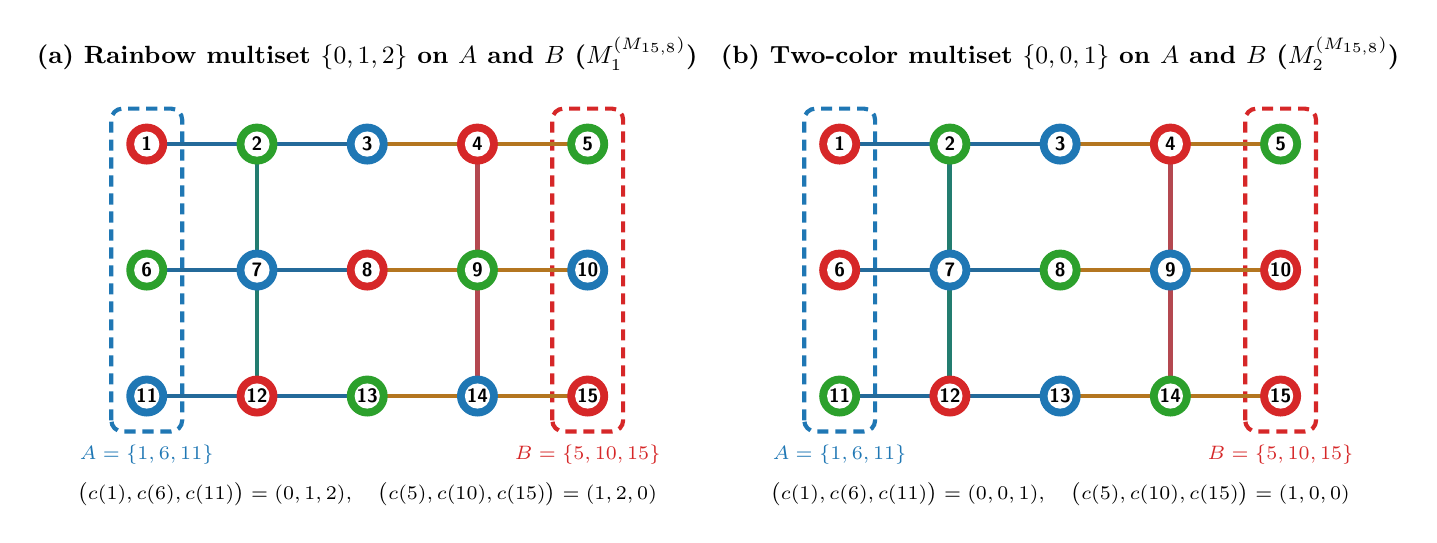
\begin{tikzpicture}[x=1cm,y=1cm]
  % --- Panel (a): Rainbow coloring M_1 ---
  \begin{scope}[shift={(-4.4,0)}]
    \node[font=\bfseries\small] at (0,3.15) {(a) Rainbow multiset $\{0,1,2\}$ on $A$ and $B$ ($M_1^{(M_{15,8})}$)};
    % Three horizontal 2-context chains: top (1..5), middle (6..10), bottom (11..15)
    \foreach \i/\x in {1/-2.8, 2/-1.4, 3/0.0, 4/1.4, 5/2.8} {
      \coordinate (a\i) at (\x, 2.0);
    }
    \foreach \i/\x in {6/-2.8, 7/-1.4, 8/0.0, 9/1.4, 10/2.8} {
      \coordinate (a\i) at (\x, 0.4);
    }
    \foreach \i/\x in {11/-2.8, 12/-1.4, 13/0.0, 14/1.4, 15/2.8} {
      \coordinate (a\i) at (\x,-1.2);
    }
    % Pseudocontext boxes
    \draw[CSmarkedA] (-3.25,-1.65) rectangle (-2.35,2.45);
    \node[font=\scriptsize\bfseries,text=colTwo] at (-2.8,-1.95) {$A=\{1,6,11\}$};
    \draw[CSmarkedB] ( 2.35,-1.65) rectangle ( 3.25,2.45);
    \node[font=\scriptsize\bfseries,text=colZero] at ( 2.8,-1.95) {$B=\{5,10,15\}$};
    % 8 contexts
    \draw[YOtrace,YOctx1]  (a1)--(a2)--(a3);
    \draw[YOtrace,YOctx9]  (a3)--(a4)--(a5);
    \draw[YOtrace,YOctx2]  (a6)--(a7)--(a8);
    \draw[YOtrace,YOctx13] (a8)--(a9)--(a10);
    \draw[YOtrace,YOctx3]  (a11)--(a12)--(a13);
    \draw[YOtrace,YOctx14] (a13)--(a14)--(a15);
    \draw[YOtrace,YOctx5]  (a2)--(a7)--(a12);
    \draw[YOtrace,YOctx10] (a4)--(a9)--(a14);
    % Vertices colored by c_1: 0=colZero(red), 1=colOne(green), 2=colTwo(blue)
    \foreach \v/\col in {1/colZero, 2/colOne, 3/colTwo, 4/colZero, 5/colOne,
                         6/colOne, 7/colTwo, 8/colZero, 9/colOne, 10/colTwo,
                         11/colTwo, 12/colZero, 13/colOne, 14/colTwo, 15/colZero} {
      \fill[\col] (a\v) circle[radius=0.26cm];
      \fill[white] (a\v) circle[radius=0.16cm];
      \node[YOnumber] at (a\v) {\v};
    }
    \node[font=\scriptsize] at (0,-2.45) {$\bigl(c(1),c(6),c(11)\bigr)=(0,1,2),\quad \bigl(c(5),c(10),c(15)\bigr)=(1,2,0)$};
  \end{scope}

  % --- Panel (b): Two-color multiset coloring M_2 ---
  \begin{scope}[shift={(4.4,0)}]
    \node[font=\bfseries\small] at (0,3.15) {(b) Two-color multiset $\{0,0,1\}$ on $A$ and $B$ ($M_2^{(M_{15,8})}$)};
    \foreach \i/\x in {1/-2.8, 2/-1.4, 3/0.0, 4/1.4, 5/2.8} {
      \coordinate (b\i) at (\x, 2.0);
    }
    \foreach \i/\x in {6/-2.8, 7/-1.4, 8/0.0, 9/1.4, 10/2.8} {
      \coordinate (b\i) at (\x, 0.4);
    }
    \foreach \i/\x in {11/-2.8, 12/-1.4, 13/0.0, 14/1.4, 15/2.8} {
      \coordinate (b\i) at (\x,-1.2);
    }
    \draw[CSmarkedA] (-3.25,-1.65) rectangle (-2.35,2.45);
    \node[font=\scriptsize\bfseries,text=colTwo] at (-2.8,-1.95) {$A=\{1,6,11\}$};
    \draw[CSmarkedB] ( 2.35,-1.65) rectangle ( 3.25,2.45);
    \node[font=\scriptsize\bfseries,text=colZero] at ( 2.8,-1.95) {$B=\{5,10,15\}$};
    \draw[YOtrace,YOctx1]  (b1)--(b2)--(b3);
    \draw[YOtrace,YOctx9]  (b3)--(b4)--(b5);
    \draw[YOtrace,YOctx2]  (b6)--(b7)--(b8);
    \draw[YOtrace,YOctx13] (b8)--(b9)--(b10);
    \draw[YOtrace,YOctx3]  (b11)--(b12)--(b13);
    \draw[YOtrace,YOctx14] (b13)--(b14)--(b15);
    \draw[YOtrace,YOctx5]  (b2)--(b7)--(b12);
    \draw[YOtrace,YOctx10] (b4)--(b9)--(b14);
    \foreach \v/\col in {1/colZero, 2/colOne, 3/colTwo, 4/colZero, 5/colOne,
                         6/colZero, 7/colTwo, 8/colOne, 9/colTwo, 10/colZero,
                         11/colOne, 12/colZero, 13/colTwo, 14/colOne, 15/colZero} {
      \fill[\col] (b\v) circle[radius=0.26cm];
      \fill[white] (b\v) circle[radius=0.16cm];
      \node[YOnumber] at (b\v) {\v};
    }
    \node[font=\scriptsize] at (0,-2.45) {$\bigl(c(1),c(6),c(11)\bigr)=(0,0,1),\quad \bigl(c(5),c(10),c(15)\bigr)=(1,0,0)$};
  \end{scope}
\end{tikzpicture}
\caption{Mayet's $15$-ray, $8$-context hypergraph $M_{15,8}$ in $\R^3$ [Eq.~\eqref{eq:M15-vectors}] with paired size-three affine pseudocontexts $A=\{1,6,11\}$ and $B=\{5,10,15\}$ (dashed boxes). Vertex outer rings indicate colors $0$ (red), $1$ (green), and $2$ (blue) for the two Context--Color Matrices in Eq.~\eqref{eq:M15-matrices}: (a) $M_1^{(M_{15,8})}$, where both $A$ and $B$ are rainbow $\{0,1,2\}$; (b) $M_2^{(M_{15,8})}$, where both $A$ and $B$ carry the two-color multiset $\{0,0,1\}$.}\label{fig:M15}
\end{figure*}

\subsection{Balanced Size-Three Pseudocontexts in \texorpdfstring{$B_{13,7}$}{B13,7} and \texorpdfstring{$R_{21,12},R_{25,15}$}{R21,12, R25,15}}\label{sec:B13-R21}

Two further families of faithfully coordinatized hypergraphs from Ref.~\cite{2026-latin-context-matrix} already contain balanced covering certificates for size-three affine pseudocontexts:
\begin{enumerate}
\item \emph{The $13$-ray, $7$-context Specker bug $B_{13,7}\subset\R^3$ ($N_c=6$, $|\Sc_{\mathrm{ext}}|/|\Sc|=12/14$):} Its $7$ contexts are $E_1=\{1,2,3\}$, $E_2=\{7,8,9\}$, $E_3=\{2,8,5\}$, $E_4=\{3,11,14\}$, $E_5=\{7,11,15\}$, $E_6=\{9,10,23\}$, and $E_7=\{1,10,19\}$ [Fig.~\ref{fig:3d-gadgets}(a)], with Yu--Oh coordinates from Table~\ref{tab:yo-vectors}. The six outer contexts partition into two $3$-context coverings $\mathcal{F}_+=\{E_1,E_5,E_6\}$ and $\mathcal{F}_-=\{E_2,E_4,E_7\}$ of $(V\setminus\{5\})\setminus B$ and $(V\setminus\{5\})\setminus A$, where
\begin{equation}\label{eq:B13-paired3}
A=\{2,15,23\},\qquad B=\{8,14,19\}.
\end{equation}
Hence $(\chi_{E_1}+\chi_{E_5}+\chi_{E_6})-(\chi_{E_2}+\chi_{E_4}+\chi_{E_7})=\chi_A-\chi_B$, forcing $\{\!\{c(2),c(15),c(23)\}\!\}=\{\!\{c(8),c(14),c(19)\}\!\}$ across all $N_c=6$ normalized $7\times 3$ Context--Color Matrices (and likewise in the $4$-dimensional common-apex lift $B_{14,7}^{(4)}$).

\item \emph{Gaussian-integer row--column hub grids $R_{21,12}$ and $R_{25,15}$ in $\C^3$~\cite[Sec.~IV\,D]{2026-latin-context-matrix}:} In $R_{21,12}$ ($N_c=32$, $|\Sc_{\mathrm{ext}}|/|\Sc|=48/54$) and $R_{25,15}$ ($N_c=24$, $|\Sc_{\mathrm{ext}}|/|\Sc|=48/81$), the $3\times 3$ core grid has row contexts $R_1=\{1,2,3\}$, $R_2=\{4,5,6\}$, $R_3=\{7,8,9\}$ and hub contexts $\{1,10,13\}$, $\{2,11,14\}$, $\{3,12,15\}$ (for $R_1$), $\{4,10,16\}$, $\{5,11,17\}$, $\{6,12,18\}$ (for $R_2$), and $\{7,10,19\}$, $\{8,11,20\}$, $\{9,12,21\}$ (for $R_3$). For any two rows (say $R_1$ and $R_2$) and any column $j\in\{1,2,3\}$ (say $j=1$), the two $3$-context families $\mathcal{F}_+=\{\{1,2,3\},\{4,10,16\},\{2,11,14\},\{3,12,15\}\}\setminus\{\{1,2,3\}\}$ combine to yield $12$ size-three affine pseudocontexts such as
\begin{equation}\label{eq:R21-paired3}
A=\{1,17,18\},\qquad B=\{4,14,15\},
\end{equation}
via the balanced $3$-context identity $(\chi_{\{1,2,3\}}+\chi_{\{5,11,17\}}+\chi_{\{6,12,18\}})-(\chi_{\{4,5,6\}}+\chi_{\{2,11,14\}}+\chi_{\{3,12,15\}})=\chi_{\{1,17,18\}}-\chi_{\{4,14,15\}}$, forcing $\{\!\{c(1),c(17),c(18)\}\!\}=\{\!\{c(4),c(14),c(15)\}\!\}$ in all $32$ (resp.\ $24$) normalized Context--Color Matrices.
\end{enumerate}

\subsection{The \texorpdfstring{$20$}{20}-Ray, \texorpdfstring{$12$}{12}-Context Complex Octagon \texorpdfstring{$\Htwenty\subset\C^3$}{H20 in C3}}\label{sec:octagon}

To reach target size $k=2$ via a balanced covering certificate, one must pass from $\R^3$ to $\C^3$~\cite{2026-Navara-Svozil-pseudocontexts,2026-Navara-Svozil-complex-only-3d-hypergraphs}. The $20$-ray, $12$-context octagon $\Htwenty$ (Fig.~\ref{fig:octagon}) has eight perimeter contexts $E_j=\{v_{j-1,j},v_j,v_{j,j+1}\}$ ($j\in\Z_8$) and four inner contexts $D_0=\{v_0,a_1,v_4\}$, $D_2=\{v_2,a_2,v_6\}$, $D_1=\{v_1,b_2,v_5\}$, $D_3=\{v_3,b_1,v_7\}$. The two $6$-context coverings $\mathcal{G}_+=\{D_0,D_2,E_1,E_3,E_5,E_7\}$ and $\mathcal{G}_-=\{D_1,D_3,E_0,E_2,E_4,E_6\}$ yield $\sum_{C\in\mathcal{G}_+}\chi_C-\sum_{C\in\mathcal{G}_-}\chi_C=\chi_A-\chi_B$ for the nonorthogonal pairs
\begin{equation}\label{eq:octagon-targets}
A=\{a_1,a_2\},\qquad B=\{b_1,b_2\}.
\end{equation}

Exhaustive computation gives $|\Sc(\Htwenty)|=|\Sc_{\mathrm{ext}}(\Htwenty)|=26$ two-valued states and $N_c=12$ normalized $12\times 3$ Context--Color Matrices (with anchor $E_0=(v_{70},v_0,v_{01})$). Across all $12$ normalized colorings, $\{\!\{c(a_1),c(a_2)\}\!\}=\{\!\{c(b_1),c(b_2)\}\!\}$ holds identically: $4$ colorings assign monochromatic multisets ($2$ with $\{0,0\}$ and $2$ with $\{2,2\}$) and $8$ assign bichromatic multisets ($2$ with $\{0,1\}$, $4$ with $\{0,2\}$, and $2$ with $\{1,2\}$). Representative bichromatic ($M_1^{(\Htwenty)}$) and monochromatic ($M_2^{(\Htwenty)}$) Context--Color Matrices are:
\begin{equation}\label{eq:octagon-matrices}
\setlength{\arraycolsep}{2.2pt}
M_1^{(\Htwenty)}=\begin{pmatrix}
\mathbf{c}_0&\mathbf{c}_1&\mathbf{c}_2\\\hline
v_{70}&v_0&v_{01}\\
v_1&v_{12}&v_{01}\\
v_{23}&v_{12}&v_2\\
v_{23}&v_{34}&v_3\\
v_4&v_{34}&v_{45}\\
v_{56}&v_5&v_{45}\\
v_{56}&v_6&v_{67}\\
v_{70}&v_7&v_{67}\\\hline
v_4&v_0&\mathbf{a_1}\\
\mathbf{a_2}&v_6&v_2\\
v_1&v_5&\mathbf{b_2}\\
\mathbf{b_1}&v_7&v_3
\end{pmatrix},\quad
M_2^{(\Htwenty)}=\begin{pmatrix}
\mathbf{c}_0&\mathbf{c}_1&\mathbf{c}_2\\\hline
v_{70}&v_0&v_{01}\\
v_{12}&v_1&v_{01}\\
v_{12}&v_2&v_{23}\\
v_{34}&v_3&v_{23}\\
v_{34}&v_{45}&v_4\\
v_{56}&v_{45}&v_5\\
v_{56}&v_{67}&v_6\\
v_{70}&v_{67}&v_7\\\hline
\mathbf{a_1}&v_0&v_4\\
\mathbf{a_2}&v_2&v_6\\
\mathbf{b_2}&v_1&v_5\\
\mathbf{b_1}&v_3&v_7
\end{pmatrix}.
\end{equation}

\begin{figure}[!htbp]
\centering
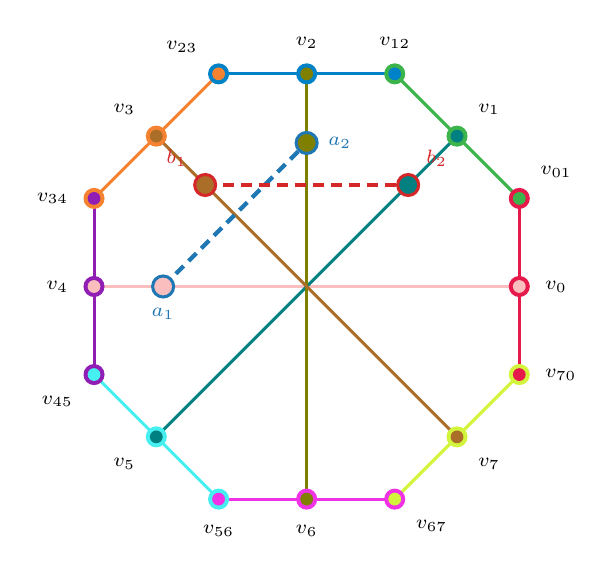
\begin{tikzpicture}[scale=1.35,every label/.style={font=\scriptsize}]
  \def\Rmid{2.0}
  \def\Rcor{2.1648}
  \def\Rinn{1.35}
  \foreach \i/\j/\ang in {
    0/1/22.5,1/2/67.5,2/3/112.5,3/4/157.5,
    4/5/202.5,5/6/247.5,6/7/292.5,7/0/337.5
  }{\coordinate (v\i\j) at (\ang:\Rcor);}
  \foreach \i/\ang in {
    0/0,1/45,2/90,3/135,4/180,5/225,6/270,7/315
  }{\coordinate (v\i) at (\ang:\Rmid);}
  \coordinate (a1) at (180:\Rinn);
  \coordinate (a2) at (90:\Rinn);
  \coordinate (b1) at (135:\Rinn);
  \coordinate (b2) at (45:\Rinn);

  \draw[ctxline,draw=ctx1] (v70)--(v01);
  \draw[ctxline,draw=ctx2] (v01)--(v12);
  \draw[ctxline,draw=ctx3] (v12)--(v23);
  \draw[ctxline,draw=ctx4] (v23)--(v34);
  \draw[ctxline,draw=ctx5] (v34)--(v45);
  \draw[ctxline,draw=ctx6] (v45)--(v56);
  \draw[ctxline,draw=ctx7] (v56)--(v67);
  \draw[ctxline,draw=ctx8] (v67)--(v70);
  \draw[ctxline,draw=ctx9] (v0)--(v4);
  \draw[ctxline,draw=ctx10] (v1)--(v5);
  \draw[ctxline,draw=ctx11] (v2)--(v6);
  \draw[ctxline,draw=ctx12] (v3)--(v7);

  % Highlight size-2 pseudocontexts A={a1,a2} and B={b1,b2}
  \draw[CSmarkedA] (a1) -- (a2);
  \draw[CSmarkedB] (b1) -- (b2);

  \twodotlabel{ctx1}{ctx2}{above right}{$v_{01}$}{(v01)}
  \twodotlabel{ctx2}{ctx3}{above}{$v_{12}$}{(v12)}
  \twodotlabel{ctx3}{ctx4}{above left}{$v_{23}$}{(v23)}
  \twodotlabel{ctx4}{ctx5}{left}{$v_{34}$}{(v34)}
  \twodotlabel{ctx5}{ctx6}{below left}{$v_{45}$}{(v45)}
  \twodotlabel{ctx6}{ctx7}{below}{$v_{56}$}{(v56)}
  \twodotlabel{ctx7}{ctx8}{below right}{$v_{67}$}{(v67)}
  \twodotlabel{ctx8}{ctx1}{right}{$v_{70}$}{(v70)}
  \twodotlabel{ctx1}{ctx9}{right}{$v_0$}{(v0)}
  \twodotlabel{ctx2}{ctx10}{above right}{$v_1$}{(v1)}
  \twodotlabel{ctx3}{ctx11}{above}{$v_2$}{(v2)}
  \twodotlabel{ctx4}{ctx12}{above left}{$v_3$}{(v3)}
  \twodotlabel{ctx5}{ctx9}{left}{$v_4$}{(v4)}
  \twodotlabel{ctx6}{ctx10}{below left}{$v_5$}{(v5)}
  \twodotlabel{ctx7}{ctx11}{below}{$v_6$}{(v6)}
  \twodotlabel{ctx8}{ctx12}{below right}{$v_7$}{(v7)}
  \node[circle,fill=ctx9,draw=colTwo,line width=1.1pt,minimum size=7.6pt,inner sep=0pt,
        label={[font=\scriptsize\bfseries,text=colTwo]below:{$a_1$}}] at (a1) {};
  \node[circle,fill=ctx11,draw=colTwo,line width=1.1pt,minimum size=7.6pt,inner sep=0pt,
        label={[font=\scriptsize\bfseries,text=colTwo]right:{$a_2$}}] at (a2) {};
  \node[circle,fill=ctx12,draw=colZero,line width=1.1pt,minimum size=7.6pt,inner sep=0pt,
        label={[font=\scriptsize\bfseries,text=colZero]above left:{$b_1$}}] at (b1) {};
  \node[circle,fill=ctx10,draw=colZero,line width=1.1pt,minimum size=7.6pt,inner sep=0pt,
        label={[font=\scriptsize\bfseries,text=colZero]above right:{$b_2$}}] at (b2) {};
\end{tikzpicture}
\caption{The $20$-ray, $12$-context complex octagon $\Htwenty\subset\C^3$~\cite{2026-Navara-Svozil-pseudocontexts,2026-Navara-Svozil-complex-only-3d-hypergraphs}. The two nonorthogonal target pairs $A=\{a_1,a_2\}$ (blue dashed link) and $B=\{b_1,b_2\}$ (red dashed link) carry identical $2$-element color multisets $\{\!\{c(a_1),c(a_2)\}\!\}=\{\!\{c(b_1),c(b_2)\}\!\}$ across all $N_c=12$ normalized $12\times 3$ Context--Color Matrices [Eq.~\eqref{eq:octagon-matrices}].}\label{fig:octagon}
\end{figure}

% ==================================================================
\subsection{Color-Weighted Eigensystems of the Affine Pairs}\label{sec:weighted-affine}

The affine certificate gives $O_A(\mathbf1)=O_B(\mathbf1)$ in every FOR. For general color values, construct the signed operator
\begin{equation}\label{eq:weighted-pair-difference}
\begin{aligned}
D_{A,B}(\mathbf c;\kappa)&=O_A(\mathbf c;\kappa)-O_B(\mathbf c;\kappa),\\
\max_\rho\Tr(\rho D_{A,B})&=\lambda_{\max}(D_{A,B}).
\end{aligned}
\end{equation}
Color-multiset conservation implies $\Tr D_{A,B}=0$, whereas the affine certificate implies invariance under $\mathbf c\mapsto\mathbf c+\tau\mathbf1$. It does not generally imply $D_{A,B}=0$ for unequal color values. The maximum is positive whenever $D_{A,B}\ne0$, because a nonzero traceless Hermitian operator has both positive and negative eigenvalues. In dimension three its characteristic equality is
\begin{equation}\label{eq:weighted-pair-cubic}
\lambda^3-\tfrac12\Tr(D_{A,B}^2)\lambda-\det D_{A,B}=0.
\end{equation}
Its maximum is $F(0,-\Tr(D_{A,B}^2)/2,\det D_{A,B})$, with eigenspaces given by Eq.~\eqref{eq:weighted-spectral-resolution}.

For Mayet's rainbow coloring $M_1^{(M_{15,8})}$, the ordered triples $A=(1,6,11)$ and $B=(5,10,15)$ carry weights $(c_0,c_1,c_2)$ and $(c_1,c_2,c_0)$, respectively. Directly forming the projectors from Eq.~\eqref{eq:M15-vectors} gives
\begin{equation}\label{eq:weighted-M15}
\begin{aligned}
t&=c_0+c_1+c_2,\qquad \delta=\tfrac27c_0c_1c_2,\\
b_A&=\tfrac34c_0c_1+\tfrac{27}{28}c_0c_2+\tfrac37c_1c_2,\\
b_B&=\tfrac34c_1c_2+\tfrac{27}{28}c_0c_1+\tfrac37c_0c_2,\\
\max_\rho\Tr(\rho O_A)&=F(t,b_A,\delta),\\
\max_\rho\Tr(\rho O_B)&=F(t,b_B,\delta).
\end{aligned}
\end{equation}
For their difference, the two coefficients in Eq.~\eqref{eq:weighted-pair-cubic} are explicitly
\begin{equation}\label{eq:weighted-M15-difference}
\begin{aligned}
\tfrac12\Tr D_{A,B}^2={}&\tfrac3{700}\bigl(57c_0^2+119c_1^2+72c_2^2\\
&\hspace{1.2em}-104c_0c_1-10c_0c_2-134c_1c_2\bigr),\\
\det D_{A,B}={}&\tfrac{27}{350}(c_0-c_1)(c_0-c_2)(c_1-c_2).
\end{aligned}
\end{equation}
At $c_0=c_1=c_2=1$, the common operator has eigenvalues $2$ and $\tfrac12\pm\tfrac{\sqrt{21}}{14}$, so its maximal expectation is exactly $2$. The two-color coloring $M_2^{(M_{15,8})}$ is covered by the same projector construction, with weights $(c_0,c_0,c_1)$ on $A$ and $(c_1,c_0,c_0)$ on $B$.

The other displayed size-three affine pairs have equally short characteristic equalities. Table~\ref{tab:weighted-affine-triples} gives the four coordinate-dependent coefficients of Eq.~\eqref{eq:weighted-triple-coefficients}. The weights $a_i$ are the color values on the ordered vertices, so repeated colors are included. In every row,
\begin{equation}\label{eq:weighted-affine-triple-max}
\max_\rho\Tr(\rho O_X)
=F\left(\sum_i a_i,\sum_{i<j}h_{ij}a_ia_j,g\prod_i a_i\right).
\end{equation}
The Gaussian-integer coordinates for the hub-grid row are those printed in Ref.~\cite[Sec.~IV\,D]{2026-latin-context-matrix}; the same target rays occur in $R_{21,12}$ and $R_{25,15}$. The principal-minor formula also treats the remaining affine pairs without an additional assumption about their color patterns.

\begin{table}[t]
\caption{Exact Gram coefficients for the ordered affine target triples. Both listed sides have the coefficients shown, in their respective displayed order. Color weights must be assigned according to the chosen coloring.}\label{tab:weighted-affine-triples}
\footnotesize\setlength{\tabcolsep}{3pt}
\begin{ruledtabular}
\begin{tabular}{lcccc}
Ordered targets & $h_{01}$ & $h_{02}$ & $h_{12}$ & $g$\\\hline
$M_{15,8}$: $(1,6,11)$, $(5,10,15)$ & $3/4$ & $27/28$ & $3/7$ & $2/7$\\
$B_{13,7}$: $(2,15,23)$, $(8,14,19)$ & $5/6$ & $5/6$ & $5/9$ & $4/9$\\
$R_{21,12},R_{25,15}$: & & & &\\[-2pt]
\quad $(1,17,18)$, $(4,14,15)$ & $9/10$ & $9/10$ & $3/4$ & $13/20$
\end{tabular}
\end{ruledtabular}
\end{table}

For the complex octagon, choose the target coordinates of the FOR in Ref.~\cite{2026-Navara-Svozil-complex-only-3d-hypergraphs},
\begin{equation}\label{eq:weighted-octagon-rays}
\begin{aligned}
q_{a_1}&=(s,1,0),&q_{a_2}&=(s,-1,0),\\
q_{b_1}&=(s,\eta,0),&q_{b_2}&=(s,-\eta,0),\\
s^2&=\frac{49-5\sqrt{69}}{26},&\eta&=\frac{5+12i}{13}.
\end{aligned}
\end{equation}
Here $|\ip{\hat q_{a_1}}{\hat q_{a_2}}|^2=|\ip{\hat q_{b_1}}{\hat q_{b_2}}|^2=23/75$. In the bichromatic coloring $M_1^{(\Htwenty)}$, $A$ has weights $(c_2,c_0)$ and $B$ has weights $(c_0,c_2)$. Both weighted operators have eigenvalues
\begin{equation}\label{eq:weighted-octagon-spectrum}
0,\qquad \lambda_\pm=\frac{c_0+c_2\pm
\sqrt{(c_0-c_2)^2+\tfrac{92}{75}c_0c_2}}{2}.
\end{equation}
Their individual maximal expectations equal $\max\{0,\lambda_+\}$. They are isospectral even though their difference need not vanish. Indeed,
\begin{equation}\label{eq:weighted-octagon-difference}
\begin{aligned}
D_{A,B}&=(c_2-c_0)(P_{a_1}-P_{b_2}),\\
\operatorname{spec}D_{A,B}&=\left\{0,\ \pm\tfrac{2\sqrt3}{5}(c_2-c_0)\right\},\\
\max_\rho\Tr(\rho D_{A,B})&=\tfrac{2\sqrt3}{5}|c_2-c_0|.
\end{aligned}
\end{equation}
For an explicit eigensystem, put $z=s(1+\bar\eta)/(1+s^2)$, so $|z|=2\sqrt3/5$. The unit vectors $2^{-1/2}(z/|z|,\pm1,0)^{\mathsf T}$ have eigenvalues $\pm(c_2-c_0)|z|$, while $(0,0,1)^{\mathsf T}$ has eigenvalue zero. If $c_2=c_0$, the whole space is the zero eigenspace. In the monochromatic coloring $M_2^{(\Htwenty)}$, $D_{A,B}=0$ for all color values, and the two individual spectra are $\{0,c_0(1\pm\sqrt{23/75})\}$.

\subsection{Classical Bounds for the Affine Pairs}\label{sec:classical-affine}

For Mayet's ordered target $A=(1,6,11)$ in its rainbow coloring, all $24$ two-valued states restrict to the seven binary patterns other than $(1,1,1)$. The exact classical envelope is therefore the minimum and maximum of
\begin{equation}\label{eq:classical-M15-single}
\{0,c_0,c_1,c_2,c_0+c_1,c_0+c_2,c_1+c_2\}.
\end{equation}
At unit values the classical interval is $[0,2]$, containing the quantum interval $[\tfrac12-\sqrt{21}/14,2]$. For the signed pair in the displayed rainbow coloring, the distinct coefficient vectors are zero and $e_i-e_j$ ($i\ne j$). Consequently,
\begin{equation}\label{eq:classical-M15-pair}
\begin{aligned}
\beta^+_{\Sc}(\mathbf c)&=\max_jc_j-\min_jc_j,\\
\beta^-_{\Sc}(\mathbf c)&=-\beta^+_{\Sc}(\mathbf c).
\end{aligned}
\end{equation}
This is the classical comparison for the spectrum in Eq.~\eqref{eq:weighted-M15-difference}; positivity of its largest eigenvalue alone is not a violation of Eq.~\eqref{eq:classical-M15-pair}.

For the complex octagon's size-two target, all four binary restrictions occur, so the individual weighted bounds are
\begin{equation}\label{eq:classical-octagon-envelope}
\beta^-_{\Sc}=\sum_{j\in\kappa(A)}\min(0,c_j),\qquad
\beta^+_{\Sc}=\sum_{j\in\kappa(A)}\max(0,c_j)
\end{equation}
in a bichromatic coloring. Its unit-weight quantum interval $[0,1+\sqrt{23/75}]$ is contained in the classical interval $[0,2]$. The primary triples of $R_{21,12}$ and $R_{25,15}$ realize all eight binary patterns; their individual rainbow-weight bounds are similarly the sums of the negative and positive parts of the three color values. The full facet/equality comparison finds no separating color weights among the tested single or paired expressions for these two FORs, Mayet's FOR, or the complex octagon FOR. The exact envelopes of every color pattern and every pair are retained in the computational tables.

The enumeration also corrects the octagon census: besides its single size-two pair, it has $20$ non-twin size-three pairs satisfying Definition~\ref{def:chromatic-relations}. All $20$ admit balanced affine certificates. For example,
\begin{equation}\label{eq:octagon-size3-correction}
\begin{aligned}
A_3&=\{a_1,v_{12},v_{56}\},\\
B_3&=\{b_2,v_{34},v_{70}\},\\
\chi_{A_3}-\chi_{B_3}
&=\chi_{D_0}+\chi_{E_1}+\chi_{E_5}\\
&\quad-\chi_{D_1}-\chi_{E_0}-\chi_{E_4}.
\end{aligned}
\end{equation}
Both triples are independent and disjoint in the same FOR. The original manuscript verifier independently reproduces the count $20$, now recorded in Table~\ref{tab:master-chromatic-relations}.

% ==================================================================
\section{A Two-Valued State Admissibility Context in \texorpdfstring{$\R^3$}{R3}}\label{sec:two-valued}
% ==================================================================

We first realize the stronger alternative in Definition~\ref{def:admissibility-context}: an independent triple normalized on \emph{every} two-valued state. The construction pastes two standard nonseparating gadgets at one ray. Its logical proof is independent of the subsequent enumeration, and an explicit FOR makes the distinction from affine and operator normalization concrete.

\subsection{A Completed Nonseparating Gadget}

Write $\mathcal B(a,b;x)$ for the seven-context Specker bug
\begin{equation}\label{eq:H53-bug}
\begin{gathered}
\{a,x_1,x_2\},\quad\{x_2,x_3,x_4\},\\
\{x_4,x_5,b\},\quad\{b,x_6,x_7\},\\
\{x_7,x_8,x_9\},\quad\{x_9,x_{10},a\},\\
\{x_3,x_8,x_{11}\}.
\end{gathered}
\end{equation}
Every two-valued state satisfies $s(a)+s(b)\le1$. Indeed, assigning one to both endpoints forces $s(x_2)=s(x_4)=s(x_7)=s(x_9)=0$, hence $s(x_3)=s(x_8)=1$, contradicting the final context.

Let $G$ be the $27$-ray, $17$-context gadget formed by
\begin{equation}\label{eq:H53-G}
\begin{gathered}
\mathcal B(a,b;x),\quad\mathcal B(b',a';y),\\
\{a,c,b'\},\quad\{b,c,a'\},\quad\{c,x_{11},y_{11}\}.
\end{gathered}
\end{equation}
This is a completed realization of the Kochen--Specker $\Gamma_3$ nonseparating construction~\cite{kochen1,svozil-2018-whycontexts}. The last context completes an orthogonal triple in the FOR below; the logical identity already follows from the other $16$ contexts. In Fig.~\ref{fig:H53-34}, the labels $E_{15},E_{16},E_{17}$ follow the order of these three additional contexts; $E_{32},E_{33},E_{34}$ label the corresponding contexts of the second copy. Each repeated label pairs the two branches of one context through its intertwining vertex.

\begin{lemma}[Two-Valued Nonseparation]\label{lem:H53-nonseparation}
Every $s\in\Sc(G)$ satisfies
\begin{equation}\label{eq:H53-nonseparation}
\begin{gathered}
s(a)=s(a'),\qquad s(b)=s(b'),\\
s(a)+s(b)+s(c)=1.
\end{gathered}
\end{equation}
\end{lemma}
\begin{proof}
If $s(a)=1$, the first bug forces $s(b)=0$, and $\{a,c,b'\}$ forces $s(c)=s(b')=0$. The context $\{b,c,a'\}$ then gives $s(a')=1$. Conversely, if $s(a')=1$, the second bug forces $s(b')=0$, while $\{b,c,a'\}$ forces $s(b)=s(c)=0$; now $\{a,c,b'\}$ gives $s(a)=1$. Thus $s(a)=s(a')$. The symmetric argument gives $s(b)=s(b')$. Substitution into $s(a)+s(c)+s(b')=1$ proves the final identity.
\end{proof}

\subsection{One-Vertex Pasting and Universal Admissibility}

Take a second copy $\widetilde G$ and identify only its $\widetilde a$ with the first copy's $c$. Write $u=\widetilde{a'}$. The union $H_{53,34}=G\cup\widetilde G$ has $27+27-1=53$ rays and $17+17=34$ contexts, all drawn in Fig.~\ref{fig:H53-34}.

\begin{theorem}[Two-Valued State Admissibility on Nonadjacent Rays]\label{thm:H53-two-valued}
The hypergraph $H_{53,34}$ admits a FOR in $\R^3$ in which $U=\{a,b,u\}$ is pairwise nonorthogonal. Its two-valued state space is nonempty and
\begin{equation}\label{eq:H53-exactone}
s(a)+s(b)+s(u)=1\qquad\forall s\in\Sc(H_{53,34}).
\end{equation}
Thus $U$ is a two-valued state admissibility context and, in particular, a chromatic admissible context.
\end{theorem}
\begin{proof}
Restrict any two-valued state to each copy of $G$. Lemma~\ref{lem:H53-nonseparation} gives $s(a)+s(b)+s(c)=1$ in the first copy and $s(c)=s(u)$ in the second, proving Eq.~\eqref{eq:H53-exactone}. The representation below verifies pairwise nonorthogonality and faithfulness. The enumeration in Eq.~\eqref{eq:H53-patterns} establishes nonemptiness and shows that each distinguished vertex can be true. Every color-class state of every strong $3$-coloring is a two-valued state, so Theorem~\ref{thm:chromatic-conservation}(1) gives universal chromatic completeness as well.
\end{proof}

\begin{figure*}[!t]
\centering
% H_{53,34}: all 53 rays and all 34 contexts; color supplements labels and shapes.
% E15/E16/E17 and E33/E34 share horizontal tangents, as required by smooth vertical symmetry.
\definecolor{h53red}{HTML}{B44850}
\definecolor{h53blue}{HTML}{246A9A}
\definecolor{h53green}{HTML}{237D70}
\definecolor{h53gold}{HTML}{B47620}
\definecolor{h53purple}{HTML}{85458B}
\definecolor{h53cyan}{HTML}{408B9C}
\definecolor{h53brown}{HTML}{966E4C}
\definecolor{h53target}{HTML}{C66F12}
\begin{tikzpicture}[x=1.06cm,y=1.06cm,
  context/.style={draw=black,line width=1.0pt,line cap=butt,line join=miter,preaction={draw=white,line width=3.0pt}},
  ray/.style={circle,draw=black,fill=white,inner sep=0pt,minimum size=3.7pt,line width=.5pt},
  target/.style={circle,draw=h53target,double,double distance=1pt,fill=none,inner sep=0pt,minimum size=11.4pt,line width=.65pt},
  shared/.style={rectangle,draw=h53blue,fill=none,inner sep=0pt,minimum size=14.0pt,line width=1pt},
  raylabel/.style={font=\fontsize{8}{8}\selectfont,inner sep=.6pt,fill=white},
  bugtitle/.style={font=\small,inner sep=2pt,fill=white},
  edgekey/.style={font=\fontsize{8}{8}\selectfont,fill=white,inner sep=1.2pt},
  bugframe/.style={draw=black!50,densely dotted,line width=.45pt,rounded corners=3pt}]
  \draw[bugframe] (-6.02,2.04) rectangle (-1.56,5.80);
  \draw[bugframe] (1.56,2.04) rectangle (6.02,5.80);
  \draw[bugframe] (-2.22,-3.66) rectangle (1.68,.36);
  \draw[bugframe] (3.32,-3.66) rectangle (7.23,.36);
  \coordinate (v-a) at (-5.40000,3.60000); % ray: a
  \coordinate (v-b) at (-2.20000,3.60000); % ray: b
  \coordinate (v-x1) at (-5.00000,4.15000); % ray: x1
  \coordinate (v-x2) at (-4.60000,4.70000); % ray: x2
  \coordinate (v-x3) at (-3.80000,4.70000); % ray: x3
  \coordinate (v-x4) at (-3.00000,4.70000); % ray: x4
  \coordinate (v-x5) at (-2.60000,4.15000); % ray: x5
  \coordinate (v-x6) at (-2.60000,3.05000); % ray: x6
  \coordinate (v-x7) at (-3.00000,2.50000); % ray: x7
  \coordinate (v-x8) at (-3.80000,2.50000); % ray: x8
  \coordinate (v-x9) at (-4.60000,2.50000); % ray: x9
  \coordinate (v-x10) at (-5.00000,3.05000); % ray: x10
  \coordinate (v-x11) at (-3.80000,3.60000); % ray: x11
  \coordinate (v-bp) at (5.40000,3.60000); % ray: bp
  \coordinate (v-ap) at (2.20000,3.60000); % ray: ap
  \coordinate (v-y1) at (5.00000,4.15000); % ray: y1
  \coordinate (v-y2) at (4.60000,4.70000); % ray: y2
  \coordinate (v-y3) at (3.80000,4.70000); % ray: y3
  \coordinate (v-y4) at (3.00000,4.70000); % ray: y4
  \coordinate (v-y5) at (2.60000,4.15000); % ray: y5
  \coordinate (v-y6) at (2.60000,3.05000); % ray: y6
  \coordinate (v-y7) at (3.00000,2.50000); % ray: y7
  \coordinate (v-y8) at (3.80000,2.50000); % ray: y8
  \coordinate (v-y9) at (4.60000,2.50000); % ray: y9
  \coordinate (v-y10) at (5.00000,3.05000); % ray: y10
  \coordinate (v-y11) at (3.80000,3.60000); % ray: y11
  \coordinate (v-c) at (-0.00000,0.00000); % ray: c
  \coordinate (v-t-b) at (0.00000,-3.20000); % ray: t_b
  \coordinate (v-t-x1) at (0.55000,-0.40000); % ray: t_x1
  \coordinate (v-t-x2) at (1.10000,-0.80000); % ray: t_x2
  \coordinate (v-t-x3) at (1.10000,-1.60000); % ray: t_x3
  \coordinate (v-t-x4) at (1.10000,-2.40000); % ray: t_x4
  \coordinate (v-t-x5) at (0.55000,-2.80000); % ray: t_x5
  \coordinate (v-t-x6) at (-0.55000,-2.80000); % ray: t_x6
  \coordinate (v-t-x7) at (-1.10000,-2.40000); % ray: t_x7
  \coordinate (v-t-x8) at (-1.10000,-1.60000); % ray: t_x8
  \coordinate (v-t-x9) at (-1.10000,-0.80000); % ray: t_x9
  \coordinate (v-t-x10) at (-0.55000,-0.40000); % ray: t_x10
  \coordinate (v-t-x11) at (0.00000,-1.60000); % ray: t_x11
  \coordinate (v-t-bp) at (5.00000,0.00000); % ray: t_bp
  \coordinate (v-u) at (5.00000,-3.20000); % ray: u
  \coordinate (v-t-y1) at (5.55000,-0.40000); % ray: t_y1
  \coordinate (v-t-y2) at (6.10000,-0.80000); % ray: t_y2
  \coordinate (v-t-y3) at (6.10000,-1.60000); % ray: t_y3
  \coordinate (v-t-y4) at (6.10000,-2.40000); % ray: t_y4
  \coordinate (v-t-y5) at (5.55000,-2.80000); % ray: t_y5
  \coordinate (v-t-y6) at (4.45000,-2.80000); % ray: t_y6
  \coordinate (v-t-y7) at (3.90000,-2.40000); % ray: t_y7
  \coordinate (v-t-y8) at (3.90000,-1.60000); % ray: t_y8
  \coordinate (v-t-y9) at (3.90000,-0.80000); % ray: t_y9
  \coordinate (v-t-y10) at (4.45000,-0.40000); % ray: t_y10
  \coordinate (v-t-y11) at (5.00000,-1.60000); % ray: t_y11
  \coordinate (v-t-c) at (2.50000,-6.30000); % ray: t_c
  % context 01: a,x1,x2
  \draw[context,draw=h53red] (v-a)--(v-x1)--(v-x2);
  % context 02: x2,x3,x4
  \draw[context,draw=h53blue] (v-x2)--(v-x3)--(v-x4);
  % context 03: x4,x5,b
  \draw[context,draw=h53green] (v-x4)--(v-x5)--(v-b);
  % context 04: b,x6,x7
  \draw[context,draw=h53gold] (v-b)--(v-x6)--(v-x7);
  % context 05: x7,x8,x9
  \draw[context,draw=h53purple] (v-x7)--(v-x8)--(v-x9);
  % context 06: x9,x10,a
  \draw[context,draw=h53cyan] (v-x9)--(v-x10)--(v-a);
  % context 07: x3,x11,x8
  \draw[context,draw=h53brown] (v-x3)--(v-x11)--(v-x8);
  % context 08: bp,y1,y2
  \draw[context,draw=h53red] (v-bp)--(v-y1)--(v-y2);
  % context 09: y2,y3,y4
  \draw[context,draw=h53blue] (v-y2)--(v-y3)--(v-y4);
  % context 10: y4,y5,ap
  \draw[context,draw=h53green] (v-y4)--(v-y5)--(v-ap);
  % context 11: ap,y6,y7
  \draw[context,draw=h53gold] (v-ap)--(v-y6)--(v-y7);
  % context 12: y7,y8,y9
  \draw[context,draw=h53purple] (v-y7)--(v-y8)--(v-y9);
  % context 13: y9,y10,bp
  \draw[context,draw=h53cyan] (v-y9)--(v-y10)--(v-bp);
  % context 14: y3,y11,y8
  \draw[context,draw=h53brown] (v-y3)--(v-y11)--(v-y8);
  % context 18: c,t_x1,t_x2
  \draw[context,draw=h53red] (v-c)--(v-t-x1)--(v-t-x2);
  % context 19: t_x2,t_x3,t_x4
  \draw[context,draw=h53blue] (v-t-x2)--(v-t-x3)--(v-t-x4);
  % context 20: t_x4,t_x5,t_b
  \draw[context,draw=h53green] (v-t-x4)--(v-t-x5)--(v-t-b);
  % context 21: t_b,t_x6,t_x7
  \draw[context,draw=h53gold] (v-t-b)--(v-t-x6)--(v-t-x7);
  % context 22: t_x7,t_x8,t_x9
  \draw[context,draw=h53purple] (v-t-x7)--(v-t-x8)--(v-t-x9);
  % context 23: t_x9,t_x10,c
  \draw[context,draw=h53cyan] (v-t-x9)--(v-t-x10)--(v-c);
  % context 24: t_x3,t_x11,t_x8
  \draw[context,draw=h53brown] (v-t-x3)--(v-t-x11)--(v-t-x8);
  % context 25: t_bp,t_y1,t_y2
  \draw[context,draw=h53red] (v-t-bp)--(v-t-y1)--(v-t-y2);
  % context 26: t_y2,t_y3,t_y4
  \draw[context,draw=h53blue] (v-t-y2)--(v-t-y3)--(v-t-y4);
  % context 27: t_y4,t_y5,u
  \draw[context,draw=h53green] (v-t-y4)--(v-t-y5)--(v-u);
  % context 28: u,t_y6,t_y7
  \draw[context,draw=h53gold] (v-u)--(v-t-y6)--(v-t-y7);
  % context 29: t_y7,t_y8,t_y9
  \draw[context,draw=h53purple] (v-t-y7)--(v-t-y8)--(v-t-y9);
  % context 30: t_y9,t_y10,t_bp
  \draw[context,draw=h53cyan] (v-t-y9)--(v-t-y10)--(v-t-bp);
  % context 31: t_y3,t_y11,t_y8
  \draw[context,draw=h53brown] (v-t-y3)--(v-t-y11)--(v-t-y8);
  % context 15: a,c,bp
  \draw[context,draw=h53blue,line width=1.05pt] (v-a) .. controls (-5.80000,2.10000) and (-1.60000,0.00000) .. (v-c) .. controls (1.60000,0.00000) and (5.80000,2.10000) .. (v-bp);
  \node[edgekey] at (-3.59274,1.32388) {$E_{15}$};
  \node[edgekey] at (3.59274,1.32388) {$E_{15}$};
  % context 16: b,c,ap
  \draw[context,draw=h53green,line width=1.05pt] (v-b) .. controls (-2.00000,2.40000) and (-0.90000,0.00000) .. (v-c) .. controls (0.90000,0.00000) and (2.00000,2.40000) .. (v-ap);
  \node[edgekey] at (-2.09102,3.12238) {$E_{16}$};
  \node[edgekey] at (2.09102,3.12238) {$E_{16}$};
  % context 17: x11,c,y11
  \draw[context,draw=h53purple,line width=1.05pt] (v-x11) .. controls (-2.75000,3.10000) and (-1.05000,0.00000) .. (v-c) .. controls (1.05000,0.00000) and (2.75000,3.10000) .. (v-y11);
  \node[edgekey] at (-1.98249,1.71325) {$E_{17}$};
  \node[edgekey] at (1.98249,1.71325) {$E_{17}$};
  % context 32: c,t_c,t_bp
  \draw[context,draw=h53blue,line width=1.05pt] (v-c) .. controls (-5.00000,-1.42000) and (-3.00000,-5.00000) .. (v-t-c) .. controls (8.00000,-5.00000) and (9.00000,-0.20000) .. (v-t-bp);
  \node[edgekey] at (-2.74867,-3.04676) {$E_{32}$};
  \node[edgekey] at (7.35930,-2.57172) {$E_{32}$};
  % context 33: t_b,t_c,u
  \draw[context,draw=h53green,line width=1.05pt] (v-t-b) .. controls (-0.20000,-4.50000) and (1.30000,-6.30000) .. (v-t-c) .. controls (3.70000,-6.30000) and (5.20000,-4.50000) .. (v-u);
  \node[edgekey] at (0.66586,-5.16324) {$E_{33}$};
  \node[edgekey] at (4.33414,-5.16324) {$E_{33}$};
  % context 34: t_x11,t_c,t_y11
  \draw[context,draw=h53purple,line width=1.05pt] (v-t-x11) .. controls (1.40000,-2.40000) and (1.10000,-6.30000) .. (v-t-c) .. controls (3.90000,-6.30000) and (3.60000,-2.40000) .. (v-t-y11);
  \node[edgekey] at (1.21697,-4.12058) {$E_{34}$};
  \node[edgekey] at (3.78303,-4.12058) {$E_{34}$};
  % rings for a: 1,6,15
  \fill[h53red] (v-a) circle[radius=0.13250cm];
  \fill[h53cyan] (v-a) circle[radius=0.11130cm];
  \fill[h53blue] (v-a) circle[radius=0.09010cm];
  \fill[white] (v-a) circle[radius=0.06890cm];
  \node[ray] at (v-a) {};
  \node[target] at (v-a) {};
  \node[raylabel,anchor=east,font=\bfseries\small] at (-5.68500,3.60000) {$a$};
  % rings for b: 3,4,16
  \fill[h53green] (v-b) circle[radius=0.13250cm];
  \fill[h53gold] (v-b) circle[radius=0.11130cm];
  \fill[h53green] (v-b) circle[radius=0.09010cm];
  \fill[white] (v-b) circle[radius=0.06890cm];
  \node[ray] at (v-b) {};
  \node[target] at (v-b) {};
  \node[raylabel,anchor=west,font=\bfseries\small] at (-1.91500,3.60000) {$b$};
  % rings for x1: 1
  \fill[h53red] (v-x1) circle[radius=0.09010cm];
  \fill[white] (v-x1) circle[radius=0.06890cm];
  \node[ray] at (v-x1) {};
  \node[raylabel,anchor=south east] at (-5.10607,4.25607) {$x_{1}$};
  % rings for x2: 1,2
  \fill[h53red] (v-x2) circle[radius=0.11130cm];
  \fill[h53blue] (v-x2) circle[radius=0.09010cm];
  \fill[white] (v-x2) circle[radius=0.06890cm];
  \node[ray] at (v-x2) {};
  \node[raylabel,anchor=south] at (-4.65130,4.84095) {$x_{2}$};
  % rings for x3: 2,7
  \fill[h53blue] (v-x3) circle[radius=0.11130cm];
  \fill[h53brown] (v-x3) circle[radius=0.09010cm];
  \fill[white] (v-x3) circle[radius=0.06890cm];
  \node[ray] at (v-x3) {};
  \node[raylabel,anchor=south] at (-3.80000,4.85000) {$x_{3}$};
  % rings for x4: 2,3
  \fill[h53blue] (v-x4) circle[radius=0.11130cm];
  \fill[h53green] (v-x4) circle[radius=0.09010cm];
  \fill[white] (v-x4) circle[radius=0.06890cm];
  \node[ray] at (v-x4) {};
  \node[raylabel,anchor=south] at (-2.94870,4.84095) {$x_{4}$};
  % rings for x5: 3
  \fill[h53green] (v-x5) circle[radius=0.09010cm];
  \fill[white] (v-x5) circle[radius=0.06890cm];
  \node[ray] at (v-x5) {};
  \node[raylabel,anchor=south west] at (-2.49393,4.25607) {$x_{5}$};
  % rings for x6: 4
  \fill[h53gold] (v-x6) circle[radius=0.09010cm];
  \fill[white] (v-x6) circle[radius=0.06890cm];
  \node[ray] at (v-x6) {};
  \node[raylabel,anchor=north west] at (-2.49393,2.94393) {$x_{6}$};
  % rings for x7: 4,5
  \fill[h53gold] (v-x7) circle[radius=0.11130cm];
  \fill[h53purple] (v-x7) circle[radius=0.09010cm];
  \fill[white] (v-x7) circle[radius=0.06890cm];
  \node[ray] at (v-x7) {};
  \node[raylabel,anchor=north] at (-2.94870,2.35905) {$x_{7}$};
  % rings for x8: 5,7
  \fill[h53purple] (v-x8) circle[radius=0.11130cm];
  \fill[h53brown] (v-x8) circle[radius=0.09010cm];
  \fill[white] (v-x8) circle[radius=0.06890cm];
  \node[ray] at (v-x8) {};
  \node[raylabel,anchor=north] at (-3.80000,2.35000) {$x_{8}$};
  % rings for x9: 5,6
  \fill[h53purple] (v-x9) circle[radius=0.11130cm];
  \fill[h53cyan] (v-x9) circle[radius=0.09010cm];
  \fill[white] (v-x9) circle[radius=0.06890cm];
  \node[ray] at (v-x9) {};
  \node[raylabel,anchor=north] at (-4.65130,2.35905) {$x_{9}$};
  % rings for x10: 6
  \fill[h53cyan] (v-x10) circle[radius=0.09010cm];
  \fill[white] (v-x10) circle[radius=0.06890cm];
  \node[ray] at (v-x10) {};
  \node[raylabel,anchor=north east] at (-5.10607,2.94393) {$x_{10}$};
  % rings for x11: 7,17
  \fill[h53brown] (v-x11) circle[radius=0.11130cm];
  \fill[h53purple] (v-x11) circle[radius=0.09010cm];
  \fill[white] (v-x11) circle[radius=0.06890cm];
  \node[ray] at (v-x11) {};
  \node[raylabel,anchor=south east] at (-3.90607,3.70607) {$x_{11}$};
  % rings for bp: 8,13,15
  \fill[h53red] (v-bp) circle[radius=0.13250cm];
  \fill[h53cyan] (v-bp) circle[radius=0.11130cm];
  \fill[h53blue] (v-bp) circle[radius=0.09010cm];
  \fill[white] (v-bp) circle[radius=0.06890cm];
  \node[ray] at (v-bp) {};
  \node[raylabel,anchor=west] at (5.56000,3.60000) {$b\prime$};
  % rings for ap: 10,11,16
  \fill[h53green] (v-ap) circle[radius=0.13250cm];
  \fill[h53gold] (v-ap) circle[radius=0.11130cm];
  \fill[h53green] (v-ap) circle[radius=0.09010cm];
  \fill[white] (v-ap) circle[radius=0.06890cm];
  \node[ray] at (v-ap) {};
  \node[raylabel,anchor=east] at (2.04000,3.60000) {$a\prime$};
  % rings for y1: 8
  \fill[h53red] (v-y1) circle[radius=0.09010cm];
  \fill[white] (v-y1) circle[radius=0.06890cm];
  \node[ray] at (v-y1) {};
  \node[raylabel,anchor=south west] at (5.10607,4.25607) {$y_{1}$};
  % rings for y2: 8,9
  \fill[h53red] (v-y2) circle[radius=0.11130cm];
  \fill[h53blue] (v-y2) circle[radius=0.09010cm];
  \fill[white] (v-y2) circle[radius=0.06890cm];
  \node[ray] at (v-y2) {};
  \node[raylabel,anchor=south] at (4.65130,4.84095) {$y_{2}$};
  % rings for y3: 9,14
  \fill[h53blue] (v-y3) circle[radius=0.11130cm];
  \fill[h53brown] (v-y3) circle[radius=0.09010cm];
  \fill[white] (v-y3) circle[radius=0.06890cm];
  \node[ray] at (v-y3) {};
  \node[raylabel,anchor=south] at (3.80000,4.85000) {$y_{3}$};
  % rings for y4: 9,10
  \fill[h53blue] (v-y4) circle[radius=0.11130cm];
  \fill[h53green] (v-y4) circle[radius=0.09010cm];
  \fill[white] (v-y4) circle[radius=0.06890cm];
  \node[ray] at (v-y4) {};
  \node[raylabel,anchor=south] at (2.94870,4.84095) {$y_{4}$};
  % rings for y5: 10
  \fill[h53green] (v-y5) circle[radius=0.09010cm];
  \fill[white] (v-y5) circle[radius=0.06890cm];
  \node[ray] at (v-y5) {};
  \node[raylabel,anchor=south east] at (2.49393,4.25607) {$y_{5}$};
  % rings for y6: 11
  \fill[h53gold] (v-y6) circle[radius=0.09010cm];
  \fill[white] (v-y6) circle[radius=0.06890cm];
  \node[ray] at (v-y6) {};
  \node[raylabel,anchor=north east] at (2.49393,2.94393) {$y_{6}$};
  % rings for y7: 11,12
  \fill[h53gold] (v-y7) circle[radius=0.11130cm];
  \fill[h53purple] (v-y7) circle[radius=0.09010cm];
  \fill[white] (v-y7) circle[radius=0.06890cm];
  \node[ray] at (v-y7) {};
  \node[raylabel,anchor=north] at (2.94870,2.35905) {$y_{7}$};
  % rings for y8: 12,14
  \fill[h53purple] (v-y8) circle[radius=0.11130cm];
  \fill[h53brown] (v-y8) circle[radius=0.09010cm];
  \fill[white] (v-y8) circle[radius=0.06890cm];
  \node[ray] at (v-y8) {};
  \node[raylabel,anchor=north] at (3.80000,2.35000) {$y_{8}$};
  % rings for y9: 12,13
  \fill[h53purple] (v-y9) circle[radius=0.11130cm];
  \fill[h53cyan] (v-y9) circle[radius=0.09010cm];
  \fill[white] (v-y9) circle[radius=0.06890cm];
  \node[ray] at (v-y9) {};
  \node[raylabel,anchor=north] at (4.65130,2.35905) {$y_{9}$};
  % rings for y10: 13
  \fill[h53cyan] (v-y10) circle[radius=0.09010cm];
  \fill[white] (v-y10) circle[radius=0.06890cm];
  \node[ray] at (v-y10) {};
  \node[raylabel,anchor=north west] at (5.10607,2.94393) {$y_{10}$};
  % rings for y11: 14,17
  \fill[h53brown] (v-y11) circle[radius=0.11130cm];
  \fill[h53purple] (v-y11) circle[radius=0.09010cm];
  \fill[white] (v-y11) circle[radius=0.06890cm];
  \node[ray] at (v-y11) {};
  \node[raylabel,anchor=south west] at (3.90607,3.70607) {$y_{11}$};
  % rings for c: 15,16,17,18,23,32
  \fill[h53blue] (v-c) circle[radius=0.19610cm];
  \fill[h53green] (v-c) circle[radius=0.17490cm];
  \fill[h53purple] (v-c) circle[radius=0.15370cm];
  \fill[h53red] (v-c) circle[radius=0.13250cm];
  \fill[h53cyan] (v-c) circle[radius=0.11130cm];
  \fill[h53blue] (v-c) circle[radius=0.09010cm];
  \fill[white] (v-c) circle[radius=0.06890cm];
  \node[ray] at (v-c) {};
  \node[shared] at (v-c) {};
  \node[raylabel,anchor=north,font=\small] at (0.00000,-0.29000) {$c$};
  % rings for t_b: 20,21,33
  \fill[h53green] (v-t-b) circle[radius=0.13250cm];
  \fill[h53gold] (v-t-b) circle[radius=0.11130cm];
  \fill[h53green] (v-t-b) circle[radius=0.09010cm];
  \fill[white] (v-t-b) circle[radius=0.06890cm];
  \node[ray] at (v-t-b) {};
  \node[raylabel,anchor=east] at (-0.16000,-3.20000) {$\widetilde b$};
  % rings for t_x1: 18
  \fill[h53red] (v-t-x1) circle[radius=0.09010cm];
  \fill[white] (v-t-x1) circle[radius=0.06890cm];
  \node[ray] at (v-t-x1) {};
  \node[raylabel,anchor=south west] at (0.65607,-0.29393) {$\widetilde x_{1}$};
  % rings for t_x2: 18,19
  \fill[h53red] (v-t-x2) circle[radius=0.11130cm];
  \fill[h53blue] (v-t-x2) circle[radius=0.09010cm];
  \fill[white] (v-t-x2) circle[radius=0.06890cm];
  \node[ray] at (v-t-x2) {};
  \node[raylabel,anchor=west] at (1.24095,-0.74870) {$\widetilde x_{2}$};
  % rings for t_x3: 19,24
  \fill[h53blue] (v-t-x3) circle[radius=0.11130cm];
  \fill[h53brown] (v-t-x3) circle[radius=0.09010cm];
  \fill[white] (v-t-x3) circle[radius=0.06890cm];
  \node[ray] at (v-t-x3) {};
  \node[raylabel,anchor=west] at (1.25000,-1.60000) {$\widetilde x_{3}$};
  % rings for t_x4: 19,20
  \fill[h53blue] (v-t-x4) circle[radius=0.11130cm];
  \fill[h53green] (v-t-x4) circle[radius=0.09010cm];
  \fill[white] (v-t-x4) circle[radius=0.06890cm];
  \node[ray] at (v-t-x4) {};
  \node[raylabel,anchor=west] at (1.24095,-2.45130) {$\widetilde x_{4}$};
  % rings for t_x5: 20
  \fill[h53green] (v-t-x5) circle[radius=0.09010cm];
  \fill[white] (v-t-x5) circle[radius=0.06890cm];
  \node[ray] at (v-t-x5) {};
  \node[raylabel,anchor=north west] at (0.65607,-2.90607) {$\widetilde x_{5}$};
  % rings for t_x6: 21
  \fill[h53gold] (v-t-x6) circle[radius=0.09010cm];
  \fill[white] (v-t-x6) circle[radius=0.06890cm];
  \node[ray] at (v-t-x6) {};
  \node[raylabel,anchor=north east] at (-0.65607,-2.90607) {$\widetilde x_{6}$};
  % rings for t_x7: 21,22
  \fill[h53gold] (v-t-x7) circle[radius=0.11130cm];
  \fill[h53purple] (v-t-x7) circle[radius=0.09010cm];
  \fill[white] (v-t-x7) circle[radius=0.06890cm];
  \node[ray] at (v-t-x7) {};
  \node[raylabel,anchor=east] at (-1.24095,-2.45130) {$\widetilde x_{7}$};
  % rings for t_x8: 22,24
  \fill[h53purple] (v-t-x8) circle[radius=0.11130cm];
  \fill[h53brown] (v-t-x8) circle[radius=0.09010cm];
  \fill[white] (v-t-x8) circle[radius=0.06890cm];
  \node[ray] at (v-t-x8) {};
  \node[raylabel,anchor=east] at (-1.25000,-1.60000) {$\widetilde x_{8}$};
  % rings for t_x9: 22,23
  \fill[h53purple] (v-t-x9) circle[radius=0.11130cm];
  \fill[h53cyan] (v-t-x9) circle[radius=0.09010cm];
  \fill[white] (v-t-x9) circle[radius=0.06890cm];
  \node[ray] at (v-t-x9) {};
  \node[raylabel,anchor=east] at (-1.24095,-0.74870) {$\widetilde x_{9}$};
  % rings for t_x10: 23
  \fill[h53cyan] (v-t-x10) circle[radius=0.09010cm];
  \fill[white] (v-t-x10) circle[radius=0.06890cm];
  \node[ray] at (v-t-x10) {};
  \node[raylabel,anchor=south east] at (-0.65607,-0.29393) {$\widetilde x_{10}$};
  % rings for t_x11: 24,34
  \fill[h53brown] (v-t-x11) circle[radius=0.11130cm];
  \fill[h53purple] (v-t-x11) circle[radius=0.09010cm];
  \fill[white] (v-t-x11) circle[radius=0.06890cm];
  \node[ray] at (v-t-x11) {};
  \node[raylabel,anchor=south west] at (0.10607,-1.49393) {$\widetilde x_{11}$};
  % rings for t_bp: 25,30,32
  \fill[h53red] (v-t-bp) circle[radius=0.13250cm];
  \fill[h53cyan] (v-t-bp) circle[radius=0.11130cm];
  \fill[h53blue] (v-t-bp) circle[radius=0.09010cm];
  \fill[white] (v-t-bp) circle[radius=0.06890cm];
  \node[ray] at (v-t-bp) {};
  \node[raylabel,anchor=south] at (5.00000,0.16000) {$\widetilde{b\prime}$};
  % rings for u: 27,28,33
  \fill[h53green] (v-u) circle[radius=0.13250cm];
  \fill[h53gold] (v-u) circle[radius=0.11130cm];
  \fill[h53green] (v-u) circle[radius=0.09010cm];
  \fill[white] (v-u) circle[radius=0.06890cm];
  \node[ray] at (v-u) {};
  \node[target] at (v-u) {};
  \node[raylabel,anchor=west,font=\bfseries\small] at (5.28500,-3.20000) {$u$};
  % rings for t_y1: 25
  \fill[h53red] (v-t-y1) circle[radius=0.09010cm];
  \fill[white] (v-t-y1) circle[radius=0.06890cm];
  \node[ray] at (v-t-y1) {};
  \node[raylabel,anchor=south west] at (5.65607,-0.29393) {$\widetilde y_{1}$};
  % rings for t_y2: 25,26
  \fill[h53red] (v-t-y2) circle[radius=0.11130cm];
  \fill[h53blue] (v-t-y2) circle[radius=0.09010cm];
  \fill[white] (v-t-y2) circle[radius=0.06890cm];
  \node[ray] at (v-t-y2) {};
  \node[raylabel,anchor=west] at (6.24095,-0.74870) {$\widetilde y_{2}$};
  % rings for t_y3: 26,31
  \fill[h53blue] (v-t-y3) circle[radius=0.11130cm];
  \fill[h53brown] (v-t-y3) circle[radius=0.09010cm];
  \fill[white] (v-t-y3) circle[radius=0.06890cm];
  \node[ray] at (v-t-y3) {};
  \node[raylabel,anchor=west] at (6.25000,-1.60000) {$\widetilde y_{3}$};
  % rings for t_y4: 26,27
  \fill[h53blue] (v-t-y4) circle[radius=0.11130cm];
  \fill[h53green] (v-t-y4) circle[radius=0.09010cm];
  \fill[white] (v-t-y4) circle[radius=0.06890cm];
  \node[ray] at (v-t-y4) {};
  \node[raylabel,anchor=west] at (6.24095,-2.45130) {$\widetilde y_{4}$};
  % rings for t_y5: 27
  \fill[h53green] (v-t-y5) circle[radius=0.09010cm];
  \fill[white] (v-t-y5) circle[radius=0.06890cm];
  \node[ray] at (v-t-y5) {};
  \node[raylabel,anchor=north west] at (5.65607,-2.90607) {$\widetilde y_{5}$};
  % rings for t_y6: 28
  \fill[h53gold] (v-t-y6) circle[radius=0.09010cm];
  \fill[white] (v-t-y6) circle[radius=0.06890cm];
  \node[ray] at (v-t-y6) {};
  \node[raylabel,anchor=north east] at (4.34393,-2.90607) {$\widetilde y_{6}$};
  % rings for t_y7: 28,29
  \fill[h53gold] (v-t-y7) circle[radius=0.11130cm];
  \fill[h53purple] (v-t-y7) circle[radius=0.09010cm];
  \fill[white] (v-t-y7) circle[radius=0.06890cm];
  \node[ray] at (v-t-y7) {};
  \node[raylabel,anchor=east] at (3.75905,-2.45130) {$\widetilde y_{7}$};
  % rings for t_y8: 29,31
  \fill[h53purple] (v-t-y8) circle[radius=0.11130cm];
  \fill[h53brown] (v-t-y8) circle[radius=0.09010cm];
  \fill[white] (v-t-y8) circle[radius=0.06890cm];
  \node[ray] at (v-t-y8) {};
  \node[raylabel,anchor=east] at (3.75000,-1.60000) {$\widetilde y_{8}$};
  % rings for t_y9: 29,30
  \fill[h53purple] (v-t-y9) circle[radius=0.11130cm];
  \fill[h53cyan] (v-t-y9) circle[radius=0.09010cm];
  \fill[white] (v-t-y9) circle[radius=0.06890cm];
  \node[ray] at (v-t-y9) {};
  \node[raylabel,anchor=east] at (3.75905,-0.74870) {$\widetilde y_{9}$};
  % rings for t_y10: 30
  \fill[h53cyan] (v-t-y10) circle[radius=0.09010cm];
  \fill[white] (v-t-y10) circle[radius=0.06890cm];
  \node[ray] at (v-t-y10) {};
  \node[raylabel,anchor=south east] at (4.34393,-0.29393) {$\widetilde y_{10}$};
  % rings for t_y11: 31,34
  \fill[h53brown] (v-t-y11) circle[radius=0.11130cm];
  \fill[h53purple] (v-t-y11) circle[radius=0.09010cm];
  \fill[white] (v-t-y11) circle[radius=0.06890cm];
  \node[ray] at (v-t-y11) {};
  \node[raylabel,anchor=south west] at (5.10607,-1.49393) {$\widetilde y_{11}$};
  % rings for t_c: 32,33,34
  \fill[h53blue] (v-t-c) circle[radius=0.13250cm];
  \fill[h53green] (v-t-c) circle[radius=0.11130cm];
  \fill[h53purple] (v-t-c) circle[radius=0.09010cm];
  \fill[white] (v-t-c) circle[radius=0.06890cm];
  \node[ray] at (v-t-c) {};
  \node[raylabel,anchor=north] at (2.50000,-6.46000) {$\widetilde c$};
  \node[font=\bfseries\small] at (0,6.22) {$G$: 27 rays, 17 contexts};
  \node[bugtitle] at (-3.8,5.40) {$\mathcal B(a,b;x)$};
  \node[bugtitle] at (3.8,5.40) {$\mathcal B(b\prime,a\prime;y)$};
  \node[bugtitle,rotate=90] at (-1.98,-1.6) {$\widetilde{\mathcal B}(c,\widetilde b;\widetilde x)$};
  \node[bugtitle,rotate=90] at (7.00,-1.6) {$\widetilde{\mathcal B}(\widetilde{b\prime},u;\widetilde y)$};
  \node[font=\bfseries\small,align=center] at (2.5,-7.30)
    {$\widetilde G$: 26 new rays, 17 contexts\\[2pt]\normalfont\footnotesize $\widetilde a=c,\quad \widetilde{a\prime}=u$};
\end{tikzpicture}

\caption{The hypergraph $H_{53,34}$, with all $53$ rays and $34$ contexts. Dotted frames delimit seven-context Specker bugs; frame boundaries are not contexts. In $G$, the connecting contexts are $E_{15}=\{a,c,b'\}$, $E_{16}=\{b,c,a'\}$, and $E_{17}=\{c,x_{11},y_{11}\}$; $E_{32},E_{33},E_{34}$ are their counterparts in $\widetilde G$. Repeated labels identify both branches of each connecting context. The curves $E_{15},E_{16},E_{17},E_{33},E_{34}$ are smooth through their middle vertices. The upper bug layouts and $E_{15},E_{16},E_{17}$ are mirror-symmetric about the vertical through $c$; $E_{33}$ and $E_{34}$ are individually symmetric about the vertical through $\widetilde c$, where they share a horizontal tangent. Crossings without a vertex symbol are not vertices. The square marks the unique shared ray $c=\widetilde a$, giving $27+27-1=53$ rays and $17+17=34$ contexts. Concentric rings record incident contexts; additional double outer outlines mark $U=\{a,b,u\}$, where $u=\widetilde{a'}$. On every two-valued state $s$, $G$ enforces $s(a)+s(b)+s(c)=1$, while $\widetilde G$ enforces $s(c)=s(u)$. Substitution yields $s(a)+s(b)+s(u)=1$, proving two-valued state admissibility of $U$.}\label{fig:H53-34}
\end{figure*}


\subsection{An Explicit Faithful Real Representation}

Use the unnormalized ray representatives
\begin{equation}\label{eq:H53-initial-rays}
\begin{aligned}
q_a&=(1,-1,1)^{\mathsf T},\\
q_b&=(1,-1,-1)^{\mathsf T},\\
q_c&=(1,1,0)^{\mathsf T},
\end{aligned}
\end{equation}
and the bug vectors
\begin{equation}\label{eq:H53-bug-rays}
\begin{array}{c|r@{\qquad}c|r}
i&q_{x_i}^{\mathsf T}&i&q_{x_i}^{\mathsf T}\\\hline
1&(2,1,-1)&7&(1,0,1)\\
2&(0,1,1)&8&(0,1,0)\\
3&(1,0,0)&9&(1,0,-1)\\
4&(0,1,-1)&10&(1,2,1)\\
5&(2,1,1)&11&(0,0,1)\\
6&(1,2,-1)&&
\end{array}
\end{equation}
Put $n=q_c/\sqrt2$ and $R=nn^{\mathsf T}+[n]_\times$, where $[n]_\times v=n\times v$. This is a $90^\circ$ rotation about $n$. The remaining rays of $G$ are
\begin{equation}\label{eq:H53-rotated-rays}
q_{b'}=Rq_a,\quad q_{a'}=Rq_b,\quad q_{y_i}=Rq_{x_i}.
\end{equation}
For the second copy, set $Q=L_0E_0F_0^{\mathsf T}$, with
\begin{equation}\label{eq:H53-pasting-rotation}
\begin{aligned}
F_0&=\begin{pmatrix}\dfrac{q_a}{\sqrt3}&\dfrac{(1,-1,-2)^{\mathsf T}}{\sqrt6}&n\end{pmatrix},\\
E_0&=\begin{pmatrix}n&(0,0,1)^{\mathsf T}&\dfrac{(1,-1,0)^{\mathsf T}}{\sqrt2}\end{pmatrix},\\
L_0&=\frac1{11}\begin{pmatrix}9&2&6\\2&9&-6\\-6&6&7\end{pmatrix}.
\end{aligned}
\end{equation}
The columns of $E_0,F_0$ are orthonormal, and $L_0$ is a rotation fixing $n$. Consequently, $Qq_a$ is parallel to $q_c$, as required for the identified vertex. Assign $Qq_v$ to every other ray of the second copy. In particular,
\begin{equation}\label{eq:H53-u-ray}
Qq_{a'}=-\frac1{11\sqrt3}(16,28,-7)^{\mathsf T}.
\end{equation}
Choosing $q_u=(16,28,-7)^{\mathsf T}$ gives
\begin{equation}\label{eq:H53-target-products}
\begin{aligned}
q_a\cdot q_b&=1,&q_a\cdot q_u&=-19,&q_b\cdot q_u&=-5,
\end{aligned}
\end{equation}
so the target triple is pairwise nonorthogonal. Exact arithmetic in $\Q(\sqrt2,\sqrt3)$ verifies the full FOR: among all $\binom{53}{2}=1378$ pairs, precisely the $102$ pairs belonging to the $34$ contexts are orthogonal, and no two rays are parallel. The accompanying certificate lists all rays, contexts, states, and normalized colorings, and includes a reproducible verifier.

\subsection{State Counts and Separation from Operator Normalization}

Exhaustive enumeration gives
\begin{equation}\label{eq:H53-counts}
\begin{gathered}
|\Sc(H_{53,34})|=224,\qquad|\Sc_{\mathrm{ext}}(H_{53,34})|=128,\\
N_c=128\quad(768\text{ labeled strong }3\text{-colorings}).
\end{gathered}
\end{equation}
The restrictions of all two-valued states to $U$ are
\begin{equation}\label{eq:H53-patterns}
\begin{array}{c|r}
(s(a),s(b),s(u))&\text{multiplicity}\\\hline
(1,0,0)&80\\
(0,1,0)&80\\
(0,0,1)&64
\end{array}
\end{equation}
There are exactly two independent chromatic admissible triples, $\{a,b,u\}$ and $\{a',b',u\}$; both are normalized on every two-valued state. Table~\ref{tab:master-chromatic-relations} records the remaining chromatic census counts for this configuration. The total of $25$ non-context complete rainbow triples consists of these two independent triples and $23$ partially nonorthogonal triples. No minimality claim is made for the $53$ rays or $34$ contexts.

The normalization in Eq.~\eqref{eq:H53-exactone} has no affine certificate. The context incidence matrix has rank $34$, and adjoining the row $\chi_U^{\mathsf T}$ raises its rank to $35$. The geometric separation is also explicit: for the Born preparation along $q_c$,
\begin{equation}\label{eq:H53-Born-separation}
\begin{aligned}
p_c(a)&=p_c(b)=0,\\
p_c(u)&=\frac{|q_c\cdot q_u|^2}{\|q_c\|^2\|q_u\|^2}
=\frac{44^2}{2\cdot33^2}=\frac89.
\end{aligned}
\end{equation}
Thus every classical two-valued state, and every convex mixture of them, gives total one on $U$, while this quantum state gives $8/9$. Two-valued state admissibility therefore does not imply an affine or operator normalization identity.


\subsection{Parameterized Maximal Operators for Both Admissible Triples}\label{sec:weighted-H53}

Choose color labels so that $\kappa(a)=0$, $\kappa(b)=1$, and $\kappa(u)=2$. This is possible because $U$ is rainbow in every coloring. The FOR gives the explicit weighted operator
\begin{equation}\label{eq:weighted-H53-operator}
\begin{aligned}
O_U={}&\frac{c_0}{3}\begin{pmatrix}1&-1&1\\-1&1&-1\\1&-1&1\end{pmatrix}
+\frac{c_1}{3}\begin{pmatrix}1&-1&-1\\-1&1&1\\-1&1&1\end{pmatrix}\\
&+\frac{c_2}{1089}\begin{pmatrix}256&448&-112\\448&784&-196\\-112&-196&49\end{pmatrix}.
\end{aligned}
\end{equation}
With $t=c_0+c_1+c_2$, its characteristic polynomial is Eq.~\eqref{eq:weighted-cubic}, where
\begin{equation}\label{eq:weighted-H53-coefficients}
\begin{aligned}
b&=\tfrac89c_0c_1+\tfrac{2906}{3267}c_0c_2+\tfrac{3242}{3267}c_1c_2,\\
\delta&=\tfrac{64}{81}c_0c_1c_2.
\end{aligned}
\end{equation}
Thus the exact three-parameter equality is
\begin{equation}\label{eq:weighted-H53-max}
\max_\rho\bigl[c_0p_\rho(a)+c_1p_\rho(b)+c_2p_\rho(u)\bigr]
=F(t,b,\delta).
\end{equation}
Equations~\eqref{eq:weighted-cubic-maximum} and~\eqref{eq:weighted-spectral-resolution} give all eigenvalues and their spectral projections. For $U'=(a',b',u)$, independently relabel its three colors in the displayed order. The same equality holds after replacing $b$ by
\begin{equation}\label{eq:weighted-H53-prime}
b'=\tfrac89c_0c_1+\tfrac{2929}{3267}c_0c_2+\tfrac{3265}{3267}c_1c_2;
\end{equation}
$t$ and $\delta$ are unchanged. These coefficients follow from the rotated rays in Eq.~\eqref{eq:H53-rotated-rays} and the same $q_u$.

For equal unit color values, the first triple has eigenvalues
\[
0.57095612,\qquad0.91252305,\qquad1.51652083,
\]
the roots of $9801\lambda^3-29403\lambda^2+27156\lambda-7744=0$. A normalized maximizing vector is approximately $(0.35550453,-0.92079461,0.16047992)^{\mathsf T}$. The second triple has maximum $1.47574600$. At these unit values, all classical two-valued states and their mixtures give expectation one on each target, while quantum preparations attain the stated larger values as well as values below one. The $8/9$ preparation in Eq.~\eqref{eq:H53-Born-separation} is therefore an explicit separation, but not an extremal one.

\subsection{Sharp Classical Comparison for the Pasted Construction}\label{sec:classical-H53}

For each of $U=(a,b,u)$ and $U'=(a',b',u)$, every two-valued state selects exactly one target vertex, and each of the three one-hot restrictions occurs. Hence Eq.~\eqref{eq:classical-one-hot-envelope} is the sharp classical comparison for the three-parameter quantum equalities in Section~\ref{sec:weighted-H53}, on both the full and extendable state families. In particular, at unit color values,
\begin{equation}\label{eq:H53-classical-quantum-interval}
\begin{aligned}
E_{\mathrm{cl}}(U)&=1,\\
E_{\mathrm{q}}(U)&\in[0.57095612,1.51652083].
\end{aligned}
\end{equation}
The endpoints are rounded spectral values; the characteristic equality in Section~\ref{sec:weighted-H53} defines them exactly. Both endpoints separate the quantum and classical models. The classical equality follows structurally from the pasted nonseparating gadgets, so the finite enumeration is needed to certify the complete state inventory and the other target relations, rather than to replace that proof. The full comparison includes all $428$ counted size-two and size-three paired relations and all four twin differences, as well as the single-set targets; its parameter dependence is stored as finite integer envelopes.

\subsection{A Three-Term Classical Facet Violated by Quantum Probabilities}\label{sec:H53-weighted-facet}

Color weights reveal a further witness beyond the normalization of $U$. Here $y_5,y_9$ belong to the first rotated bug in Eq.~\eqref{eq:H53-G}, and $u=\widetilde{a'}$ is the pasted construction's distinguished ray.

\begin{proposition}[A Weighted Three-Term Witness]\label{prop:H53-weighted-facet}
Every convex mixture of the $224$ two-valued states of $H_{53,34}$ satisfies
\begin{equation}\label{eq:H53-weighted-facet-classical}
\boxed{p(u)-p(y_5)+p(y_9)\le1.}
\end{equation}
This is a facet of the classical polytope projected onto these three probabilities. For the stated FOR, its quantum operator is
\begin{equation}\label{eq:H53-weighted-facet-operator}
B_{53}=P_u-P_{y_5}+P_{y_9},
\end{equation}
with maximal expectation
\begin{equation}\label{eq:H53-weighted-facet-quantum}
\max_\rho\Tr(\rho B_{53})\approx1.545525795>1.
\end{equation}
\end{proposition}
\begin{proof}
The second copy's nonseparation identity gives $s(u)=s(c)$. Suppose $s(u)=s(y_9)=1$. The contexts $\{b,c,a'\}$ and $\{c,x_{11},y_{11}\}$ force $s(a')=s(y_{11})=0$, while $\{y_7,y_8,y_9\}$ forces $s(y_8)=0$. Thus $\{y_3,y_8,y_{11}\}$ gives $s(y_3)=1$, and $\{y_2,y_3,y_4\}$ gives $s(y_4)=0$. Finally, $\{y_4,y_5,a'\}$ forces $s(y_5)=1$. Hence the binary implication $u\wedge y_9\Rightarrow y_5$ holds on every two-valued state, which is equivalent to Eq.~\eqref{eq:H53-weighted-facet-classical} on binary assignments and is preserved by convex mixtures.

The distinct restrictions in the order $(u,y_5,y_9)$ are exactly
\[
000,\quad001,\quad010,\quad100,\quad110,\quad111.
\]
They span a three-dimensional polytope, and its three affinely independent points $001,100,111$ saturate the inequality. This proves the facet assertion. Constructing the three projectors from the printed FOR gives
\begin{equation}\label{eq:H53-weighted-facet-spectrum}
\operatorname{spec}B_{53}\approx
\{-0.62955192,\ 0.08402613,\ 1.54552580\}.
\end{equation}
The spectral maximum proves Eq.~\eqref{eq:H53-weighted-facet-quantum}.
\end{proof}

A normalized maximizing preparation, in the coordinate basis of the FOR, is approximately
\begin{equation}\label{eq:H53-weighted-facet-state}
\psi_{53}=\begin{pmatrix}-0.04240376\\0.92996020\\-0.36520672\end{pmatrix}.
\end{equation}
The complete parameter envelope for this ordered triple is the minimum and maximum of
\begin{equation}\label{eq:H53-weighted-facet-envelope}
\{0,c_0,c_1,c_2,c_0+c_1,c_0+c_1+c_2\}.
\end{equation}
An enumerated strong coloring assigns distinct colors to the three vertices; relabeling them in this order, the choice $(c_0,c_1,c_2)=(1,-1,1)$ yields $B_{53}$ and the sharp classical interval $[-1,1]$. At unit values, the same target has classical interval $[0,3]$ and quantum interval approximately $[0.05136972,2.23725336]$, so its unweighted sum does not separate the full classical state space. The weighting exposes the violation of the binary implication.

% ==================================================================
\section{Chromatic Admissible Contexts and Color-Multiset Equivalence in \texorpdfstring{$\R^3$}{R3}}\label{sec:complete-rainbow}
% ==================================================================

\subsection{Chromatic Admissibility and Operator Rigidity}\label{sec:no-go-operator}

Before exhibiting chromatic admissible contexts in $\R^3$, we distinguish their state-restricted normalization from an affine or operator identity.

\begin{proposition}[Operator and Affine Rigidity of Complete $d$-Tuples]\label{prop:no-operator-complete}
Let $H=(V,E)$ be a $d$-uniform hypergraph admitting a FOR $v\mapsto q_v\in\C^d$ with rank-one projectors $P_v=q_vq_v^\dagger/\|q_v\|^2$. If a $d$-element subset $U=\{u_1,\ldots,u_d\}\subseteq V$ satisfies $\sum_{u\in U}P_u=I_d$ (in particular, if $\chi_U=M_H^{\mathsf T}\lambda$ with $\mathbf{1}_n^{\mathsf T}\lambda=1$), then $q_{u_a}\perp q_{u_b}$ for all $1\le a<b\le d$. Consequently, no set of $d$ nonorthogonal rays can sum to $I_d$ or be forced to sum to $1$ by a linear combination of context equations.
\end{proposition}
\begin{proof}
For each $a\in\{1,\ldots,d\}$, conjugating $I_d-P_{u_a}=\sum_{b\neq a}P_{u_b}$ by the unit vector $\hat{q}_{u_a}=q_{u_a}/\|q_{u_a}\|$ gives
\[
0 = \ip{\hat{q}_{u_a}}{(I_d-P_{u_a})\hat{q}_{u_a}} = \sum_{b\neq a}\bigl|\ip{\hat{q}_{u_a}}{\hat{q}_{u_b}}\bigr|^2,
\]
so $\ip{q_{u_a}}{q_{u_b}}=0$ for all $b\neq a$. If $\chi_U=M_H^{\mathsf T}\lambda$ with $\mathbf{1}_n^{\mathsf T}\lambda=1$, summing $\sum_{v\in C_i}P_v=I_d$ with weights $\lambda_i$ yields $\sum_{u\in U}P_u=(\mathbf{1}_n^{\mathsf T}\lambda)I_d=I_d$, forcing mutual orthogonality.
\end{proof}

Proposition~\ref{prop:no-operator-complete} excludes operator completeness and an affine normalization certificate for any $d$-tuple containing a nonorthogonal pair. It does not exclude normalization on a specified family of two-valued states. In particular, chromatic admissibility imposes Eq.~\eqref{eq:thm-complete-state} only on $\Sc_{\mathrm{ext}}(H)$. Whether this identity extends to all of $\Sc(H)$ is a separate question; the proposition alone does not imply that a violating nonextendable state must exist. The construction of Section~\ref{sec:two-valued} supplies an explicit example normalized on all two-valued states but not on all Born states.

A sufficient additional hypothesis for lifting every identity on two-valued states to an affine identity is
\begin{equation}\label{eq:affine-span-hypothesis}
\operatorname{aff}\Sc(H)=\mathcal A(H).
\end{equation}
Under this hypothesis, normalization on all of $\Sc(H)$ extends to $\mathcal A(H)$ and hence has a context-equation certificate. Consequently, in a faithful orthogonal representation, an independent chromatic admissible context must then violate normalization on some nonextendable two-valued state. Without Eq.~\eqref{eq:affine-span-hypothesis}, no such general necessity is asserted. The examples below distinguish the two state families directly through their enumerated state sums.

\begin{table*}[t]
\caption{Unnormalized integer vectors in $\R^3$ for the $25$-ray completed Yu--Oh configuration $H_{\YO}^+$ (rays $1,\ldots,25$, used by $B_{13,7}$, $H_{17,10}$, and $H_{21,13}$) and for the $19$-ray gadget $T_{19,11}$ (second tuple where different, plus tip rays $26,27,28$)~\cite{svozil-2026-chromaticcoordinatization,supplement}. For $H_{20,12}$ (omitting $\{6,13,22\}$), taking $r_1=(0,1,2)$, $r_3=(0,2,-1)$, $r_7=(2,0,1)$, $r_9=(1,0,-2)$, $r_{10}=(2,-2,1)$, $r_{11}=(1,-1,-2)$, $r_{13}=(1,4,-2)$ and cross-product completions yields a strictly faithful integer representation with $\ip{r_6}{r_{13}}=-3\neq 0$.}\label{tab:yo-vectors}
\footnotesize
\begin{ruledtabular}
\begin{tabular}{rl@{\quad}rl@{\quad}rl@{\quad}rl}
$i$ & $r_i$ ($H_{\YO}^+$ / $T_{19,11}$) & $i$ & $r_i$ ($H_{\YO}^+$ / $T_{19,11}$) & $i$ & $r_i$ ($H_{\YO}^+$ / $T_{19,11}$) & $i$ & $r_i$ ($H_{\YO}^+$ / $T_{19,11}$)\\\hline
$1$ & $(0,1,1)$ / $(0,1,2)$ & $8$ & $(0,1,0)$ & $15$ & $(1,2,-1)$ / $(1,4,-1)$ & $22$ & $(1,1,2)$\\
$2$ & $(1,0,0)$ & $9$ & $(1,0,-1)$ & $16$ & $(1,-2,1)$ & $23$ & $(1,2,1)$ / $(1,4,1)$\\
$3$ & $(0,1,-1)$ / $(0,2,-1)$ & $10$ & $(1,-1,1)$ / $(2,-1,2)$ & $17$ & $(1,1,-2)$ & $24$ & $(1,-1,2)$ / $(4,-2,5)$\\
$4$ & $(1,1,0)$ / $(1,2,0)$ & $11$ & $(1,-1,-1)$ / $(2,-1,-2)$ & $18$ & $(1,-1,-2)$ / $(4,-2,-5)$ & $25$ & $(2,-1,-1)$\\
$5$ & $(0,0,1)$ & $12$ & $(1,1,1)$ & $19$ & $(2,1,-1)$ & $26$ & $(2,-41,18)$ ($T_{19,11}$)\\
$6$ & $(1,-1,0)$ / $(2,-1,0)$ & $13$ & $(1,1,-1)$ & $20$ & $(2,-1,1)$ & $27$ & $(200,-82,-209)$ ($T_{19,11}$)\\
$7$ & $(1,0,1)$ & $14$ & $(2,1,1)$ / $(5,2,4)$ & $21$ & $(1,-2,-1)$ & $28$ & $(241,82,160)$ ($T_{19,11}$)\\
\end{tabular}
\end{ruledtabular}
\end{table*}

\subsection{Non-Twin Color-Multiset-Equivalent Pairs of Size Two in \texorpdfstring{$\R^3$}{R3} (\texorpdfstring{$I_{16,9},H_{17,10},T_{19,11}$}{I16,9, H17,10, T19,11})}\label{sec:size2-real}

A faithful real three-dimensional hypergraph can support a non-twin color-multiset-equivalent pair of size $k=2$ without an affine certificate. This does not contradict the prohibition of size-two real affine pseudocontexts in Ref.~\cite{2026-Navara-Svozil-pseudocontexts}: the color relation is required only on $\Sc_{\mathrm{ext}}(H)$. The construction combines a linear context identity with a non-context complete rainbow triple.

\begin{theorem}[Non-Twin Color-Multiset Equivalence of Size Two in $\R^3$]\label{thm:size2-real}
In the faithful real three-dimensional hypergraphs $I_{16,9}$ ($16$ rays, $9$ contexts, $N_c=6$, $|\Sc_{\mathrm{ext}}|/|\Sc|=12/22$) and $H_{17,10}$ ($17$ rays, $10$ contexts, $N_c=4$, $|\Sc_{\mathrm{ext}}|/|\Sc|=10/18$), the nonorthogonal pairs
\begin{equation}\label{eq:I16-H17-size2}
\begin{aligned}
A_1&=\{2,4\},& B_1&=\{14,19\},\\
A_2&=\{4,8\},& B_2&=\{15,23\}
\end{aligned}
\end{equation}
have no chromatic twins between $A_r$ and $B_r$, yet satisfy
\begin{equation}\label{eq:I16-H17-multiset}
\begin{aligned}
\bigl\{\!\bigl\{c(2),c(4)\bigr\}\!\bigr\} &= \bigl\{\!\bigl\{c(14),c(19)\bigr\}\!\bigr\},\\
\bigl\{\!\bigl\{c(4),c(8)\bigr\}\!\bigr\} &= \bigl\{\!\bigl\{c(15),c(23)\bigr\}\!\bigr\}
\end{aligned}
\qquad \forall\, c\in\Cc_3.
\end{equation}
Similarly, in $T_{19,11}$ ($19$ rays, $11$ contexts, $N_c=7$, $|\Sc_{\mathrm{ext}}|/|\Sc|=14/25$, Fig.~\ref{fig:3d-gadgets}(b)), the partially nonorthogonal tip triple $U_{\mathrm{tip}}=\{26,27,28\}$ (with $26\perp 27$, $26\perp 28$, $27\not\perp 28$) is rainbow in every $3$-coloring, and the nonorthogonal pairs $A_3=\{3,10\}$, $B_3=\{24,26\}$ satisfy $\{\!\{c(3),c(10)\}\!\}=\{\!\{c(24),c(26)\}\!\}$ for all $c\in\Cc_3(T_{19,11})$.
\end{theorem}
\begin{proof}
Both $I_{16,9}$ and $H_{17,10}$ contain the Specker-bug contexts $E_1=\{1,2,3\}$, $E_2=\{7,8,9\}$, $E_4=\{2,8,5\}$, $E_8=\{3,11,14\}$, $E_9=\{7,11,15\}$, $E_{11}=\{9,10,23\}$, $E_{12}=\{1,10,19\}$ together with the two roof contexts $E_{10}=\{4,11,24\}$ and $E_{13}=\{4,10,18\}$ ($H_{17,10}$ also includes $E_3=\{4,5,6\}$). On the Specker bug, every $3$-coloring satisfies the universally rainbow condition $c(10)\neq c(11)$. Since $4$ is adjacent to $11$ in $E_{10}$ and to $10$ in $E_{13}$, $c(4)\neq c(11)$ and $c(4)\neq c(10)$. Thus $\{4,10,11\}$ is a partially nonorthogonal complete rainbow triple: $\{c(4),c(10),c(11)\}=\{0,1,2\}$ for all $c\in\Cc_3$, or equivalently by Theorem~\ref{thm:chromatic-conservation}(1),
\begin{equation}\label{eq:4-10-11-rainbow}
s(4)+s(10)+s(11)=1 \qquad \forall\, s\in\Sc_{\mathrm{ext}}.
\end{equation}
Meanwhile, on \emph{every} two-valued state $s\in\Sc$, the context combination $E_8+E_{12}-E_1$ gives
\begin{equation}\label{eq:E8-E12-E1}
\begin{aligned}
\bigl(s(3)+s(11)+s(14)\bigr)&+\bigl(s(1)+s(10)+s(19)\bigr)\\
&-\bigl(s(1)+s(2)+s(3)\bigr)=1,
\end{aligned}
\end{equation}
so $s(14)+s(19)-s(2)=1-s(10)-s(11)$. Substituting Eq.~\eqref{eq:4-10-11-rainbow} into Eq.~\eqref{eq:E8-E12-E1} yields $s(2)+s(4)=s(14)+s(19)$ for all $s\in\Sc_{\mathrm{ext}}$, and symmetric combination $E_9+E_{11}-E_2$ yields $s(4)+s(8)=s(15)+s(23)$ for all $s\in\Sc_{\mathrm{ext}}$. By Theorem~\ref{thm:chromatic-conservation}(3), Eq.~\eqref{eq:I16-H17-multiset} holds in every $3$-coloring. In $H_{17,10}$ [Eq.~(14) of Ref.~\cite{2026-latin-context-matrix}], $(c(2),c(4))$ and $(c(14),c(19))$ equal $(0,0)$ and $(0,0)$ in $c_1,c_3$, $(0,1)$ and $(1,0)$ in $c_2$, and $(0,1)$ and $(0,1)$ in $c_4$, confirming the absence of chromatic twins between $A_1$ and $B_1$.

In $T_{19,11}$ [Fig.~\ref{fig:3d-gadgets}(b)], the two upper contexts $\{14,27,26\}$ and $\{18,28,26\}$ together with the universally rainbow pair $c(14)\neq c(18)$ force $18\sim_c 27$, $14\sim_c 28$, and $\{c(26),c(27),c(28)\}=\{0,1,2\}$. Combining $\{3,11,14\}+\{4,10,18\}-\{4,11,24\}$ with $c(18)=c(27)$ and $\{14,27,26\}$ gives $s(3)+s(10)=s(24)+s(26)$ on $\Sc_{\mathrm{ext}}(T_{19,11})$.
\end{proof}

\begin{figure*}[t]
\centering
\resizebox{\textwidth}{!}{%
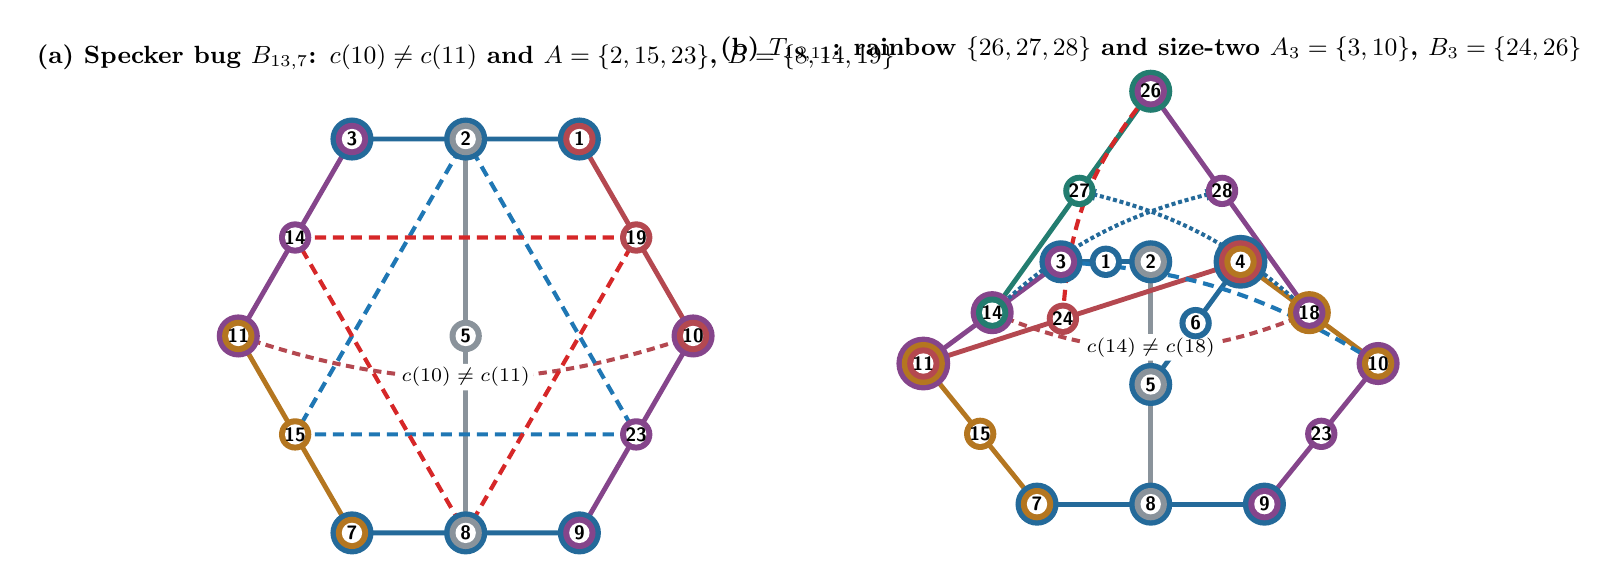
\begin{tikzpicture}[x=1cm,y=1cm]
  % --- Panel (a): Specker bug B_13,7 ---
  \begin{scope}[shift={(-4.35,0)},scale=0.76]
    \node[font=\bfseries\small] at (0,4.65) {(a) Specker bug $B_{13,7}$: $c(10)\neq c(11)$ and $A=\{2,15,23\}$, $B=\{8,14,19\}$};
    \def\R{3.8}
    \coordinate (v10) at (  0:\R);
    \coordinate (v1)  at ( 60:\R);
    \coordinate (v3)  at (120:\R);
    \coordinate (v11) at (180:\R);
    \coordinate (v7)  at (240:\R);
    \coordinate (v9)  at (300:\R);
    \coordinate (v2)  at ($(v3)!.5!(v1)$);
    \coordinate (v8)  at ($(v7)!.5!(v9)$);
    \coordinate (v5)  at (0,0);
    \coordinate (v14) at ($(v11)!.5!(v3)$);
    \coordinate (v15) at ($(v11)!.5!(v7)$);
    \coordinate (v19) at ($(v1)!.5!(v10)$);
    \coordinate (v23) at ($(v9)!.5!(v10)$);

    \draw[YOtrace,YOctx1]  (v3)--(v2)--(v1);
    \draw[YOtrace,YOctx2]  (v7)--(v8)--(v9);
    \draw[YOtrace,YOctx4]  (v2)--(v5)--(v8);
    \draw[YOtrace,YOctx8]  (v11)--(v14)--(v3);
    \draw[YOtrace,YOctx9]  (v11)--(v15)--(v7);
    \draw[YOtrace,YOctx11] (v9)--(v23)--(v10);
    \draw[YOtrace,YOctx12] (v1)--(v19)--(v10);

    % Sub-complete rainbow pair {10,11}
    \draw[CSexcl] (v11) to[bend right=18] node[CSnote,pos=.5] {$c(10)\neq c(11)$} (v10);
    % Highlight size-3 paired pseudocontexts A={2,15,23} (blue) and B={8,14,19} (red)
    \draw[CSmarkedA] (v2)--(v15)--(v23)--cycle;
    \draw[CSmarkedB] (v8)--(v14)--(v19)--cycle;

    \YOvertex{1}{1/.36,12/.27}
    \YOvertex{2}{1/.36,4/.27}
    \YOvertex{3}{1/.36,8/.27}
    \YOvertex{5}{4/.27}
    \YOvertex{7}{2/.36,9/.27}
    \YOvertex{8}{2/.36,4/.27}
    \YOvertex{9}{2/.36,11/.27}
    \YOvertex{10}{11/.36,12/.27}
    \YOvertex{11}{8/.36,9/.27}
    \YOvertex{14}{8/.27}
    \YOvertex{15}{9/.27}
    \YOvertex{19}{12/.27}
    \YOvertex{23}{11/.27}
  \end{scope}

  % --- Panel (b): Two-way gadget T_19,11 ---
  \begin{scope}[shift={(4.35,-0.35)},scale=0.76]
    \node[font=\bfseries\small] at (0,5.25) {(b) $T_{19,11}$: rainbow $\{26,27,28\}$ and size-two $A_3=\{3,10\}$, $B_3=\{24,26\}$};
    \coordinate (v11) at (-3.80, 0.00);
    \coordinate (v10) at ( 3.80, 0.00);
    \coordinate (v3)  at (-1.50, 1.70);
    \coordinate (v1)  at (-0.75, 1.70);
    \coordinate (v2)  at ( 0.00, 1.70);
    \coordinate (v4)  at ( 1.50, 1.70);
    \coordinate (v7)  at (-1.90,-2.35);
    \coordinate (v8)  at ( 0.00,-2.35);
    \coordinate (v9)  at ( 1.90,-2.35);
    \coordinate (v5)  at ( 0.00,-0.35);
    \coordinate (v6)  at ($(v5)!.5!(v4)$);
    \coordinate (v14) at ($(v11)!.5!(v3)$);
    \coordinate (v15) at ($(v11)!.5!(v7)$);
    \coordinate (v18) at ($(v10)!.5!(v4)$);
    \coordinate (v23) at ($(v9)!.5!(v10)$);
    \coordinate (v24) at ($(v11)!.44!(v4)$);
    \coordinate (v26) at ( 0.00, 4.55);
    \coordinate (v27) at ($(v14)!.55!(v26)$);
    \coordinate (v28) at ($(v18)!.55!(v26)$);

    \draw[YOtrace,YOctx1]  (v3)--(v1)--(v2);
    \draw[YOtrace,YOctx2]  (v7)--(v8)--(v9);
    \draw[YOtrace,YOctx3]  (v5)--(v6)--(v4);
    \draw[YOtrace,YOctx4]  (v2)--(v5)--(v8);
    \draw[YOtrace,YOctx8]  (v11)--(v14)--(v3);
    \draw[YOtrace,YOctx9]  (v11)--(v15)--(v7);
    \draw[YOtrace,YOctx11] (v9)--(v23)--(v10);
    \draw[YOtrace,YOctx13] (v10)--(v18)--(v4);
    \draw[YOtrace,YOctx10] (v11)--(v24)--(v4);
    \draw[YOtrace,YOctx5]  (v14)--(v27)--(v26);
    \draw[YOtrace,YOctx16] (v18)--(v28)--(v26);

    \draw[CSexcl]  (v14) to[bend right=22] node[CSnote,pos=.5] {$c(14)\neq c(18)$} (v18);
    \draw[CSident] (v14) to[bend left=14]  (v28);
    \draw[CSident] (v18) to[bend right=14] (v27);
    % Highlight size-2 pair {3,10} vs {24,26}
    \draw[CSmarkedA] (v3) to[bend left=14] (v10);
    \draw[CSmarkedB] (v24) to[bend left=18] (v26);

    \YOvertex{1}{1/.27}
    \YOvertex{2}{1/.36,4/.27}
    \YOvertex{3}{1/.36,8/.27}
    \YOvertex{4}{3/.45,10/.36,13/.27}
    \YOvertex{5}{3/.36,4/.27}
    \YOvertex{6}{3/.27}
    \YOvertex{7}{2/.36,9/.27}
    \YOvertex{8}{2/.36,4/.27}
    \YOvertex{9}{2/.36,11/.27}
    \YOvertex{10}{11/.36,13/.27}
    \YOvertex{11}{8/.45,9/.36,10/.27}
    \YOvertex{14}{8/.36,5/.27}
    \YOvertex{15}{9/.27}
    \YOvertex{18}{13/.36,16/.27}
    \YOvertex{23}{11/.27}
    \YOvertex{24}{10/.27}
    \YOvertex{26}{5/.36,16/.27}
    \YOvertex{27}{5/.27}
    \YOvertex{28}{16/.27}
  \end{scope}
\end{tikzpicture}%
}
\caption{Three-dimensional gadgets in $\R^3$ (coordinates in Table~\ref{tab:yo-vectors}): (a) Specker bug $B_{13,7}$ with universally rainbow pair $c(10)\neq c(11)$ and size-three affine pseudocontexts $A=\{2,15,23\}$ (blue dashed triangle) and $B=\{8,14,19\}$ (red dashed triangle); (b) $T_{19,11}$ with universally rainbow pair $c(14)\neq c(18)$, chromatic twins $14\sim_c 28$ and $18\sim_c 27$, complete rainbow tip triple $\{26,27,28\}$, and the non-twin color-multiset-equivalent pair $A_3=\{3,10\}$ (blue dashed arc) and $B_3=\{24,26\}$ (red dashed arc).}\label{fig:3d-gadgets}
\end{figure*}

\subsection{Chromatic Admissible Contexts in \texorpdfstring{$H_{20,12}$ and $H_{21,13}$}{H20,12 and H21,13}}\label{sec:H21-rainbow}

Finally, we turn to Class~I of Definition~\ref{def:chromatic-relations}: a single triple $U=\{u_1,u_2,u_3\}$ of \emph{pairwise nonorthogonal} rays in $\R^3$ ($q_{u_a}\not\perp q_{u_b}$ for all $a\neq b$) that is chromatically complete ($\{c(u_1),c(u_2),c(u_3)\}=\{0,1,2\}$) in \emph{every} strong $3$-coloring $c\in\Cc_3(H)$.

\begin{lemma}[Structural Color Propagation in $H_{21,13}$]\label{lem:H21-structural}
Every strong $3$-coloring gives distinct colors to the hubs $10,11,13$ and to each of the triples $\{1,4,7\}$ and $\{3,6,9\}$. There are exactly two normalized strong $3$-colorings, representing all $12$ labeled colorings.
\end{lemma}
\begin{proof}
Suppose first that hubs $10,11$ share color $t$. Vertices $1,3$ both avoid $t$, so their context forces $c(2)=t$. Similarly, vertices $7,9$ both avoid $t$, forcing $c(8)=t$, contrary to the context $\{2,5,8\}$. Equating hubs $10,13$ similarly forces $c(5)=c(8)$, while equating $11,13$ forces $c(2)=c(5)$. Thus the hub triple is rainbow.

Adjacency to two hubs now forces
\[
c(1)=c(11),\quad c(4)=c(13),\quad c(7)=c(10),
\]
so $\{1,4,7\}$ is rainbow. Arrange the three base contexts as rows of
\[
\begin{pmatrix}1&2&3\\4&5&6\\7&8&9\end{pmatrix}.
\]
Every row contains each color once. The first column is rainbow by the preceding argument, and the middle column is an actual context. Counting occurrences of each color therefore leaves exactly one occurrence in the last column, proving that $\{3,6,9\}$ is rainbow.

Normalize the middle column to $(0,1,2)$. The first column is a permutation avoiding the middle-column color in each row, so it is one of the two derangements of three colors. The last column, the hubs, and every remaining vertex are then uniquely determined. Both derangements extend to all contexts. Hence there are two normalized colorings, and their six color permutations exhaust all $12$ labeled strong colorings.
\end{proof}

\begin{theorem}[Sharp Minimality and Transversal Classification in Yu--Oh Restrictions]\label{thm:H21-complete}
Consider the $13$-context, $21$-ray Yu--Oh restriction $H_{21,13}$ in $\R^3$ (Table~\ref{tab:yo-vectors} and Fig.~\ref{fig:H21-admissibility}) obtained by omitting the single diagonal sector $h_0=12$ from $H_{\YO}^+$~\cite{svozil-2026-chromaticcoordinatization,2026-latin-context-matrix}.
\begin{enumerate}
\item \emph{Sharp threshold at $12$ contexts ($H_{20,12}$):} Among all $2^{13}=8{,}192$ context subhypergraphs of $H_{21,13}$, none with $|E|\le 11$ contexts possesses a pairwise-nonorthogonal complete rainbow triple. At $|E|=12$, deleting a single roof context from one diagonal sector---for instance omitting $\{6,13,22\}$ to form $H_{20,12}$ ($|V|=20$, $|E|=12$, $N_c=4$, $|\Sc_{\mathrm{ext}}|/|\Sc|=10/25$)---yields the minimal configuration, which already forces two pairwise-nonorthogonal complete rainbow triples:
\begin{equation}\label{eq:H20-triples}
U_1^{(20)}=\{15,18,20\},\qquad U_2^{(20)}=\{19,21,24\}.
\end{equation}
\item \emph{Even-transversal classification in $H_{21,13}$ ($|V|=21$, $|E|=13$, $N_c=2$, $|\Sc_{\mathrm{ext}}|/|\Sc|=6/21$):} Each vertex $v\in V(H_{21,13})$ has a bivariate color signature $\sigma(v)=(c_1(v),c_2(v))\in\{0,1,2\}^2$ across the two normalized $13\times 3$ Context--Color Matrices [Eq.~(16) of Ref.~\cite{2026-latin-context-matrix}], partitioning $V(H_{21,13})$ into the $3\times 3$ signature grid:
\begin{equation}\label{eq:H21-signature-grid}
\begin{array}{c|ccc}
c_2\backslash c_1 & \mathbf{c}_0=0 & \mathbf{c}_1=1 & \mathbf{c}_2=2\\\hline
0 & \{2,14\} & \{6\} & \{7,10,20,24\}\\
1 & \{4,13,15,19\} & \{8,23\} & \{3\}\\
2 & \{9\} & \{1,11,18,21\} & \{5,22\}
\end{array}
\end{equation}
A triple $U\subseteq V(H_{21,13})$ is rainbow in every $3$-coloring if and only if $U$ is a \emph{permutation transversal}~\cite{wanless2011transversals} of Eq.~\eqref{eq:H21-signature-grid}, selecting one vertex from each row and one from each column ($\sum_{\pi\in S_3}\prod_{i=0}^2 |F_{i,\pi(i)}|=97$ total transversals, i.e., $13$ contexts plus $84$ non-context rainbow triples). The three odd permutations $\pi\in S_3$ contain $0$ pairwise-nonorthogonal triples, whereas the three even (cyclic) permutations yield \emph{exactly $21$ chromatic admissible contexts}:
\begin{itemize}
\item \emph{Singleton cyclic transversal $F_{0,2}\times F_{1,0}\times F_{2,1}$ ($1$ triple):}
\begin{equation}\label{eq:U-369}
U_{\mathrm{cop}}=\{3,6,9\},
\end{equation}
whose rays $r_3=(0,1,-1)$, $r_6=(1,-1,0)$, $r_9=(1,0,-1)$ are not only pairwise nonorthogonal ($\ip{r_3}{r_6}=-1$, $\ip{r_3}{r_9}=1$, $\ip{r_6}{r_9}=1$) but \emph{coplanar} ($r_3+r_6-r_9=\mathbf{0}$, spanning the plane orthogonal to omitted hub $r_{12}=(1,1,1)$ so $\rank(P_3+P_6+P_9)=2<3$).
\item \emph{Main diagonal transversal $F_{0,0}\times F_{1,1}\times F_{2,2}$ ($4$ of $8$ triples):}
\begin{equation}\label{eq:U-diag1}
\{2,22,23\},\quad \{5,14,23\},\quad \{8,14,22\},\quad \{14,22,23\}.
\end{equation}
\item \emph{Cyclic transversal $F_{0,1}\times F_{1,2}\times F_{2,0}$ ($16$ of $64$ triples):}
\begin{equation}\label{eq:U-diag2}
\begin{aligned}
&\{1,4,7\},\ \{1,15,24\},\ \{4,20,21\},\ \{7,18,19\},\\
&\{10,11,13\},\ \{10,15,21\},\ \{11,19,20\},\ \{13,18,24\},\\
&\{15,18,20\},\ \{15,18,24\},\ \{15,20,21\},\ \{15,21,24\},\\
&\{18,19,20\},\ \{18,19,24\},\ \{19,20,21\},\ \{19,21,24\}.
\end{aligned}
\end{equation}
In particular, $U_{\mathrm{core}}=\{1,4,7\}$ consists of three core rays $r_1=(0,1,1)$, $r_4=(1,1,0)$, $r_7=(1,0,1)$ at pairwise $60^\circ$, and $U_{\mathrm{hub}}=\{10,11,13\}$ consists of the three retained diagonal hubs $r_{10}=(1,-1,1)$, $r_{11}=(1,-1,-1)$, $r_{13}=(1,1,-1)$.
\end{itemize}
\item \emph{Chromatic twin classes of size four ($k=4>d=3$):} All four rays within each of the three $4$-element signature fibers $F_{0,2}=\{7,10,20,24\}$, $F_{1,0}=\{4,13,15,19\}$, and $F_{2,1}=\{1,11,18,21\}$ of Eq.~\eqref{eq:H21-signature-grid} are pairwise nonorthogonal in $\R^3$ and share the exact same color in every $3$-coloring of $H_{21,13}$.
\end{enumerate}
\end{theorem}
\begin{proof}
By Lemma~\ref{lem:H21-structural}, any strong $3$-coloring $c\in\Cc_3(H_{21,13})$ is obtained by applying a color permutation $\tau\in S_3$ to either $c_1$ or $c_2$. Hence $\{c(u_1),c(u_2),c(u_3)\}=\{0,1,2\}$ holds for all $c\in\Cc_3(H_{21,13})$ iff $\{c_1(u_1),c_1(u_2),c_1(u_3)\}=\{0,1,2\}$ and $\{c_2(u_1),c_2(u_2),c_2(u_3)\}=\{0,1,2\}$, meaning that the three signatures $\sigma(u_1),\sigma(u_2),\sigma(u_3)$ have distinct first coordinates and distinct second coordinates---the definition of a permutation transversal of Eq.~\eqref{eq:H21-signature-grid}. Exact inner-product checks on the $97$ transversals give the listed geometric classification and twin classes. Part~(1) is a computer-assisted minimality result: all $2^{13}$ context subhypergraphs were enumerated, their strong colorings computed, and their independent complete triples tested. The elementary universal-completeness and coloring-count arguments are supplied separately by Lemma~\ref{lem:H21-structural}.
\end{proof}

Over all $21$ ordinary two-valued states $s\in\Sc(H_{21,13})$, the sum $s(u_1)+s(u_2)+s(u_3)$ on $U_{\mathrm{core}}=\{1,4,7\}$ takes values $0,1,2$ with multiplicities $6,12,3$, and on $U_{\mathrm{cop}}=\{3,6,9\}$ takes values $0,1,2$ with multiplicities $3,12,6$; on the $6$ extendable states $\Sc_{\mathrm{ext}}(H_{21,13})$ it is identically $1$.

\begin{figure}[!htbp]
\centering
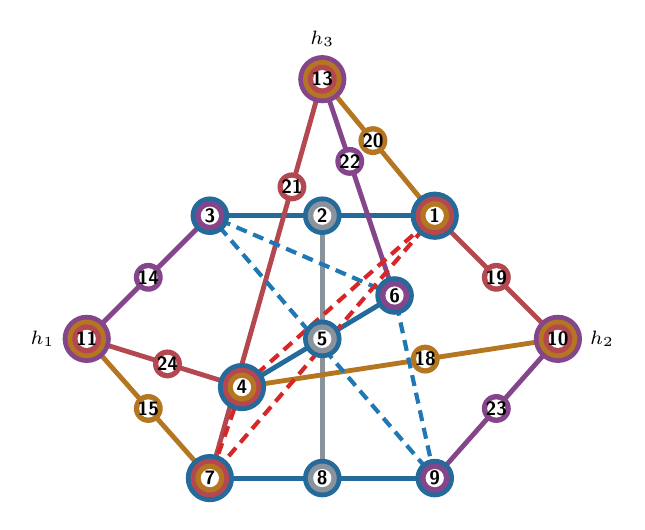
\begin{tikzpicture}[x=1cm,y=1cm,scale=0.68]
  \coordinate (v11) at (-4.40, 0.00);
  \coordinate (v10) at ( 4.40, 0.00);
  \coordinate (v3)  at (-2.10, 2.30);
  \coordinate (v2)  at ( 0.00, 2.30);
  \coordinate (v1)  at ( 2.10, 2.30);
  \coordinate (v7)  at (-2.10,-2.60);
  \coordinate (v8)  at ( 0.00,-2.60);
  \coordinate (v9)  at ( 2.10,-2.60);
  \coordinate (v5)  at ( 0.00, 0.00);
  \coordinate (v14) at ($(v11)!.5!(v3)$);
  \coordinate (v15) at ($(v11)!.5!(v7)$);
  \coordinate (v19) at ($(v1)!.5!(v10)$);
  \coordinate (v23) at ($(v9)!.5!(v10)$);
  \coordinate (v4)  at (-1.50,-0.90);
  \coordinate (v6)  at ( 1.35, 0.81);
  \coordinate (v24) at ($(v11)!.52!(v4)$);
  \coordinate (v18) at ($(v10)!.42!(v4)$);
  \coordinate (v13) at ( 0.00, 4.85);
  \coordinate (v20) at ($(v13)!.45!(v1)$);
  \coordinate (v22) at ($(v13)!.38!(v6)$);
  \coordinate (v21) at ($(v13)!.27!(v7)$);

  % 13 straight-line contexts
  \draw[YOtrace,YOctx1]  (v3)--(v2)--(v1);
  \draw[YOtrace,YOctx2]  (v7)--(v8)--(v9);
  \draw[YOtrace,YOctx3]  (v4)--(v5)--(v6);
  \draw[YOtrace,YOctx4]  (v2)--(v5)--(v8);
  \draw[YOtrace,YOctx8]  (v11)--(v14)--(v3);
  \draw[YOtrace,YOctx9]  (v11)--(v15)--(v7);
  \draw[YOtrace,YOctx11] (v9)--(v23)--(v10);
  \draw[YOtrace,YOctx12] (v1)--(v19)--(v10);
  \draw[YOtrace,YOctx10] (v11)--(v24)--(v4);
  \draw[YOtrace,YOctx13] (v10)--(v18)--(v4);
  \draw[YOtrace,YOctx16] (v6)--(v22)--(v13);
  \draw[YOtrace,YOctx14] (v13)--(v20)--(v1);
  \draw[YOtrace,YOctx15] (v13)--(v21)--(v7);

  % Highlight Chromatic Admissible Contexts U_cop={3,6,9} (blue dashed) and U_core={1,4,7} (red dashed)
  \draw[CSmarkedA] (v3)--(v6)--(v9)--cycle;
  \draw[CSmarkedB] (v1)--(v4)--(v7)--cycle;

  \YOvertex{1}{1/.45,12/.36,14/.27}
  \YOvertex{2}{1/.36,4/.27}
  \YOvertex{3}{1/.36,8/.27}
  \YOvertex{4}{3/.45,10/.36,13/.27}
  \YOvertex{5}{3/.36,4/.27}
  \YOvertex{6}{3/.36,16/.27}
  \YOvertex{7}{2/.45,15/.36,9/.27}
  \YOvertex{8}{2/.36,4/.27}
  \YOvertex{9}{2/.36,11/.27}
  \YOvertex{10}{11/.45,13/.36,12/.27}
  \YOvertex{11}{8/.45,9/.36,10/.27}
  \YOvertex{13}{16/.45,14/.36,15/.27}
  \YOvertex{14}{8/.27}
  \YOvertex{15}{9/.27}
  \YOvertex{18}{13/.27}
  \YOvertex{19}{12/.27}
  \YOvertex{20}{14/.27}
  \YOvertex{21}{15/.27}
  \YOvertex{22}{16/.27}
  \YOvertex{23}{11/.27}
  \YOvertex{24}{10/.27}

  \node[YOlabel,left=3pt]  at ($(v11)+(-.38,0)$) {$h_1$};
  \node[YOlabel,right=3pt] at ($(v10)+(.38,0)$)  {$h_2$};
  \node[YOlabel,above=3pt] at ($(v13)+(0,.38)$)  {$h_3$};
\end{tikzpicture}
\caption{The $21$-ray, $13$-context Yu--Oh restriction $H_{21,13}$ in $\R^3$ (all $13$ contexts drawn as straight lines; coordinates in Table~\ref{tab:yo-vectors}). Highlighted are two of the $21$ chromatic admissible contexts (Theorem~\ref{thm:H21-complete}): the coplanar triple $U_{\mathrm{cop}}=\{3,6,9\}$ (blue dashed triangle, $r_3+r_6-r_9=\mathbf{0}$) and the $60^\circ$ basis triple $U_{\mathrm{core}}=\{1,4,7\}$ (red dashed triangle), both satisfying $\{c(u_1),c(u_2),c(u_3)\}=\{0,1,2\}$ in every $3$-coloring of $H_{21,13}$.}\label{fig:H21-admissibility}
\end{figure}

\subsection{Color-Weighted Quantum Maxima for the Chromatic Targets}\label{sec:weighted-YO}

For each ordered rainbow triple in Table~\ref{tab:weighted-YO}, choose color labels so that its three weights are $(c_0,c_1,c_2)$. The table gives an exact parameterized eigensystem through Eqs.~\eqref{eq:weighted-triple-coefficients}--\eqref{eq:weighted-cubic-maximum}: its maximal expectation is $F(c_0+c_1+c_2,b,gc_0c_1c_2)$, where $b=h_{01}c_0c_1+h_{02}c_0c_2+h_{12}c_1c_2$. The $H_{20,12}$ rows use the separate faithful coordinates specified in Table~\ref{tab:yo-vectors}, rather than the coordinates of $H_{21,13}$.

\begin{table}[t]
\caption{Exact characteristic-polynomial coefficients for representative ordered chromatic admissible triples. The same Gram-minor construction gives the coefficients of every other triple in Eqs.~\eqref{eq:U-diag1}--\eqref{eq:U-diag2}.}\label{tab:weighted-YO}
\footnotesize\setlength{\tabcolsep}{3pt}
\begin{ruledtabular}
\begin{tabular}{lcccc}
Ordered triple & $h_{01}$ & $h_{02}$ & $h_{12}$ & $g$\\\hline
$H_{21,13}$: $(1,4,7)$ & $3/4$ & $3/4$ & $3/4$ & $1/2$\\
$H_{21,13}$: $(3,6,9)$ & $3/4$ & $3/4$ & $3/4$ & $0$\\
$H_{21,13}$: $(10,11,13)$ & $8/9$ & $8/9$ & $8/9$ & $16/27$\\
$H_{20,12}$: $(15,18,20)$ & $131/135$ & $1573/1575$ & $913/945$ & $529/567$\\
$H_{20,12}$: $(19,21,24)$ & $4469/4725$ & $134/135$ & $314/315$ & $529/567$
\end{tabular}
\end{ruledtabular}
\end{table}

For the core and coplanar triples, the operators themselves are particularly transparent:
\begin{equation}\label{eq:weighted-YO-operators}
\begin{aligned}
O_{\mathrm{core}}&=\frac12\begin{pmatrix}
c_1+c_2&c_1&c_2\\c_1&c_0+c_1&c_0\\c_2&c_0&c_0+c_2
\end{pmatrix},\\
O_{\mathrm{cop}}&=\frac12\begin{pmatrix}
c_1+c_2&-c_1&-c_2\\-c_1&c_0+c_1&-c_0\\-c_2&-c_0&c_0+c_2
\end{pmatrix}.
\end{aligned}
\end{equation}
Writing $t=c_0+c_1+c_2$ and $b=\tfrac34(c_0c_1+c_0c_2+c_1c_2)$, the coplanar eigensystem has the fixed zero eigenvector $(1,1,1)^{\mathsf T}/\sqrt3$ and two remaining eigenvalues
\begin{equation}\label{eq:weighted-coplanar-max}
\begin{aligned}
\lambda_\pm&=\tfrac12\left(t\pm\sqrt{t^2-4b}\right),\\
\max_\rho\bigl[c_0p_\rho(3)+c_1p_\rho(6)+c_2p_\rho(9)\bigr]
&=\max\{0,\lambda_+\}.
\end{aligned}
\end{equation}
The other eigenspaces are obtained from Eq.~\eqref{eq:weighted-spectral-resolution}. This formula includes negative color values, for which the fixed zero eigenvalue can be the maximum.

At $\mathbf c=\mathbf1$, put $n=(1,1,1)^{\mathsf T}/\sqrt3$. Then
\begin{equation}\label{eq:weighted-YO-unit-eigensystems}
\begin{aligned}
O_{\mathrm{core}}&=2nn^{\mathsf T}+\tfrac12(I_3-nn^{\mathsf T}),\\
O_{\mathrm{cop}}&=\tfrac32(I_3-nn^{\mathsf T}),\\
O_{\mathrm{hub}}&=\tfrac13nn^{\mathsf T}+\tfrac43(I_3-nn^{\mathsf T}).
\end{aligned}
\end{equation}
Their maxima are therefore $2$, $3/2$, and $4/3$, respectively. The maximizing preparations are $n$ for the core and any unit vector in $n^\perp$ for the other two. These are quantum maxima for the fixed FOR; the normalization value one on extendable states remains a separate statement.

The smaller chromatic relations have explicit two-ray eigensystems as well. For any ordered pair of distinct rays $(u,v)$, put $a=c_{\kappa(u)}$, $b=c_{\kappa(v)}$, and $r=|\ip{\hat q_u}{\hat q_v}|^2$. In $\C^3$,
\begin{equation}\label{eq:weighted-two-ray-spectrum}
\operatorname{spec}(aP_u+bP_v)
=\left\{0,\frac{a+b\pm\sqrt{(a-b)^2+4abr}}2\right\}.
\end{equation}
Thus its maximum is the larger of zero and the plus branch. For a chromatic twin pair, $a=b$ and the nonzero branches are $a(1\pm\sqrt r)$. For the non-twin paired sets in Section~\ref{sec:size2-real}, use Eq.~\eqref{eq:weighted-pair-difference}; their difference is traceless by color-multiset equivalence, and Eq.~\eqref{eq:weighted-pair-cubic} gives its exact maximum. This applies to a fixed coloring and its actual color weights, without promoting a chromatic relation to an affine certificate.

\subsection{Classical Comparisons for the Logical and Yu--Oh Targets}\label{sec:classical-YO}

The two independent triples of $H_{20,12}$ have the seven nonzero binary restrictions on their $25$ two-valued states. For either ordered triple, with colors normalized to $(0,1,2)$, the sharp full-state bounds are the minimum and maximum of
\begin{equation}\label{eq:classical-H20-envelope}
\{c_0,c_1,c_2,c_0+c_1,c_0+c_2,c_1+c_2,c_0+c_1+c_2\}.
\end{equation}
On the ten extendable states the bounds instead come from $\{c_0,c_1,c_2\}$. At unit values, both triples have full classical interval $[1,3]$ and quantum interval approximately $[0.72960967,1.23483806]$ in the stated faithful representation. The quantum minimum therefore violates the full classical lower bound; the quantum maximum exceeds one only relative to the extendable-state normalization.

For $H_{21,13}$, each of the core and coplanar triples has all binary restrictions except $(1,1,1)$. Their exact full classical envelope is Eq.~\eqref{eq:classical-M15-single}. Thus their unit quantum intervals, $[1/2,2]$ and $[0,3/2]$, are contained in the full classical interval $[0,2]$. In fact no choice of real color values on either of these triples separates all two-valued states: their classical projected polytope is
\[
\{x\in[0,1]^3:x_0+x_1+x_2\le2\},
\]
and every Born probability vector lies in it, by the displayed spectral upper bounds and $0\le p_\rho(v)\le1$.

The hub triple behaves differently. Its full-state restrictions are $000,100,010,001$, giving
\begin{equation}\label{eq:classical-hub-envelope}
\begin{aligned}
\beta^-_{\Sc}(\mathbf c)&=\min\{0,c_0,c_1,c_2\},\\
\beta^+_{\Sc}(\mathbf c)&=\max\{0,c_0,c_1,c_2\}.
\end{aligned}
\end{equation}
At unit values its full classical interval is $[0,1]$, whereas its quantum maximum is $4/3$. An explicit maximizing preparation is
\begin{equation}\label{eq:H21-hub-explicit-witness}
\begin{aligned}
\psi_{\mathrm{hub}}&=(1,-1,0)^{\mathsf T}/\sqrt2,\\
\bigl(p_{\psi_{\mathrm{hub}}}(10),p_{\psi_{\mathrm{hub}}}(11),p_{\psi_{\mathrm{hub}}}(13)\bigr)
&=(2/3,2/3,0).
\end{aligned}
\end{equation}
Thus the classical inequality $p(10)+p(11)+p(13)\le1$ is violated on an exact preparation. Its bound holds on all two-valued states, not only on the six extendable states.

The same calculation distinguishes the smaller logical gadgets. The pair $\{14,18\}$ in $D_{16,9}$ has all four binary restrictions on $\Sc$, but only $00,10,01$ on $\Sc_{\mathrm{ext}}$. Its quantum unit maximum $49/45$ therefore exceeds the extendable bound one while remaining within the full bound two. In $I_{16,9}$ and $H_{17,10}$, the original bug tips $\{10,11\}$ are exclusive on all two-valued states, and their quantum maxima are approximately $1.27216553$ and $4/3$, respectively. The first value uses the integer FOR for panel~(d) in the companion's vector inventory~\cite{supplement}, explicitly included in the computational inventory; the graph's state space does not change when the FOR is changed. In $T_{19,11}$, the pair $\{9,26\}$ is exclusive on all $25$ two-valued states and has quantum maximum $1.25241492$, even though the particular relation $\{14,18\}$ is purely chromatic. The complete comparison retains every counted rainbow pair, twin difference, and paired relation, so these representative comparisons do not replace the full inventory.

\subsection{Two-Valued Admissibility Contexts in \texorpdfstring{$\R^3$}{R3}}\label{sec:tvs-admissibility}

Can an independent triple be normalized on \emph{every} two-valued state of a faithfully represented, $3$-colorable hypergraph in $\R^3$? The answer is affirmative. The mechanism below has two separate ingredients: a binary implication across two contexts, and a geometric realization of the gadgets supplying its exclusivity assumptions. Figure~\ref{fig:TVS-admissibility} displays the implication in two stages.

\begin{lemma}[Roof Twins]\label{lem:roof-twin}
Let $H$ contain the contexts $\{a,x,y'\}$ and $\{a,y,x'\}$. Suppose
\begin{equation}\label{eq:roof-excl}
s(x)+s(y)\le1,\qquad s(x')+s(y')\le1
\end{equation}
for every $s\in\Sc(H)$. Then every such state satisfies
\begin{equation}\label{eq:roof-twins}
s(x)=s(x'),\qquad s(y)=s(y'),
\end{equation}
and consequently
\begin{equation}\label{eq:roof-sum1}
\begin{aligned}
s(a)+s(x)+s(y)&=1,\\
s(a)+s(x')+s(y')&=1.
\end{aligned}
\end{equation}
\end{lemma}
\begin{proof}
Subtracting the two context equations gives
\[
\delta=s(x)-s(x')=s(y)-s(y')\in\{-1,0,1\}.
\]
If $\delta=1$, then $s(x)=s(y)=1$; if $\delta=-1$, then $s(x')=s(y')=1$. Both contradict Eq.~\eqref{eq:roof-excl}. Hence $\delta=0$, proving the twin identities. Substitution into either context equation gives Eq.~\eqref{eq:roof-sum1}. This step uses the binary range of $s$.
\end{proof}

Write $B(x,y;\ell)$ for a Specker bug with tips $x,y$ and eleven new vertices $\ell+k$, where $k\in\{1,2,3,5,7,8,9,14,15,19,23\}$. Its seven contexts are
\begin{equation}\label{eq:roof-bug-contexts}
\begin{gathered}
\{\ell+1,\ell+2,\ell+3\},\quad
\{\ell+7,\ell+8,\ell+9\},\\
\{\ell+2,\ell+8,\ell+5\},\\
\{\ell+3,y,\ell+14\},\quad
\{\ell+7,y,\ell+15\},\\
\{\ell+9,x,\ell+23\},\quad
\{\ell+1,x,\ell+19\}.
\end{gathered}
\end{equation}
These contexts force $s(x)+s(y)\le1$: if both tips were one, vertices $\ell+1,\ell+3,\ell+7,\ell+9$ would be zero, so the first two contexts would force $s(\ell+2)=s(\ell+8)=1$, contradicting the third context. This is the only bug implication needed for the cascade.

\begin{lemma}[Specker-Bug Coordinates]\label{lem:bug-triad}
Let $u,v\in\R^3$ have equal nonzero norm and
$0<\ip{\hat u}{\hat v}\le1/3$, after reversing one vector if necessary. Set $e_1=u+v$, $e_2=u-v$, $e_3=u\times v$, and
\begin{equation}\label{eq:universal-phi}
\cos\phi=\sqrt{2-\frac{\|e_1\|^2}{\|e_2\|^2}},\qquad
\sin\phi=\sqrt{\frac{\|e_1\|^2}{\|e_2\|^2}-1}.
\end{equation}
The orthonormal triad
\begin{equation}\label{eq:universal-triad}
\begin{aligned}
f_{1,2}&=\tfrac1{\sqrt2}\bigl(\hat e_1\pm
 (\cos\phi\,\hat e_2+\sin\phi\,\hat e_3)\bigr),\\
f_3&=f_1\times f_2
\end{aligned}
\end{equation}
gives the intended orthogonalities of Eq.~\eqref{eq:roof-bug-contexts}. Explicitly, with $r_x=u$, $r_y=v$ and $q_k=r_{\ell+k}$, take
\begin{equation}\label{eq:roof-bug-rays}
\begin{aligned}
q_2&=f_1,& q_8&=f_2,&q_5&=f_3,\\
q_1&=f_1\times u,&q_3&=f_1\times v,\\
q_9&=f_2\times u,&q_7&=f_2\times v,\\
q_{14}&=v\times q_3,&q_{15}&=v\times q_7,\\
q_{19}&=u\times q_1,&q_{23}&=u\times q_9.
\end{aligned}
\end{equation}
Faithfulness of a compound hypergraph additionally requires checking that all its rays are distinct and that no orthogonal pair is absent from its two-section graph.
\end{lemma}
\begin{proof}
The overlap bound makes both square roots real. The vectors $e_1,e_2,e_3$ are mutually orthogonal, so $f_1,f_2,f_3$ are orthonormal. Lagrange's identity gives
\[
(f_i\times u)\cdot(f_i\times v)
=u\cdot v-(f_i\cdot u)(f_i\cdot v)=0,
\]
because
\[
(f_i\cdot u)(f_i\cdot v)
=\tfrac18(\|e_1\|^2-\cos^2\phi\,\|e_2\|^2)
=u\cdot v.
\]
Thus $q_1\perp q_3$ and $q_7\perp q_9$; all remaining required orthogonalities follow directly from the cross products in Eq.~\eqref{eq:roof-bug-rays}.
\end{proof}

\begin{theorem}[Roof-Twin Cascades in $\R^3$]\label{thm:tvs-admissibility}
Starting from the nine-context hypergraph $I_{16,9}$, define
\begin{align*}
G_{27,16}&=I_{16,9}\cup B(18,24;100),\\
G_{41,25}&=G_{27,16}\cup\{\{14,27,26\},\{18,28,26\}\}\\
&\hspace{3.5em}\cup B(27,28;200),\\
G_{41,26}&=G_{41,25}\cup\{\{4,5,105\}\}.
\end{align*}
All three admit FORs in $\R^3$ and strong $3$-colorings. Their respective values of $(N_c,|\Sc_{\mathrm{ext}}|,|\Sc|)$ are
$(36,54,82)$, $(216,216,396)$, and $(48,63,107)$.
Every two-valued state of $G_{27,16}$ satisfies $s(11)=s(18)$ and $s(10)=s(24)$. In each of the two $41$-ray hypergraphs, every two-valued state satisfies
\begin{equation}\label{eq:G41-twins}
\begin{gathered}
s(11)=s(18)=s(27),\qquad s(14)=s(28),\\
s(3)=s(26).
\end{gathered}
\end{equation}
In particular,
\begin{equation}\label{eq:U-TVS}
\begin{gathered}
U_{\mathrm{TVS}}=\{3,27,28\},\\
s(3)+s(27)+s(28)=1\qquad(\forall s\in\Sc)
\end{gathered}
\end{equation}
is a pairwise-nonorthogonal two-valued state admissibility context in both $G_{41,25}$ and $G_{41,26}$.
\end{theorem}
\begin{proof}
\emph{Binary implication.} The original bug $B(10,11;0)$ and the attached $B(18,24;100)$ supply the two exclusivity assumptions for the roof contexts $\{4,11,24\}$ and $\{4,10,18\}$. Lemma~\ref{lem:roof-twin} gives $s(11)=s(18)$ and $s(10)=s(24)$. Context $E_8=\{3,11,14\}$ therefore yields
\begin{equation}\label{eq:roof-inherited}
s(3)+s(14)+s(18)=1,
\end{equation}
so $s(14)+s(18)\le1$. The third bug supplies $s(27)+s(28)\le1$. Applying the same lemma to $\{26,14,27\}$ and $\{26,18,28\}$ gives $s(14)=s(28)$ and $s(18)=s(27)$. Substitution into Eq.~\eqref{eq:roof-inherited} proves Eq.~\eqref{eq:U-TVS}; comparison with either second-roof context also gives $s(3)=s(26)$. Adding a context only restricts the state space, so these implications hold for both $41$-ray cases. This proves universal normalization without enumerating states.

\emph{Faithful coordinates.} Geometric realizations must be distinguished from the preceding binary argument. A parametrization of $I_{16,9}$ is
\begin{equation}\label{eq:roof-base-rays}
\begin{aligned}
r_1&=(0,1,\alpha),&r_2&=(1,0,0),\\
r_3&=(0,\alpha,-1),&r_5&=(0,0,1),\\
r_7&=(1,0,\beta),&r_8&=(0,1,0),\\
r_9&=(\beta,0,-1),&r_{10}&=(1,-\alpha\beta,\beta),\\
r_{11}&=(\alpha\beta,-1,-\alpha),&r_4&=r_{10}\times r_{11},\\
r_{14}&=r_{11}\times r_3,&r_{15}&=r_7\times r_{11},\\
r_{19}&=r_1\times r_{10},&r_{23}&=r_{10}\times r_9,\\
r_{18}&=r_4\times r_{10},&r_{24}&=r_{11}\times r_4.
\end{aligned}
\end{equation}
At $(\alpha,\beta)=(9/32,24/11)$,
\begin{equation}\label{eq:r4-norm-factorization}
\begin{aligned}
\|r_4\|^2&=(1+\alpha^2)(1+\beta^2)(1+\alpha^2\beta^2),\\
\|r_4\|&=45305/15488.
\end{aligned}
\end{equation}
Put $n=r_4/\|r_4\|$ and $R=nn^{\mathsf T}-[n]_\times$, where $[n]_\times w=n\times w$. This is a quarter-turn about $n$. Both tips lie in $n^\perp$, where $Rw=-n\times w$, so it sends the rays of $r_{10},r_{11}$ to those of $r_{18},r_{24}$, respectively. Assigning $r_{100+k}=Rr_k$ for the eleven internal bug labels in Eq.~\eqref{eq:roof-bug-contexts} gives a rational FOR of $G_{27,16}$ (and integer representatives after rescaling).

At these same rational parameters, take $r_{26}=r_{14}\times r_{18}$, $r_{27}=r_{26}\times r_{14}$, $r_{28}=r_{26}\times r_{18}$ and apply Lemma~\ref{lem:bug-triad} to the last two rays. Their squared normalized overlap is
\[
\frac{21159411204096}{3980389958002705}<\frac19.
\]
This gives a FOR of $G_{41,25}$. The rotation and cross-product formulas establish all intended orthogonalities algebraically; outward-rounded interval evaluation at $70$ decimal digits certifies every other inner product to be nonzero and every pair of rays to be distinct. The smallest certified absolute normalized nonedge inner product exceeds $0.00155$.

For $G_{41,26}$, a simpler, separate realization uses $\alpha=\beta=1$. Choose the ray representatives $r_4=(1,1,0)$, $r_{14}=(2,1,1)$, $r_{18}=(1,-1,-2)$, $r_{24}=(1,-1,2)$. For the second bug use Eq.~\eqref{eq:roof-bug-rays} with $f_1=(1,1,\sqrt2)$, $f_2=(1,1,-\sqrt2)$ (normalization is immaterial for rays). For the second roof use
\begin{equation}\label{eq:G41-vectors}
\begin{aligned}
r_{26}&=(-1,5,-3),\\
r_{27}&=(8,-5,-11),\\
r_{28}&=(-13,-5,-4).
\end{aligned}
\end{equation}
Their normalized overlap has magnitude $1/6$. For the third bug, Eq.~\eqref{eq:roof-bug-rays} applies with
\begin{equation}\label{eq:roof-third-triad}
\begin{aligned}
f_{1,2}={}&\sqrt{35}\,(3,0,-1)\\
&\quad\pm\bigl(\sqrt{15}\,(1,2,3)+2(-1,5,-3)\bigr).
\end{aligned}
\end{equation}
Exact arithmetic in $\Q(\sqrt2,\sqrt{15},\sqrt{35})$ verifies all $820$ ray pairs: rays are distinct, and orthogonality is precisely adjacency in $G_{41,26}$. In particular,
\[
r_3\cdot r_{27}=6,\quad r_3\cdot r_{28}=-1,\quad
r_{27}\cdot r_{28}=-35,
\]
so the target triple is pairwise nonorthogonal. At these symmetric parameters, deleting $\{4,5,105\}$ leaves three unrecorded orthogonal pairs, namely $(4,5),(4,105),(5,105)$. Thus these symmetric coordinates are faithful for $G_{41,26}$, whereas $G_{27,16}$ and $G_{41,25}$ use the separate rational-parameter construction above.

\emph{Finite counts.} Exhaustive enumeration, independently checked by a second implementation, gives the stated state and normalized-coloring counts. The coordinate and state certificate supplies the full contexts, ray coordinates, assignments, and verification routines. Enumeration certifies the counts and geometry; the two applications of Lemma~\ref{lem:roof-twin} establish normalization on \emph{all} two-valued states.
\end{proof}

The separation from affine and operator normalization can be seen directly. In the symmetric FOR of $G_{41,26}$, prepare $\psi=\hat r_3=(0,1,-1)/\sqrt2$. Since $\|r_{27}\|^2=\|r_{28}\|^2=210$, its Born probabilities give
\begin{equation}\label{eq:roof-born-witness}
\begin{aligned}
p_\psi(3)+p_\psi(27)+p_\psi(28)
&=1+\frac{36}{420}+\frac1{420}\\
&=\frac{457}{420}\ne1.
\end{aligned}
\end{equation}
This weight lies in $\Wc(G_{41,26})\subset\mathcal A(G_{41,26})$, while every convex combination of two-valued states has target sum one. Hence $\operatorname{aff}\Sc(G_{41,26})\subsetneq\mathcal A(G_{41,26})$ and $P_3+P_{27}+P_{28}\ne I_3$, in agreement with Proposition~\ref{prop:no-operator-complete}. The uniform weight $p(v)=1/3$ satisfies the target normalization and every twin identity; it is not a separating witness. Indeed, any strong $3$-coloring expresses it as the average of its three color-class states.

\begin{figure*}[!t]
\centering
\resizebox{\textwidth}{!}{%
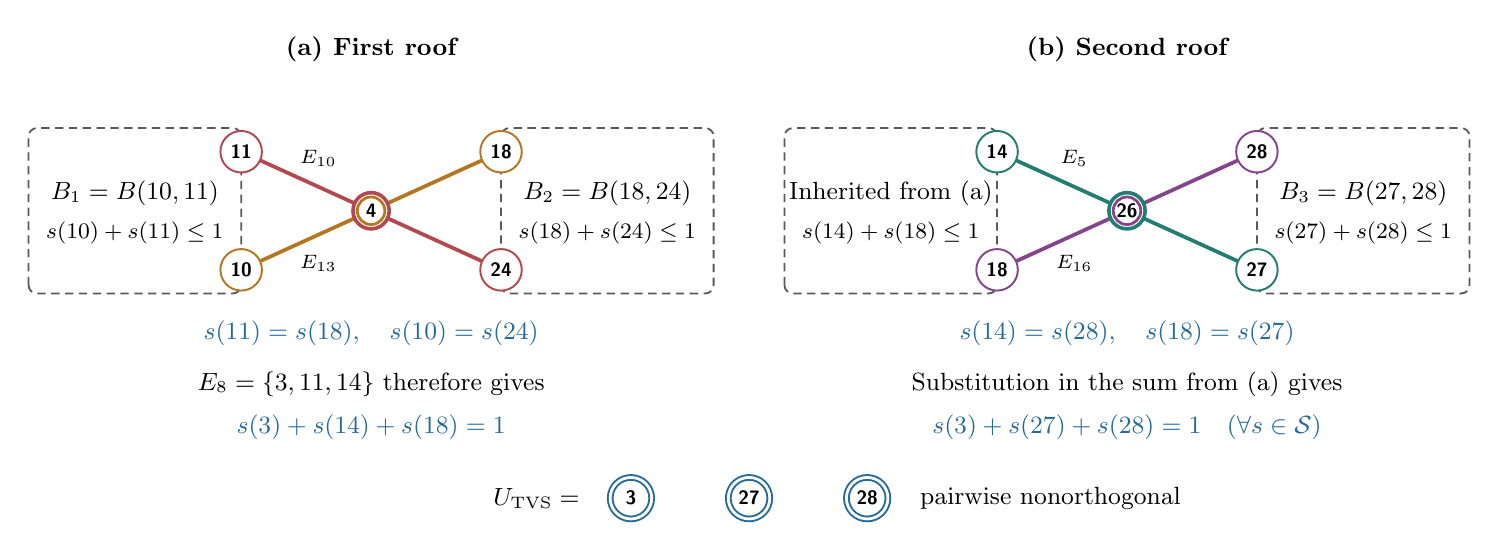
\begin{tikzpicture}[x=1cm,y=1cm,
  rooftrace/.style={line width=1.35pt,line cap=round},
  roofbox/.style={draw=black!65,densely dashed,line width=.65pt,rounded corners=3pt},
  roofnumber/.style={circle,draw=black,fill=white,line width=.7pt,
    minimum size=15pt,inner sep=0pt,font=\sffamily\bfseries\scriptsize},
  rooftext/.style={font=\small,align=center},
  roofresult/.style={font=\small,align=center,text=YOtriad},
  rooftitle/.style={font=\bfseries\small}]
  % The panels display the same two-context logic with different labels.
  % Box boundaries compress bugs or an inherited inequality; they are not contexts.
  \begin{scope}[shift={(-4.8,0)}]
    \node[rooftitle] at (0,2.05) {(a) First roof};
    \draw[roofbox] (-4.35,-1.05) rectangle (-1.65,1.05);
    \draw[roofbox] (1.65,-1.05) rectangle (4.35,1.05);
    \node[rooftext] at (-3,.22) {$B_1=B(10,11)$};
    \node[font=\footnotesize] at (-3,-.28) {$s(10)+s(11)\le1$};
    \node[rooftext] at (3,.22) {$B_2=B(18,24)$};
    \node[font=\footnotesize] at (3,-.28) {$s(18)+s(24)\le1$};
    % Each context bends at its shared roof vertex.
    \draw[rooftrace,YOctx10] (-1.65,.75)--(0,0)--(1.65,-.75);
    \draw[rooftrace,YOctx13] (-1.65,-.75)--(0,0)--(1.65,.75);
    \node[font=\scriptsize,fill=white,inner sep=1.2pt] at (-.67,.67) {$E_{10}$};
    \node[font=\scriptsize,fill=white,inner sep=1.2pt] at (-.67,-.67) {$E_{13}$};
    \node[roofnumber,draw=YOctx10] at (-1.65,.75) {11};
    \node[roofnumber,draw=YOctx13] at (-1.65,-.75) {10};
    \node[roofnumber,draw=YOctx13] at (1.65,.75) {18};
    \node[roofnumber,draw=YOctx10] at (1.65,-.75) {24};
    \draw[YOctx10,line width=1.3pt,fill=white] (0,0) circle[radius=.23];
    \draw[YOctx13,line width=1pt] (0,0) circle[radius=.175];
    \node[font=\sffamily\bfseries\scriptsize] at (0,0) {4};
    \node[roofresult] at (0,-1.55) {$s(11)=s(18),\quad s(10)=s(24)$};
    \node[rooftext] at (0,-2.20) {$E_8=\{3,11,14\}$ therefore gives};
    \node[roofresult] at (0,-2.75) {$s(3)+s(14)+s(18)=1$};
  \end{scope}
  \begin{scope}[shift={(4.8,0)}]
    \node[rooftitle] at (0,2.05) {(b) Second roof};
    \draw[roofbox] (-4.35,-1.05) rectangle (-1.65,1.05);
    \draw[roofbox] (1.65,-1.05) rectangle (4.35,1.05);
    \node[rooftext] at (-3,.22) {Inherited from (a)};
    \node[font=\footnotesize] at (-3,-.28) {$s(14)+s(18)\le1$};
    \node[rooftext] at (3,.22) {$B_3=B(27,28)$};
    \node[font=\footnotesize] at (3,-.28) {$s(27)+s(28)\le1$};
    \draw[rooftrace,YOctx5] (-1.65,.75)--(0,0)--(1.65,-.75);
    \draw[rooftrace,YOctx16] (-1.65,-.75)--(0,0)--(1.65,.75);
    \node[font=\scriptsize,fill=white,inner sep=1.2pt] at (-.67,.67) {$E_5$};
    \node[font=\scriptsize,fill=white,inner sep=1.2pt] at (-.67,-.67) {$E_{16}$};
    \node[roofnumber,draw=YOctx5] at (-1.65,.75) {14};
    \node[roofnumber,draw=YOctx16] at (-1.65,-.75) {18};
    \node[roofnumber,draw=YOctx16] at (1.65,.75) {28};
    \node[roofnumber,draw=YOctx5] at (1.65,-.75) {27};
    \draw[YOctx5,line width=1.3pt,fill=white] (0,0) circle[radius=.23];
    \draw[YOctx16,line width=1pt] (0,0) circle[radius=.175];
    \node[font=\sffamily\bfseries\scriptsize] at (0,0) {26};
    \node[roofresult] at (0,-1.55) {$s(14)=s(28),\quad s(18)=s(27)$};
    \node[rooftext] at (0,-2.20) {Substitution in the sum from (a) gives};
    \node[roofresult] at (0,-2.75) {$s(3)+s(27)+s(28)=1\quad(\forall s\in\mathcal S)$};
  \end{scope}
  % Three separate markers, without connecting lines: the target is not a context.
  \node[font=\small] at (-2.7,-3.65) {$U_{\mathrm{TVS}}=$};
  \foreach \vx/\name in {-1.5/3,0/27,1.5/28}{
    \node[roofnumber,double,double distance=1pt,draw=YOtriad] at (\vx,-3.65) {\name};
  }
  \node[font=\small,anchor=west] at (2.05,-3.65) {pairwise nonorthogonal};
\end{tikzpicture}%
}
\caption{The two applications of the roof-twin lemma in Theorem~\ref{thm:tvs-admissibility}. Each solid trace contains one complete three-vertex roof context; their shared numbered circle is the roof vertex. Dashed boxes compress seven-context bugs, except the left box in (b), which records the inequality inherited from (a). Box boundaries are not contexts, and internal bug vertices are omitted. In (a), $\{4,11,24\}$ and $\{4,10,18\}$ force the first twins; context $E_8=\{3,11,14\}$ then gives the sum shown below. In (b), $\{26,14,27\}$ and $\{26,18,28\}$ force the second twins, yielding normalization on $U_{\mathrm{TVS}}$. The three separate double-outlined markers identify that target triple without adding a context or orthogonality relation. Repeated numbers in the panels refer to the same rays. This is a logical schematic common to $G_{41,25}$ and $G_{41,26}$; the extra context $\{4,5,105\}$ of the latter is omitted. The proof and coordinate certificate establish the full faithful geometry independently of this drawing.}\label{fig:TVS-admissibility}
\end{figure*}

\begin{proposition}[Binary Restrictions in the Yu--Oh Examples]\label{prop:yo-binary-filters}
In the fixed Yu--Oh representation, the unique triple of pairwise nonorthogonal rays satisfying $\sum_{v\in U}s(v)\le1$ on every state of $H_{21,13}$ is $U=\{10,11,13\}$. No proper context subhypergraph has such a triple. Moreover, impose $s(a)+s(b)\le1$ for the following pairs $(a,b)$:
\begin{equation}\label{eq:yo-binary-filters}
\begin{aligned}
H_{20,12}:&\quad (18,24),(20,21),\\
H_{21,13}:&\quad (18,24),(15,21),(19,20).
\end{aligned}
\end{equation}
These filters retain exactly the original extendable states: $10$ of $25$ states for $H_{20,12}$, and $6$ of $21$ for $H_{21,13}$. Thus the two, respectively $21$, independent chromatic admissible triples are normalized on these restricted state families.
\end{proposition}
\begin{proof}
Enumeration of the $21$ states and the independent triples of $H_{21,13}$ gives the unique exclusive triple $\{10,11,13\}$. For each of the $13$ single-context deletions, the certificate supplies a state with hub sum greater than one. Every proper context subhypergraph is contained in one of these deletions, and removing further context equations preserves a violating assignment. Any triple of pairwise nonorthogonal rays exclusive on a hypergraph with fewer contexts would also be exclusive on the full hypergraph, hence would have to be the same hub triple. This proves the minimum by $13$ deletion witnesses and monotonicity. Direct filtering of the $25$ and $21$ original states gives exactly the $10$ and $6$ extendable states specified above.
\end{proof}

These filters are statements about binary state families. Abstract Specker-bug attachments can enforce the listed inequalities, because each allowed tip assignment $(0,0),(0,1),(1,0)$ extends to a bug state. A faithful three-dimensional realization of all simultaneous attachments would require a separate check of ray injectivity and unintended orthogonalities. No such geometric extension is asserted here.


\subsection{Color-Weighted Maximal Operators for the Roof-Twin Cascades}\label{sec:weighted-roofs}

Normalize the colors on $U_{\mathrm{TVS}}=(3,27,28)$ to $(0,1,2)$. For the exact FOR of $G_{41,26}$, the three projections give
\begin{equation}\label{eq:weighted-roof-operator}
\begin{aligned}
O_{\mathrm{TVS}}={}&\frac{c_0}{2}\begin{pmatrix}0&0&0\\0&1&-1\\0&-1&1\end{pmatrix}
+\frac{c_1}{210}\begin{pmatrix}64&-40&-88\\-40&25&55\\-88&55&121\end{pmatrix}\\
&+\frac{c_2}{210}\begin{pmatrix}169&65&52\\65&25&20\\52&20&16\end{pmatrix}.
\end{aligned}
\end{equation}
Its full eigensystem follows from the cubic with
\begin{equation}\label{eq:weighted-roof-coefficients}
\begin{aligned}
t&=c_0+c_1+c_2,\\
b&=\tfrac{32}{35}c_0c_1+\tfrac{419}{420}c_0c_2+\tfrac{35}{36}c_1c_2,\\
\delta&=\tfrac89c_0c_1c_2.
\end{aligned}
\end{equation}
In particular, the requested parameterized maximum is
\begin{equation}\label{eq:weighted-roof-max}
\max_\rho\bigl[c_0p_\rho(3)+c_1p_\rho(27)+c_2p_\rho(28)\bigr]
=F(t,b,\delta).
\end{equation}
For unit color values the eigenvalues are approximately $0.68238324$, $0.95827730$, and $1.35933946$, the roots of $630\lambda^3-1890\lambda^2+1817\lambda-560=0$. A maximizing unit vector is approximately $(-0.63118178,-0.28668161,0.72071021)^{\mathsf T}$, whereas every two-valued state gives total one.

The separate FOR of $G_{41,25}$ must be used for that hypergraph. Let $v_0=r_3$, $v_1=r_{27}$, and $v_2=r_{28}$ be its cross-product coordinates at $(\alpha,\beta)=(9/32,24/11)$, as constructed above. An exact equality for this representation is again Eq.~\eqref{eq:weighted-roof-max}, now with
\begin{equation}\label{eq:weighted-roof25-coefficients}
\begin{aligned}
b&=\sum_{0\le i<j\le2}\left(1-
\frac{|v_i\cdot v_j|^2}{\|v_i\|^2\|v_j\|^2}\right)c_ic_j,\\
\delta&=\frac{2052543025}{2142869041}c_0c_1c_2.
\end{aligned}
\end{equation}
All coefficients are rational and fixed by the stated cross products. At unit color values this operator has maximum $1.21074603$. Its optimal eigenspace, and those of $G_{41,26}$ for arbitrary real color values, are exactly the spectral projections in Eq.~\eqref{eq:weighted-spectral-resolution}. The same calculation applies to the Yu--Oh targets after the binary restrictions in Proposition~\ref{prop:yo-binary-filters}, since restricting classical states does not alter their already specified quantum projectors.

\subsection{Classical Equalities and Their Spectral Violations in the Cascades}\label{sec:classical-roofs}

The roof-twin proof gives the exact classical envelope $[\min_jc_j,\max_jc_j]$ for $U_{\mathrm{TVS}}$ on all states of either $41$-ray hypergraph. At unit values the classical expectation is exactly one, while the quantum intervals are
\begin{equation}\label{eq:classical-roof-intervals}
\begin{aligned}
G_{41,25}:&\quad[0.79852694,1.21074603],\\
G_{41,26}:&\quad[0.68238324,1.35933946].
\end{aligned}
\end{equation}
Both endpoints violate that normalization. These comparisons use the separate FORs required by the two hypergraphs.

Already in $G_{27,16}$, the partially nonorthogonal triple $\{3,14,18\}$ is normalized on every two-valued state. Since $\{3,11,14\}$ is an actual context, its unit operator is $I_3+P_{18}-P_{11}$. In the rational-parameter FOR,
\begin{equation}\label{eq:classical-G27-spectrum}
\begin{aligned}
\operatorname{spec}(P_3+P_{14}+P_{18})&=\{1-\epsilon,1,1+\epsilon\},\\
\epsilon&=\sqrt{\frac{90326016}{2142869041}}
\approx0.20530930.
\end{aligned}
\end{equation}
This supplies a full-state separation even though $G_{27,16}$ has no independent admissibility triple.

The twin differences give another direct comparison. Whenever $s(x)=s(y)$ on all two-valued states, the classical weighted difference $c_j[s(x)-s(y)]$ is identically zero. For two distinct rays its quantum operator has spectrum
\begin{equation}\label{eq:classical-twin-difference-spectrum}
\{0,\ \pm c_j\sqrt{1-|\ip{\hat q_x}{\hat q_y}|^2}\}
\end{equation}
in dimension three. Every nonzero $c_j$ therefore produces a separation on an extremal eigenstate. The calculation tests all twin differences separately; a chromatic twin relation is not assumed to be a full-state equality unless the enumerated state restrictions establish it.


For $G_{41,26}$, the identity $s(11)=s(18)$ gives the particularly simple classical equality $p(11)=p(18)$ on every two-valued mixture. The quantum difference is
\begin{equation}\label{eq:G41-exact-twin-operator}
P_{11}-P_{18}=\frac16\begin{pmatrix}1&-1&0\\-1&1&0\\0&0&-2\end{pmatrix},
\end{equation}
whose eigenvalues are $-1/3,0,1/3$. The preparation $\psi=(1,-1,0)^{\mathsf T}/\sqrt2$ attains
\begin{equation}\label{eq:G41-exact-twin-witness}
p_\psi(11)=\frac23,\qquad p_\psi(18)=\frac13,
\end{equation}
so the maximal absolute violation of this equality is exactly $1/3$. This is a full-state equality witness, rather than an equality assumed only for color-class states.

% ==================================================================
\section{Four-Dimensional Chromatic Relations in \texorpdfstring{$\R^4$}{R4}}\label{sec:4d}
% ==================================================================

In dimension $d=4$, related chromatic relations occur both in common-apex lifts and in strictly linear $4$-uniform hypergraphs. The lifts $B_{14,7}^{(4)}$ and $D_{17,9}^{(4)}$ prepend a singleton apex column to every Context--Color Matrix~\cite[Proposition~2]{2026-latin-context-matrix}; they preserve the three-dimensional universally rainbow pairs and color-multiset-equivalent pairs. The strictly linear examples ($|e\cap e'|\le1$, girth $g\ge3$) are $L_{18,7}^{(4)}$ ($|V|=18$, $|E|=7$, $N_c=144$, $|\Sc_{\mathrm{ext}}|/|\Sc|=68/68$) and $L_{22,9}^{(4)}$ ($|V|=22$, $|E|=9$, $N_c=216$, $|\Sc_{\mathrm{ext}}|/|\Sc|=92/158$)~\cite{svozil-2026-chromaticcoordinatization,2026-latin-context-matrix}. The complete rainbow quadruples exhibited below are partially nonorthogonal, rather than independent admissibility contexts.

\begin{table*}[!htbp]
\caption{Census of chromatic and two-valued state admissibility contexts and related relations across $19$ quantum hypergraphs in $\R^3$, $\C^3$, and $\R^4$. Listed are the Hilbert space $\F^d$, vertex/context counts, normalized coloring count $N_c$, extendable-to-total state ratio, universally rainbow nonorthogonal pairs, chromatic-twin pairs, chromatic admissible contexts on $\Sc_{\mathrm{ext}}(H)$ (with additional partially nonorthogonal complete rainbow $d$-tuples in parentheses), two-valued state admissibility contexts on $\Sc(H)$ (with additional partially nonorthogonal two-valued complete $d$-tuples in parentheses), and non-twin color-multiset-equivalent pairs of sizes $k=2,3$. The paired columns omit pairs of two already complete admissible contexts; both independent triples of $H_{53,34}$ are normalized on all two-valued states.}\label{tab:master-chromatic-relations}
\footnotesize\renewcommand{\arraystretch}{1.4}\setlength{\tabcolsep}{3pt}
\begin{ruledtabular}
\begin{tabular}{llccccccccc}
Config. & $\F^d$ & $(|V|,|E|)$ & $N_c$ & $|\Sc_{\mathrm{ext}}|/|\Sc|$ & \shortstack{Rainbow\\pairs} & \shortstack{Twin\\pairs} & \shortstack{Chromatic\\admissibility} & \shortstack{Two-valued\\admissibility} & Paired $k=2$ & Paired $k=3$\\\hline
$M_{15,8}$ & $\R^3$ & $(15,8)$ & $16$ & $24/24$ & $0$ & $0$ & $0$ $(0)$ & $0$ $(0)$ & $0$ & $4$\\
$\Htwenty$ & $\C^3$ & $(20,12)$ & $12$ & $26/26$ & $0$ & $0$ & $0$ $(0)$ & $0$ $(0)$ & $1$ & $20$\\
$B_{13,7}$ & $\R^3$ & $(13,7)$ & $6$ & $12/14$ & $1$ & $0$ & $0$ $(0)$ & $0$ $(0)$ & $0$ & $1$\\
$D_{16,9}$ & $\R^3$ & $(16,9)$ & $7$ & $14/21$ & $1$ & $0$ & $0$ $(0)$ & $0$ $(0)$ & $0$ & $0$\\
$I_{16,9}$ & $\R^3$ & $(16,9)$ & $6$ & $12/22$ & $10$ & $2$ & $0$ $(6)$ & $0$ $(0)$ & $2$ & $3$\\
$H_{17,10}$ & $\R^3$ & $(17,10)$ & $4$ & $10/18$ & $16$ & $2$ & $0$ $(6)$ & $0$ $(0)$ & $2$ & $3$\\
$T_{19,11}$ & $\R^3$ & $(19,11)$ & $7$ & $14/25$ & $8$ & $2$ & $0$ $(4)$ & $0$ $(0)$ & $1$ & $2$\\
$H_{20,12}$ & $\R^3$ & $(20,12)$ & $4$ & $10/25$ & $28$ & $4$ & $\mathbf{2}$ $(12)$ & $0$ $(0)$ & $8$ & $24$\\
$H_{21,13}$ & $\R^3$ & $(21,13)$ & $2$ & $6/21$ & $66$ & $21$ & $\mathbf{21}$ $(63)$ & $0$ $(0)$ & $36$ & $0$\\
$G_{27,16}$ & $\R^3$ & $(27,16)$ & $36$ & $54/82$ & $18$ & $2$ & $0$ $(10)$ & $0$ $(10)$ & $4$ & $10$\\
$G_{41,25}$ & $\R^3$ & $(41,25)$ & $216$ & $216/396$ & $46$ & $6$ & $\mathbf{1}$ $(29)$ & $\mathbf{1}$ $(29)$ & $10$ & $29$\\
$G_{41,26}$ & $\R^3$ & $(41,26)$ & $48$ & $63/107$ & $60$ & $6$ & $\mathbf{1}$ $(29)$ & $\mathbf{1}$ $(29)$ & $10$ & $308$\\
$H_{53,34}$ & $\R^3$ & $(53,34)$ & $128$ & $128/224$ & $66$ & $4$ & $\mathbf{2}$ $(23)$ & $\mathbf{2}$ $(23)$ & $12$ & $416$\\
$R_{21,12}$ & $\C^3$ & $(21,12)$ & $32$ & $48/54$ & $0$ & $0$ & $0$ $(0)$ & $0$ $(0)$ & $0$ & $12$\\
$R_{25,15}$ & $\C^3$ & $(25,15)$ & $24$ & $48/81$ & $0$ & $0$ & $0$ $(0)$ & $0$ $(0)$ & $0$ & $12$\\\hline
$B_{14,7}^{(4)}$ & $\R^4$ & $(14,7)$ & $6$ & $13/15$ & $1$ & $0$ & $0$ $(0)$ & $0$ $(0)$ & $0$ & $1$\\
$D_{17,9}^{(4)}$ & $\R^4$ & $(17,9)$ & $7$ & $15/22$ & $1$ & $0$ & $0$ $(0)$ & $0$ $(0)$ & $0$ & $0$\\
$L_{18,7}^{(4)}$ & $\R^4$ & $(18,7)$ & $144$ & $68/68$ & $1$ & $0$ & $0$ $(0)$ & $0$ $(0)$ & $0$ & $0$\\
$L_{22,9}^{(4)}$ & $\R^4$ & $(22,9)$ & $216$ & $92/158$ & $8$ & $1$ & $0$ $(4)$ & $0$ $(0)$ & $0$ & $0$\\
\end{tabular}
\end{ruledtabular}
\end{table*}

In $L_{22,9}^{(4)}$ (Fig.~\ref{fig:L22-4d}), the $9$ four-element contexts are
\begin{equation}\label{eq:L22-contexts}
\begin{aligned}
C_1&=\{1,2,4,3\},& C_2&=\{5,8,7,6\},\\
C_3&=\{4,9,10,8\},& C_4&=\{11,1,12,5\},\\
C_5&=\{11,14,13,2\},& C_6&=\{15,3,16,7\},\\
C_7&=\{15,17,18,6\},& C_8&=\{11,21,22,19\},\\
C_9&=\{13,20,15,19\},&&
\end{aligned}
\end{equation}
with exact integer FOR in $\R^4$ given by
\begin{equation}\label{eq:L22-vectors}
\begin{aligned}
r_1&=(1,0,0,0),& r_2&=(0,1,0,0),\\
r_3&=(0,0,1,0),& r_4&=(0,0,0,1),\\
r_5&=(0,1,-1,-1),& r_6&=(4,-5,-11,6),\\
r_7&=(1,-4,0,-4),& r_8&=(4,1,1,0),\\
r_9&=(1,-5,1,0),& r_{10}&=(2,-1,-7,0),\\
r_{11}&=(0,0,1,-1),& r_{12}&=(0,2,1,1),\\
r_{13}&=(1,0,4,4),& r_{14}&=(8,0,-1,-1),\\
r_{15}&=(4,2,0,-1),& r_{16}&=(4,-5,0,6),\\
r_{17}&=(5,-9,7,2),& r_{18}&=(2,113,77,234),\\
r_{19}&=(16,-33,-2,-2),& r_{20}&=(4,2,-21,20),\\
r_{21}&=(22,12,-11,-11),& r_{22}&=(129,44,153,153).
\end{aligned}
\end{equation}
Across all $N_c=216$ normalized $9\times 4$ Context--Color Matrices of $L_{22,9}^{(4)}$, the base subhypergraph $L_{18,7}^{(4)}$ ($C_1,\ldots,C_7$) forces the universally rainbow pair $c(11)\neq c(15)$. In $C_5=\{11,14,13,2\}$ and $C_9=\{13,20,15,19\}$, this propagates to $7$ further nonorthogonal rainbow pairs
\begin{equation}\label{eq:L22-rainbow-pairs}
\begin{aligned}
&\{11,15\},\ \{1,20\},\ \{2,20\},\ \{5,20\},\\
&\{12,20\},\ \{14,20\},\ \{15,21\},\ \{15,22\},
\end{aligned}
\end{equation}
the monochromatic nonorthogonal pair $11\sim_c 20$ ($c(11)=c(20)$), and $4$ partially nonorthogonal complete rainbow quadruples ($\{c(u_1),c(u_2),c(u_3),c(u_4)\}=\{0,1,2,3\}$ in all $216$ normalized colorings):
\begin{equation}\label{eq:L22-complete4}
\begin{aligned}
&\{19,20,21,22\},& &\{1,5,12,20\},\\
&\{2,13,14,20\},& &\{11,13,15,19\}.
\end{aligned}
\end{equation}

\begin{figure}[!htbp]
\centering
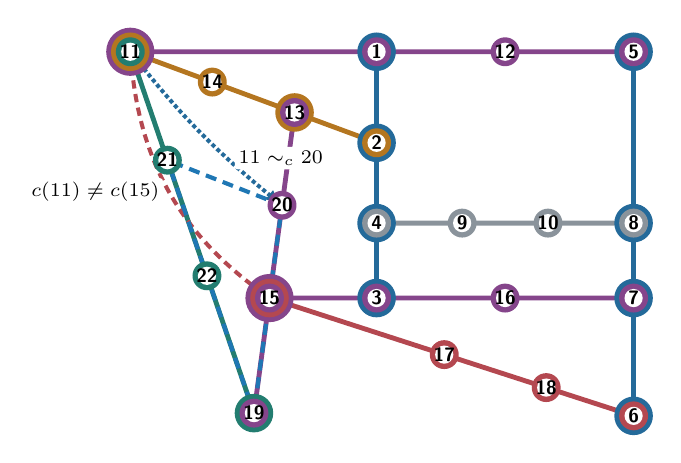
\begin{tikzpicture}[x=1cm,y=1cm,scale=0.68]
  \coordinate (v1)  at (-0.60, 3.30);
  \coordinate (v2)  at (-0.60, 1.60);
  \coordinate (v4)  at (-0.60, 0.10);
  \coordinate (v3)  at (-0.60,-1.30);
  \coordinate (v5)  at ( 4.20, 3.30);
  \coordinate (v8)  at ( 4.20, 0.10);
  \coordinate (v7)  at ( 4.20,-1.30);
  \coordinate (v6)  at ( 4.20,-3.50);
  \coordinate (v9)  at ($(v4)!.333!(v8)$);
  \coordinate (v10) at ($(v4)!.667!(v8)$);
  \coordinate (v11) at (-5.20, 3.30);
  \coordinate (v12) at ($(v1)!.50!(v5)$);
  \coordinate (v14) at ($(v11)!.333!(v2)$);
  \coordinate (v13) at ($(v11)!.667!(v2)$);
  \coordinate (v15) at (-2.60,-1.30);
  \coordinate (v16) at ($(v3)!.50!(v7)$);
  \coordinate (v17) at ($(v15)!.48!(v6)$);
  \coordinate (v18) at ($(v15)!.76!(v6)$);
  \coordinate (v20) at ($(v13)!.50!(v15)$);
  \coordinate (v19) at ($(v13)!1.62!(v15)$);
  \coordinate (v21) at ($(v11)!.30!(v19)$);
  \coordinate (v22) at ($(v11)!.62!(v19)$);

  \draw[YOtrace,YOctx1]  (v1)--(v2)--(v4)--(v3);
  \draw[YOtrace,YOctx2]  (v5)--(v8)--(v7)--(v6);
  \draw[YOtrace,YOctx4]  (v4)--(v9)--(v10)--(v8);
  \draw[YOtrace,YOctx8]  (v11)--(v1)--(v12)--(v5);
  \draw[YOtrace,YOctx9]  (v11)--(v14)--(v13)--(v2);
  \draw[YOtrace,YOctx11] (v15)--(v3)--(v16)--(v7);
  \draw[YOtrace,YOctx12] (v15)--(v17)--(v18)--(v6);
  \draw[YOtrace,YOctx5]  (v11)--(v21)--(v22)--(v19);
  \draw[YOtrace,YOctx16] (v13)--(v20)--(v15)--(v19);

  \draw[CSexcl]  (v11) to[bend right=24] node[CSnote,pos=.50,anchor=east,xshift=-2pt] {$c(11)\neq c(15)$} (v15);
  \draw[CSident] (v11) to[bend right=6]  node[CSnote,pos=.68,anchor=west,xshift=2pt] {$11\sim_c 20$} (v20);
  \draw[CSmarkedA] (v21)--(v22)--(v19)--(v20)--cycle;

  \YOvertex{1}{1/.36,8/.27}
  \YOvertex{2}{1/.36,9/.27}
  \YOvertex{3}{1/.36,11/.27}
  \YOvertex{4}{1/.36,4/.27}
  \YOvertex{5}{2/.36,8/.27}
  \YOvertex{6}{2/.36,12/.27}
  \YOvertex{7}{2/.36,11/.27}
  \YOvertex{8}{2/.36,4/.27}
  \YOvertex{9}{4/.27}
  \YOvertex{10}{4/.27}
  \YOvertex{11}{8/.45,9/.36,5/.27}
  \YOvertex{12}{8/.27}
  \YOvertex{13}{9/.36,16/.27}
  \YOvertex{14}{9/.27}
  \YOvertex{15}{11/.45,12/.36,16/.27}
  \YOvertex{16}{11/.27}
  \YOvertex{17}{12/.27}
  \YOvertex{18}{12/.27}
  \YOvertex{19}{5/.36,16/.27}
  \YOvertex{20}{16/.27}
  \YOvertex{21}{5/.27}
  \YOvertex{22}{5/.27}
\end{tikzpicture}
\caption{The strictly linear $22$-ray, $9$-context hypergraph $L_{22,9}^{(4)}$ in $\R^4$ [Eqs.~\eqref{eq:L22-contexts}--\eqref{eq:L22-vectors}], with all $9$ four-element contexts drawn as straight lines. Shown are the universally rainbow pair $c(11)\neq c(15)$, the monochromatic pair $11\sim_c 20$, and the complete rainbow quadruple $\{19,20,21,22\}$ (blue dashed polygon).}\label{fig:L22-4d}
\end{figure}

\subsection{Four-Parameter Spectral Equalities and Maximal Preparations}\label{sec:weighted-four-dimensional}

All four complete rainbow quadruples in Eq.~\eqref{eq:L22-complete4} arise by exchanging the chromatic twins $11$ and $20$ in an actual context: the first three replace $11$ by $20$ in $C_8,C_4,C_5$, respectively, and the last replaces $20$ by $11$ in $C_9$. If $C$ is that context and $t=\kappa(11)=\kappa(20)$, their weighted operators are therefore
\begin{equation}\label{eq:weighted-L22-perturbation}
O_U(\mathbf c;\kappa)=A_C(\mathbf c;\kappa)
\ \pm c_t(P_{20}-P_{11}),
\end{equation}
where the plus sign applies to the first three. This constructs the operator from an actual spectral sum followed by a rank-at-most-two Hermitian correction.

For an explicit four-parameter equality, order the first target as $U=(20,19,21,22)$ and label its colors $(0,1,2,3)$. The vector $\hat r_{19}$ is orthogonal to the other three target rays, so it is an eigenvector with eigenvalue $c_1$. The squared overlaps needed on its orthogonal complement are
\begin{equation}\label{eq:weighted-L22-overlaps}
\begin{aligned}
|\ip{\hat r_{20}}{\hat r_{11}}|^2&=\tfrac{41}{42},&
|\ip{\hat r_{20}}{\hat r_{19}}|^2&=0,\\
|\ip{\hat r_{20}}{\hat r_{21}}|^2&=\tfrac{41}{2030},&
|\ip{\hat r_{20}}{\hat r_{22}}|^2&=\tfrac{11}{3045}.
\end{aligned}
\end{equation}
The characteristic equality factors as
\begin{equation}\label{eq:weighted-L22-polynomial}
\begin{aligned}
0&=(\lambda-c_1)\bigl(\lambda^3-T\lambda^2+B\lambda-K\bigr),\\
T&=c_0+c_2+c_3,\\
B&=\tfrac{1989}{2030}c_0c_2+\tfrac{3034}{3045}c_0c_3+c_2c_3,\\
K&=\tfrac{41}{42}c_0c_2c_3.
\end{aligned}
\end{equation}
Thus the exact maximal expectation is
\begin{equation}\label{eq:weighted-L22-max}
\boxed{\begin{aligned}
\max_\rho\bigl[&c_0p_\rho(20)+c_1p_\rho(19)\\
&+c_2p_\rho(21)+c_3p_\rho(22)\bigr]
=\max\{c_1,F(T,B,K)\}.
\end{aligned}}
\end{equation}
The cubic formula gives the other three eigenvalues; Eq.~\eqref{eq:weighted-spectral-resolution} gives the full eigenspaces, including any degeneracy with $c_1$. The other quadruples follow from Eq.~\eqref{eq:weighted-L22-perturbation} or directly from the general principal-minor equality.

For unit color values, every context operator is $I_4$, so all four target operators have the same spectrum,
\begin{equation}\label{eq:weighted-L22-unit-spectrum}
\operatorname{spec}O_U(\mathbf1)
=\{1-1/\sqrt{42},\ 1,\ 1,\ 1+1/\sqrt{42}\}.
\end{equation}
Their maximal expectation is exactly $1+1/\sqrt{42}$, compared with the chromatic state-sum value one. For an explicit maximizing preparation for the first three targets, put $u=\hat r_{20}$, $v=\hat r_{11}$, $\alpha=\ip{v}{u}$, and $\varepsilon=1/\sqrt{42}$. A vector proportional to
\[
u-\frac{\alpha}{1+\varepsilon}v
\]
is an eigenvector of $P_{20}-P_{11}$ with eigenvalue $\varepsilon$; normalize it to obtain the maximizing pure state. For the fourth target, exchange $u$ and $v$. The double eigenvalue one has eigenspace $\operatorname{span}\{u,v\}^{\perp}$.

Finally, a common-apex lift sends a three-dimensional target operator to $O_X\oplus0$, adding a zero eigenvalue. If the apex is included, its color-weighted projection changes this to $O_X\oplus c_{\kappa(\mathrm{apex})}$. Hence the lifted maxima are $\max\{\lambda_{\max}(O_X),0\}$ and $\max\{\lambda_{\max}(O_X),c_{\kappa(\mathrm{apex})}\}$, respectively. The rainbow pairs of $L_{18,7}^{(4)}$ and $L_{22,9}^{(4)}$ have the two eigenvalues in Eq.~\eqref{eq:weighted-two-ray-spectrum} together with two zeros. These constructions cover the four-dimensional census using at most four independent real color parameters.

\subsection{Full Classical Bounds in Four Dimensions}\label{sec:classical-4d}

In $L_{22,9}^{(4)}$, the full two-valued state family satisfies the one-way implication $s(11)\le s(20)$. Indeed, $s(11)=1$ sets $s(13)=s(19)=0$, the $\{11,15\}$ TIFS gives $s(15)=0$, and $C_9$ then forces $s(20)=1$. The reverse implication fails on $66$ of the $158$ states. Thus the first three quadruples of Eq.~\eqref{eq:L22-complete4} have totals $1+s(20)-s(11)\in\{1,2\}$, while the last has total $1+s(11)-s(20)\in\{0,1\}$. Their common quantum spectrum in Eq.~\eqref{eq:weighted-L22-unit-spectrum} violates the lower classical bound for the first three and the upper bound for the last.

More generally, in the color order $(20,19,21,22)$ of Section~\ref{sec:weighted-four-dimensional}, the exact classical four-parameter endpoints are the minimum and maximum of
\begin{equation}\label{eq:classical-L22-envelope}
\{c_0,c_1,c_2,c_3,c_0+c_2,c_0+c_3\}.
\end{equation}
These are the bounds to compare with the four quantum roots in Eq.~\eqref{eq:weighted-L22-polynomial}. On the extendable states, only the four single-color expressions remain. The twin difference $s(11)-s(20)$ has full classical interval $[-1,0]$, whereas $P_{11}-P_{20}$ has extrema $\pm1/\sqrt{42}$.

The pair $\{11,15\}$ is already exclusive on all $68$ states of $L_{18,7}^{(4)}$, so its quantum maximum $1+1/\sqrt{42}$ exceeds the full classical bound one. The common-apex lifts preserve the corresponding base comparisons, with the additional classical possibility of selecting only the apex. Consequently the bug-tip separation persists in $B_{14,7}^{(4)}$, whereas the pair $\{14,18\}$ in $D_{17,9}^{(4)}$ still separates only the extendable-state bound. The full inventories use the separate faithful coordinates for $L_{18,7}^{(4)}$ and $L_{22,9}^{(4)}$, including their different rays $13$ and $14$.



A direct preparation already violates the full-state classical inequality $p(11)-p(20)\le0$: take $\psi=\hat r_{11}=(0,0,1,-1)^{\mathsf T}/\sqrt2$. The probabilities are
\begin{equation}\label{eq:L22-order-explicit-witness}
p_\psi(11)=1,\qquad p_\psi(20)=\frac{41}{42},
\end{equation}
giving the positive difference $1/42$. Optimizing the preparation increases this difference to $1/\sqrt{42}$, as follows from the spectrum of $P_{11}-P_{20}$.

% ==================================================================
\section{Classical--Quantum Comparison Across All Configurations}\label{sec:classical-census}
% ==================================================================

The comparison covers every configuration in Table~\ref{tab:master-chromatic-relations}. The accompanying Python inventory explicitly specifies the FOR used for each graph and reconstructs every listed context. Complete state enumeration is followed by projection to the relevant color coefficient vectors, so the classical bounds remain exact functions of arbitrary real color values. Table~\ref{tab:classical-quantum-representatives} illustrates one target per configuration at unit values; the complete machine-readable comparison contains every target expression described below.

\begin{table*}[t]
\caption{Representative unit-color comparisons for all $19$ configurations. Classical entries are sharp expectation intervals over convex mixtures of all two-valued states ($\Sc$) or only extendable states ($\Sc_{\mathrm{ext}}$). Quantum entries are the extremal eigenvalues for the specified FOR, rounded to six decimal places. The last column identifies separation from the full classical interval, not merely from the extendable-state interval. The selected row for a configuration need not maximize its separation. The accompanying tables retain every expression.}\label{tab:classical-quantum-representatives}
\footnotesize\renewcommand{\arraystretch}{1.35}\setlength{\tabcolsep}{5pt}
\begin{ruledtabular}
\begin{tabular}{llcccc}
Configuration & Target & Classical on $\Sc$ & Classical on $\Sc_{\mathrm{ext}}$ & Quantum interval & Separation\\\hline
$M_{15,8}$ & $\{1,6,11\}$ & $[0,2]$ & $[0,2]$ & $[0.172673,2.000000]$ & none\\
$\mathsf H_{20}$ & $\{a_1,a_2\}$ & $[0,2]$ & $[0,2]$ & $[0.000000,1.553775]$ & none\\
$B_{13,7}$ & $\{10,11\}$ & $[0,1]$ & $[0,1]$ & $[0.000000,1.333333]$ & upper\\
$D_{16,9}$ & $\{14,18\}$ & $[0,2]$ & $[0,1]$ & $[0.000000,1.088889]$ & none\\
$I_{16,9}$ & $\{10,11\}$ & $[0,1]$ & $[0,1]$ & $[0.000000,1.272166]$ & upper\\
$H_{17,10}$ & $\{10,11\}$ & $[0,1]$ & $[0,1]$ & $[0.000000,1.333333]$ & upper\\
$T_{19,11}$ & $\{9,26\}$ & $[0,1]$ & $[0,1]$ & $[0.000000,1.252415]$ & upper\\
$H_{20,12}$ & $\{15,18,20\}$ & $[1,3]$ & $[1,1]$ & $[0.729610,1.234838]$ & lower\\
$H_{21,13}$ & $\{10,11,13\}$ & $[0,1]$ & $[1,1]$ & $[0.333333,1.333333]$ & upper\\
$G_{27,16}$ & $\{3,14,18\}$ & $[1,1]$ & $[1,1]$ & $[0.794691,1.205309]$ & both\\
$G_{41,25}$ & $\{3,27,28\}$ & $[1,1]$ & $[1,1]$ & $[0.798527,1.210746]$ & both\\
$G_{41,26}$ & $\{3,27,28\}$ & $[1,1]$ & $[1,1]$ & $[0.682383,1.359339]$ & both\\
$H_{53,34}$ & $\{a,b,u\}$ & $[1,1]$ & $[1,1]$ & $[0.570956,1.516521]$ & both\\
$R_{21,12}$ & $\{1,17,18\}$ & $[0,3]$ & $[0,3]$ & $[0.500000,1.762348]$ & none\\
$R_{25,15}$ & $\{1,17,18\}$ & $[0,3]$ & $[0,3]$ & $[0.500000,1.762348]$ & none\\
$B_{14,7}^{(4)}$ & $\{10,11\}$ & $[0,1]$ & $[0,1]$ & $[0.000000,1.333333]$ & upper\\
$D_{17,9}^{(4)}$ & $\{14,18\}$ & $[0,2]$ & $[0,1]$ & $[0.000000,1.088889]$ & none\\
$L_{18,7}^{(4)}$ & $\{11,15\}$ & $[0,1]$ & $[0,1]$ & $[0.000000,1.154303]$ & upper\\
$L_{22,9}^{(4)}$ & $\{19,20,21,22\}$ & $[1,2]$ & $[1,1]$ & $[0.845697,1.154303]$ & lower\\

\end{tabular}
\end{ruledtabular}
\end{table*}

The exhaustive target inventory contains $2{,}289$ single-set sums, $931$ signed size-two or size-three paired differences, and $50$ twin differences: $3{,}270$ expressions in total. Single-set sums include actual contexts as consistency checks, all non-context complete rainbow sets, independent universally rainbow subsets, nontrivial twin subsets, and both components of every counted paired relation. Paired relations use the census convention excluding pairs of two already complete independent admissibility contexts. Restricting every normalized strong coloring to each expression, and identifying restrictions related by a palette permutation, gives $10{,}873$ color patterns. This covers every coloring and every real assignment to its used colors; it does not enumerate arbitrary unlisted subsets of vertices.

For every pattern, the saved integer vectors define both classical envelopes in Eq.~\eqref{eq:classical-envelopes}. Testing all classical facets and both signs of the affine equalities gives the comparison counts in Table~\ref{tab:classical-quantum-coverage}. Unit values already separate $663$ expressions from the full state family; allowing general real color values increases this number to $1{,}445$. These are overlapping target expressions, not $1{,}445$ independent contextuality proofs. A zero entry rules out separation within the listed color-weighted expression family and chosen FOR to the reported numerical precision; it does not establish a classical model for other observables or other FORs.

\begin{table*}[t]
\caption{Coverage and separation counts for the full comparison. The triple $X/D/T$ counts single-set sums, multiset-pair differences, and twin differences, respectively. $U_{\Sc}$ counts expressions separated from $\conv\Sc$ at unit color values. $W_{\Sc}$ and $W_{\mathrm{ext}}$ count expressions admitting a separating real color assignment for at least one restricted color pattern, using the complete facet/equality test on the indicated state family. Both spectral endpoints are included. Actual contexts are part of $X$ but never contribute a separation. Counts depend on the stated FORs.}\label{tab:classical-quantum-coverage}
\footnotesize\renewcommand{\arraystretch}{1.35}\setlength{\tabcolsep}{10pt}
\begin{ruledtabular}
\begin{tabular}{lccccc}
Configuration & $|\Sc_{\mathrm{ext}}|/|\Sc|$ & $X/D/T$ & $U_{\Sc}$ & $W_{\Sc}$ & $W_{\mathrm{ext}}$\\\hline
$M_{15,8}$ & $24/24$ & $16/4/0$ & $0$ & $0$ & $0$\\
$\mathsf H_{20}$ & $26/26$ & $54/21/0$ & $0$ & $0$ & $0$\\
$B_{13,7}$ & $12/14$ & $10/1/0$ & $1$ & $1$ & $1$\\
$D_{16,9}$ & $14/21$ & $10/0/0$ & $0$ & $0$ & $1$\\
$I_{16,9}$ & $12/22$ & $37/5/2$ & $13$ & $13$ & $26$\\
$H_{17,10}$ & $10/18$ & $44/5/2$ & $13$ & $13$ & $32$\\
$T_{19,11}$ & $14/25$ & $31/3/2$ & $2$ & $2$ & $17$\\
$H_{20,12}$ & $10/25$ & $110/32/4$ & $21$ & $38$ & $117$\\
$H_{21,13}$ & $6/21$ & $199/36/21$ & $30$ & $45$ & $207$\\
$G_{27,16}$ & $54/82$ & $74/14/2$ & $42$ & $46$ & $50$\\
$G_{41,25}$ & $216/396$ & $173/39/6$ & $120$ & $139$ & $146$\\
$G_{41,26}$ & $63/107$ & $571/318/6$ & $186$ & $484$ & $620$\\
$H_{53,34}$ & $128/224$ & $841/428/4$ & $227$ & $656$ & $844$\\
$R_{21,12}$ & $48/54$ & $33/12/0$ & $0$ & $0$ & $0$\\
$R_{25,15}$ & $48/81$ & $36/12/0$ & $0$ & $0$ & $0$\\
$B_{14,7}^{(4)}$ & $13/15$ & $10/1/0$ & $1$ & $1$ & $1$\\
$D_{17,9}^{(4)}$ & $15/22$ & $10/0/0$ & $0$ & $0$ & $1$\\
$L_{18,7}^{(4)}$ & $68/68$ & $8/0/0$ & $1$ & $1$ & $1$\\
$L_{22,9}^{(4)}$ & $92/158$ & $22/0/1$ & $6$ & $6$ & $13$\\

\end{tabular}
\end{ruledtabular}
\end{table*}

\subsection{Enumeration and Numerical Verification}

The supplied Python translation of Tkadlec's program~\cite{tkadlec-2states-2017} agrees, state by state, with the new block-recursion implementation and an independent variable-first propagation solver for all $19$ configurations. A further $240$ small complete-block/proper-subblock problems agree with exhaustive binary enumeration. No state-generation discrepancy was found for the covered vertex sets. The legacy Pascal executable could not be launched on the verification host, so no Pascal execution or compilation is claimed. The new module ports the state-generation algorithm, not the original potentially incomplete element-separation and order-determination heuristics; those heuristics are unnecessary for Eq.~\eqref{eq:classical-envelopes}. The original source and supplied translation are preserved with the calculation.

The legacy programs assume that every declared atom occurs in a listed block or subblock. An unused declared atom is silently fixed to zero; the new implementation instead enumerates it freely. This difference does not affect the present hypergraphs, for which $V=\bigcup E$. The new program also removes the fixed array limits and writes results separately rather than overwriting its input. Every configuration has a dense Pascal-format input/state file together with an explicit map back to the manuscript's ray labels.

All state, extendability, and normalized-coloring counts agree with the manuscript census. The only relation-count correction is the octagon's $20$ size-three affine pairs, with an explicit certificate in Eq.~\eqref{eq:octagon-size3-correction}. For every chosen FOR, all contexts resolve the identity, all intended orthogonal pairs are verified, all nonedges have nonzero inner product, and all rays are distinct. The separate coordinates for deleted-context restrictions, roof cascades, and four-dimensional examples are retained; a nonfaithful restriction of a larger FOR is not substituted for them.

There are $218$ distinct classical coefficient polytopes. Their integer facet planes are reconstructed exactly and checked against every state coefficient vector; an independent enumeration of all possible supporting hyperplanes reproduces every facet list. Quantum eigenvalues for $20{,}527$ distinct signed operators are independently recomputed at $80$ decimal digits, verifying all $100{,}495$ facet/equality comparisons and every unit expression. The largest discrepancy from the working double-precision extrema is below $3.1\times10^{-15}$. Reported strict separations exceed $10^{-9}$; the smallest positive gap in the scan is greater than $7.2\times10^{-4}$. Maximizing vectors and their residuals are saved with the witnesses. These are numerical spectral comparisons with exact classical bounds, not a global optimization of gap magnitude over coefficients or FORs.

The files \texttt{unit-comparison.csv} and \texttt{weighted-witnesses.csv} give all unit expressions and separating parameter choices. Each configuration's JSON record contains its complete states and colorings, every distinct restricted color pattern, both exact finite classical envelopes, affine equalities, facet inequalities, and spectral comparisons. The evaluator accepts arbitrary real color values and can construct the exact symbolic operator and characteristic polynomial from the algebraic ray formulas. Thus the calculation is reproducible without the missing certificate referenced by the older verifier.

% ==================================================================
\section{Master Census and Conclusion}\label{sec:conclusion}
% ==================================================================

Table~\ref{tab:master-chromatic-relations} summarizes the invariants and admissibility relations of all $19$ configurations, including $H_{53,34}$. Its two independent chromatic admissible triples, $\{a,b,u\}$ and $\{a',b',u\}$, also satisfy the stronger two-valued state admissibility condition. The paired columns omit equivalences between two already complete admissibility contexts, as specified in Definition~\ref{def:chromatic-relations}.



The central phenomenon is enforced exclusivity and completeness on a single independent set, stratified into a three-tier hierarchy by the underlying state family:
\begin{enumerate}
\item \emph{Chromatic admissible contexts on $\Sc_{\mathrm{ext}}(H)$:} Rainbow in every strong $d$-coloring, or equivalently normalized ($\sum_{u\in U}s(u)=1$) on every extendable color-class state. In the Yu--Oh family, pairwise-nonorthogonal chromatic admissibility triples first appear at $12$ contexts ($H_{20,12}$, $2$ triples) and reach $21$ triples in $H_{21,13}$ (Theorem~\ref{thm:H21-complete}), including the coplanar triple $U_{\mathrm{cop}}=\{3,6,9\}$ and the $60^\circ$ basis $U_{\mathrm{core}}=\{1,4,7\}$.
\item \emph{Two-valued admissibility contexts on $\Sc(H)$:} Normalized ($\sum_{u\in U}s(u)=1$) on \emph{every} admissible two-valued state $s\in\Sc(H)$. Even though no linear combination of context equations can force a nonorthogonal $d$-tuple to sum to $1$ on $\mathcal A(H)$ (Proposition~\ref{prop:no-operator-complete}), $\{0,1\}$-integrality on Specker bugs across two-context roofs enforces biconditional two-valued twins $s(x)=s(x')$ (Lemma~\ref{lem:roof-twin}), causing $\operatorname{aff}\Sc(H)\subsetneq\mathcal A(H)$ and yielding the pairwise-nonorthogonal two-valued state admissibility context $U_{\mathrm{TVS}}=\{3,27,28\}$ in $G_{41,25}$ and $G_{41,26}$ (Theorem~\ref{thm:tvs-admissibility}). Proposition~\ref{prop:yo-binary-filters} gives additional binary state restrictions for $H_{20,12}$ and $H_{21,13}$; faithful geometric realizations of simultaneous gadget attachments are not claimed. The $53$-ray construction of Section~\ref{sec:two-valued} gives two further independent two-valued state admissibility contexts and an explicit Born-state total $8/9$, with a full hypergraph drawing and exact coordinate certificate.
\item \emph{Operator and affine rigidity on $\Wc(H)$ and $\mathcal A(H)$:} No nonorthogonal $d$-tuple can resolve the identity $\sum_{u\in U}P_u=I_d$ or be normalized on $\mathcal A(H)$. Meanwhile, balanced context certificates yield paired affine pseudocontexts ($M_{15,8}$ and $\Htwenty$), which imply color-multiset equivalence on $\Sc_{\mathrm{ext}}(H)$ without requiring single-set completeness.
\end{enumerate}

The color-weighted construction turns these assignment-level relations into explicit probability witnesses with exact classical parameter envelopes. In $H_{53,34}$, the classical normalization total one has quantum range approximately $[0.570956,1.516521]$. The additional facet $p(u)-p(y_5)+p(y_9)\le1$ has quantum maximum approximately $1.545526$, revealing a separation absent from the unweighted sum of the same three projectors. Proposition~\ref{prop:H53-weighted-facet} supplies both a binary implication proof and an optimal quantum preparation.

Classical completeness also yields lower-bound witnesses: the two $H_{20,12}$ triples have full classical total at least one but quantum minimum approximately $0.729610$. The core and coplanar triples of $H_{21,13}$ remain inside their full projected classical polytopes, whereas its hub triple violates the upper bound one with total $4/3$. Exact equality and order witnesses complement these sums: $G_{41,26}$ permits a quantum difference $p(11)-p(18)=1/3$ against the classical equality zero, and $L_{22,9}^{(4)}$ permits $p(11)-p(20)=1/\sqrt{42}$ against the classical upper bound zero.

These examples exclude convex mixtures of all admissible two-valued states. Comparisons using only extendable states are identified separately in Tables~\ref{tab:classical-quantum-representatives} and~\ref{tab:classical-quantum-coverage}. The full comparison covers $19$ configurations with fixed faithful representations; the violating preparations depend on the chosen FOR and coefficient values. All these probability witnesses are state-dependent: the maximally mixed quantum assignment is already a classical mixture of color-class states, as shown in Remark~\ref{rem:state-dependent-witnesses}.

\begin{acknowledgments}
This research was funded in part by the Austrian Science Fund (FWF), Grant DOI \href{https://doi.org/10.55776/PIN5424624}{10.55776/PIN5424624}.
\end{acknowledgments}

\def\doibase{https://doi.org/}
\bibliography{svozil}

\end{document}
